\documentclass[soumission]{jsfds}
\usepackage[utf8]{inputenc}

%\DeclareUnicodeCharacter{00FC}{\u}
%\DeclareUnicodeCharacter{00E9}{\e}
%\DeclareUnicodeCharacter{00E0}{\a}

\usepackage[T1]{fontenc}

\usepackage{hyperref} 
\usepackage{amsmath,amsthm} 
\usepackage[english]{babel}
\usepackage{graphicx}
\usepackage{natbib} 
\usepackage{jsfds}
\usepackage{caption}
\usepackage{breakcites}
\usepackage{hyperref}
\usepackage{todonotes}
\usepackage{bm}
\usepackage{stmaryrd} 
\usepackage{array} 

\usepackage{tikz}
\usepackage{color}
\usepackage{multirow}
\usepackage{ulem} % pour barrer de texte

\usepackage[toc,page]{appendix}
\usepackage{tocloft}


\usetikzlibrary{calc,shapes,backgrounds,arrows,automata,shadows,positioning}

\newcommand{\prior}{\textit{prior }}
\newcommand{\posterior}{\textit{posterior }}

\newcommand{\EqRef}[1] {Equation (\ref{#1})}
  
\startlocaldefs
% Commandes auteurs spécifiques, par exemple :
\newcommand{\EP}[1]{\textcolor{blue}{(eric): #1}}
\newcommand{\R}{\mathbb{R}}
\newcommand{\E}{\mbox{\tiny \`eme}}
\def\1{1\kern-.20em {\rm l}}
\endlocaldefs

\colorlet{darkyellow}{yellow!50!black}

\startlocaldefs
\newcommand{\MCC}[1]{\textcolor{darkyellow}{(mathieu): #1}}
\endlocaldefs

\edef\hc{\string: }

\setmainlanguagefrench
\firstpage{1} 
\newcommand{\PB}[1]{\textcolor{green}{PB: #1}}

\begin{document}

\begin{frontmatter}

  % infos fournies par l'éditeur, laisser vide
  % \volume{}
  % \numero{}
  % \anneepublication{}
  % \doi{}
  %\arxiv{math.PR/00000000} 

  \titre{Bayesian calibration of a numerical code for prediction}
  \titrealter{Theory of code calibration and application to the prediction of a photovoltaic power plant electricity production}

\begin{aug}
    \auteur{
      \prenom{Mathieu} 
      \nom{Carmassi}
      \thanksref{t1,t2,t3}
      \contact[label=e1]{mathieu.carmassi@edf.fr}
      \contact[label=e1Bis]{mathieu.carmassi@agroparistech.fr}
      	}
    \and
    \auteur{
      \prenom{Pierre} 
      \nom{Barbillon}
      \thanksref{t2}
      \contact[label=e2]{pierre.barbillon@agroparistech.fr}
    	}
    \and
    \auteur{
      \prenom{Merlin} 
      \nom{Keller}
      \thanksref{t3}
      \contact[label=e4]{merlin.keller@edf.fr}
	    }
	\and
    \auteur{
      \prenom{Eric} 
      \nom{Parent}
      \thanksref{t2}
      \contact[label=e5]{eric.parent@agroparistech.fr}
  		}
    \and
    \auteur{
      \prenom{Matthieu} 
      \nom{Chiodetti}
      \thanksref{t1}
      \contact[label=e3]{matthieu.chiodetti@edf.fr}
    	}

     \affiliation[t1]{EDF R\&D, TREE department, Moret-sur-Loing 
     }
     \affiliation[t2]{UMR MIA-Paris, AgroParisTech, INRA, Paris 
%     \printcontact{e2}, \printcontact{e5} and \printcontact{e1Bis} 
     }
     \affiliation[t3]{EDF R\&D, PRISME department, Chatou 
%     \printcontact{e4} and \printcontact{e1}%
     }
     \enteteauteurs{Carmassi, Barbillon, Chiodetti, Keller and Parent}
  \end{aug}

\begin{abstract}
Les difficultés de mise en oeuvre d'expériences de terrain ou de laboratoire, ainsi que les coûts associés, conduisent les sociétés 
industrielles à se tourner vers des codes numériques de calcul. Ces codes, censés être représentatifs des phénomènes physiques en jeu, 
entraînent néanmoins tout un cortège de problèmes. Le premier de ces problèmes provient de la volonté de prédire la réalité à partir d'un 
modèle informatique. En effet, le code doit être représentatif du phénomène et, par conséquent, être capable de simuler des données proches de  
la réalité. Or, malgré le constant développement du réalisme de ces codes, des erreurs de prédiction subsistent. Elles sont de deux natures différentes. La
première provient de la différence entre le phénomène physique et les valeurs relevées expérimentalement. La deuxième concerne l'écart entre le code développé et le phénomène physique. Pour diminuer cet écart, souvent qualifié de biais ou d'erreur de modèle, les développeurs complexifient en général les codes, les rendant très chronophages dans certains cas. De plus, le code dépend de paramètres à fixer par l'utilisateur qui doivent être choisis pour correspondre au mieux aux données de terrain. L'estimation de ces paramètres propres au code s'appelle le calage.
Ce papier propose une revue des méthodes de calage bayésien et s'appuie sur un cas d'application qui permet de discuter les divers choix méthodologiques et d'illustrer leurs divergences. Cet exemple s'appuie sur un code de calcul servant à prédire la puissance d'une centrale photovoltaïque. 


\end{abstract}
  

\begin{altabstract}
Field experiments are often difficult and expensive to make. To bypass these issues, industrial companies have developed computational codes. These codes intend to be representative of the physical system, but come with a certain amount of problems. The code intends to be as close as possible to the physical system. It turns out that, despite continuous code development, the difference between the code outputs and experiments can remain significant. Two kinds of uncertainties are observed. The first one comes from the difference between the physical phenomenon and the values recorded experimentally. The second concerns the gap between the code and the physical system. To reduce this difference, often named model bias, discrepancy, or model error, computer codes are generally complexified in order to make them more realistic. These improvements lead to time consuming codes. Moreover, a code often depends on parameters to be set by the user to make the code as close as possible to field data. This estimation task is called calibration. This paper proposes a review of Bayesian calibration methods and is based on an application case which makes it possible to discuss the various methodological choices and to illustrate their divergences. This example is based on a code used to predict the power of a photovoltaic plant. 

\end{altabstract}

  \begin{motscles}
    \mot{Centrale photovoltaïque}%
    \mot{Calage bayésien}%
    \mot{Quantification d'incertitudes}
    \mot{Code numérique}
  \end{motscles}

  \begin{motsclesalter}
    \mot{Photovoltaic power plant}
    \mot{Bayesian calibration}
    \mot{Uncertainty quantification}
    \mot{Numerical code}
  \end{motsclesalter}
  
  \begin{AMSclass}
    \kwd{35L05}
    \kwd{35L70}
  \end{AMSclass}
 
\end{frontmatter}


\section{Introduction}

%\paragraph{Pourquoi, contexte ?}

Numerical experiments have become increasingly popular in many (if not all) industrial fields. Indeed, setting up field experiments can represent a huge investment for a company. Numerical simulations are generally considered as a substitute to bypass physical or field experiments \citep{santner2013,fang2005}. However, the complexity of computer codes, used in such simulations, increases with the capacity of computer processors, and sometimes at a much higher rate. The consequence is straightforward\hc some codes have become greedy in computational time \citep{sacks1989}. Moreover, a gap between computer code outputs and field measures of the physical process, sought to simulate, is routinely observed. 
Checking the accuracy of the code by confronting it with field experiments is called validation \citep{bayarri2007}. This task is difficult since it is based on a few unavoidable field data and a computational code, often long to run. 
All along this paper, we will use the word ``code'' as a proxy for numerical code, sometimes also called numerical model, simulator or computational code and field experiment for real world experiment.
\newline

%\paragraph{Types d'entrées -> calibration}

The code generally depends on two kinds of inputs\hc variables and parameters.
The variables are input variables (observable and often controllable) which are set during a field experiment and can encompass environmental variables that can be measured.
The parameters are generally interpreted as physical constants defining the mathematical model of the system of interest, but can also contain so-called tuning parameters, which have no physical interpretation. They have to be set by the user to run the code and chosen carefully to make the code mimic the real physical phenomenon. 
The code can be mathematically represented by a function $f_c$. Let us note, in what follows, $\boldsymbol{\theta}\in\mathcal{Q}\subset\mathbb{R}^p$ to represent the parameter vector and $\mathbf{x}\in\mathcal{H}\subset \mathbb{R}^d$ for the variable vector. The space $\mathcal{Q}$ is called the input parameter space and $\mathcal{H}$ the input variable space.
The physical phenomenon is denoted by $\zeta$ and only depends on variables in vector $\boldsymbol{x}\in\mathcal{H}$, the parameter vector $\boldsymbol{\theta}$ having no counterpart in field experiments. \newline

A code output is then written as $f_c(\boldsymbol{x},\boldsymbol{\theta})$ whereas $\zeta(\boldsymbol{x})$ denotes the output of the physical phenomenon for the same variable $\boldsymbol{x}$. This is of course an idealized formalization, in which we assume that the code variables $\boldsymbol{x}$ are exhaustive to describe the phenomenon of interest, in the sense that the quantity to be predicted can take a single deterministic value $\zeta(\boldsymbol{x})$ for a given $\boldsymbol{x}$. 
In this paper, the quantity of interest is assumed to be a scalar but 
extensions with high dimension outputs are
possible \citep{higdon2008}. 
Therefore, in what follows, the images of $\zeta$ and $f_c$ lie in $\mathbb{R}$.
\newline

We consider that a vector of field data ($\boldsymbol{y}_{exp}$), which are noisy measurements of $\zeta$, is observed as a realization of the statistical model\hc

\begin{equation*}
\mathcal{M}_0\ : \ \forall i \in \llbracket1,\dots,n\rrbracket \quad y_{exp_i}=\zeta(\boldsymbol{x}_i)+\epsilon_i
\end{equation*}

where $\forall i \in \llbracket1,\dots,n\rrbracket \quad \epsilon_i\overset{iid}{\sim} \mathcal{N}(0,\sigma_{err}^2)$. The corresponding values of the variables $\boldsymbol{x}_i$ are also observed.
\newline

Calibrating the code consists
in making the vector of parameters $\boldsymbol{\theta}$ consistent in some sense with these $n$ field data. In an industrial framework, uncertainty quantifications \citep{rocquigny2009quantifying} can be decomposed into a step by step procedure and calibration is identified as a key element of the so-called \textit{step B'}. As illustrated in \citet{damblin2015}, this step concerns calibration,
verification and validation (V\&V). V\&V can be further split into 3 phases  described in \citet{roache1998}, \citet{bayarri2007} and \citet{oberkampf1998}.
Calibration then aims at finding the "best" parameter vector $\boldsymbol{\theta}=\boldsymbol{\theta}^*$ such that the error term made by the
code in a statistical model is minimal. Several statistical modeling strategies have been proposed in the literature. When only measurement errors
are considered, \citet{cox2001} use a rather simple model, considering that the code does not differ from the phenomenon under study. As for
\citet{higdon2004}, \citet{kennedy2001} and \citet{bayarri2007},  they advocate some extensions, which additionally encompass a \textit{model bias} 
or a \textit{model error} term, also dubbed \textit{discrepancy} in the following. All of these models are reviewed and discussed in Section
\ref{sec:calibration}. The identifiability issues between the parameter $\boldsymbol{\theta}$ and the discrepancy were already discussed in the written discussions of \citet{kennedy2001}. \citet{tuo2015efficient} consider the calibration task as a minimization of a loss function between the code and the physical reality. 
In \citet{tuo2016theoretical}, 
%they interpret the definition of \citet{kennedy2001} for $\boldsymbol{\theta}$ (the ``best-fitting'' parameter) as being the minimizer of the reproducing kernel Hilbert space norm based on the prior distribution of the discrepancy.
they show that this loss function leads to an estimation of $\boldsymbol{\theta}$ depending on the chosen prior distribution of the discrepancy. Then,  \citet{plumlee2017} advices an orthogonality 
specification for the discrepancy i.e. the discrepancy should be orthogonal to the gradient of the computer code with respect to a loss function.
\newline


As an industrial illustrative example, we will focus, in this paper, on predicting the energy production from a photovoltaic (PV) plant \citep{martin2001}. The industrial context is to go through proposals as a manufacturer and a supplier for PV plants. The selling price announced by the industrial company has to be competitive enough to be successful in the bidding process. Of course, the building costs and the production over the plant lifetime have to be known to evaluate the profit margins. Although a best guess-estimate, the deterministic evaluation of PV production through a sophisticated computer code, does not fulfill the needs of a financial investor in  PV projects. To evaluate the financial risks of his/her investment and consequently to make his decision, the investor needs to assess the uncertainty around the expected production estimation. To do so, all the sources of uncertainties have to be identified and treated in their current form. Calibration will be useful for hunting down the uncertainties related to the modeling and quantify the range of the main potential errors made in predicting the profit ratio.\newline


%\paragraph{Plan de l'article}

This paper first presents the illustrative case study (Section \ref{PVsection}). The stakes are given with the explanation of the code and the source of the experimental data. Section \ref{sec:calibration} deals with the presentation of the many different statistical models one can find in the literature which have been developed for calibration. Then, a highlight of the different likelihoods and conditional densities needed for parameter estimation is provided. In Section \ref{sec:application}, the different statistical models are implemented and tested for the PV application case, in order to illustrate the various ways of reasoning behind calibration and point out their differences.



\section{Production estimation from a PV plant \label{PVsection}}

\subsection{Stakes}

Today, the market in electricity production has become more and more competitive. Environmental issues have brought changes in such a way that producing electricity by exploiting sun-power has become a popular and a major vector of green production. However, building a PV plant represents a lot of financial risks. Indeed, many factors must be taken into account before computing the return rate. The overall building cost is the first figure needed but can easily be estimated. Once it is evaluated, a prediction of the PV plant production will set up the return rate. To compute such a prediction, a code has been developed, implementing a mathematical model which aims at reproducing the physical system of the plant. \newline

However, there are two major sources of uncertainty linked to this method. The first one is the meteorological data which we have difficulties to predict, especially in the changing environment due to global warming. In a project framework, we will usually use the meteorological data based on the previous years with past scenarios eventually adjusted to take into account temperature increase. The second source of uncertainties comes from the modeling errors. The code may encounter difficulties to mimic the physical system. As discussed above, this can be explained by the fact that the mathematical model implemented is only a simplified representation of the physical world, which might not take into account all the existing influent variables, and also depends on uncertain physical constants, which are precisely the parameters we wish to estimate. \newline

Consequently, the error made by the output of the code straightforwardly impacts the uncertainty on the estimation of production. In this article, we will focus only on the modeling errors. Practically these errors are responsible for one half ($4\%$) of the error made on the total energy given by the plant ($8\%$).

\subsection{Source of the code}


To understand how the phenomenon has been coded, some explanation about how the PV cell works is needed. A PV cell is mainly composed of a semi-conductor material. For most technologies, this material is silicon \citep{luque2011}. The energy supply from the sun is remarkable at a quantum level. Indeed, the energy from the light spectrum will modify the energy levels of the silicon atoms until one electron appears. In a single crystal of semiconductor, two parts are visible. The ``p'' (positive) side which contains an excess of holes and the "n" side which contains an excess of electrons. A hole is an excess of a positive charge. The electron is by diffusion straightforwardly attracted to the hole, creating an electron/hole pair. The principle is to capture enough solar energy to create such an electron/hole pair. The displacement of an electron is directly  translated into electric current. The, so called, ``energy gap'', which has to be brought, corresponds to the difference between the energy of conduction band and the valence band. To create electricity, the incident solar ray on the PV cell has to have a spectrum energy higher than the energy gap. That is why, cloudy days are not favorable for PV plants production. The PV cell has a plastic film and a cover glass to protect the silicon. Otherwise, the lifetime of the cell would be too short because of its degradation. These protections act as a filter for the sun rays and some spectrum energy is lost. All in all, lots of conditions have to be met and only $20\%$ of the initial spectrum is at best transformed into electricity \citep{martin2001}. \newline


The code, hereafter considered as a ``black box'', is a solver of the main equations mimicking the electrical behavior of the PV plant. All along the article the code will represent a PV test stand with 12 panels connected together. The considered power will be the one before the inverter (multiplication of the continuous current and continuous voltage). Fortunately, for an in-depth exploration of the complete range of situations encountered in the domain of Bayesian calibration of computer codes, the ``black box'' code $f_c$ appears to be fast for the case study (one launch needs only $39\mu s$ to run). To investigate what happens when the code is time consuming, we will simply slow it down by restructuring the number of runs allowed for the computer code $f_c$.
%, as an artificial dirty but fruitful trick played to the computer code.
The code depends on some parameter vector $\boldsymbol{\theta}$ and input variables $\boldsymbol{x}$ detailed as follows (also called general inputs in \citet{plumlee2017}): $\boldsymbol{\theta}=\begin{pmatrix}
\eta \\
\mu_t \\
n_t \\
a_l \\
a_r\\
n_{inc}
\end{pmatrix}$ and $\boldsymbol{x}=\begin{pmatrix}
t\\
L\\
l\\
I_g\\
I_d \\
T_e
\end{pmatrix}$. \newline

The physical meaning of parameters is explained below \citep{duffie2013}\hc 
\begin{itemize}
\item $\eta$\hc module photo-conversion efficiency,
\item $\mu_t$\hc module temperature coefficient (the efficiency decreases when the temperature rises) in \%/°$C$,
\item $n_t$\hc reference temperature for the normal operating conditions of the module in °$C$,
\item $a_l$\hc reflection power of the ground (albedo),
\item $a_r$\hc describe the transmission of the radiation as a function of the incidence angle of solar rays, which depends on optical properties and the cleanliness,
%\item $h_{cw}$, $h_{c}$: convection coefficients
\item $n_{inc}$\hc transmission factor for normal incidence. \newline
\end{itemize}

The input variables contain all measurable data\hc 
\begin{itemize}
\item $t$\hc the UTC time since the beginning of the year in $s$,
\item $L$\hc the latitude in °,
\item $l$\hc the longitude in °,
\item $I_g$\hc global irradiation (normal incidence of the sun ray to the panel) in $W/m^2$,
\item $I_d$\hc diffuse irradiation (horizontal incidence of the sun ray to the panel) in $W/m^2$,
\item $T_{e}$\hc ambient temperature in  °$C$.\newline
\end{itemize}


Note that some temporal aspect is taken into account through the input variables. We do not consider any delay in the PV reaction to the forcing conditions. Time $t$ indicates here a snap shot corresponding to the instant when the power has to be computed. This code only focuses on a specific time and if the evolution of the power over a day is what we look for, a repetition over the specific durations has to be made. This operation has to consider the number of time steps available. For example, if $300$ configurations of $\boldsymbol{x}$ are accessible for one day, the code will have to be executed $300$ times to have the power evolution over a day. For the rest of the article, we will denote the code output referring to the i\textsuperscript{th} time step by $f_c(\boldsymbol{x}_i,\boldsymbol{\theta})$ and by $f_c(\textbf{X},\boldsymbol{\theta})$ the code outputs corresponding to the whole time frame contained in matrix $\textbf{X}$. \newline

A sensitivity analysis performed according to the screening method of Morris \citep{morris1991} has showed that only the variations of $\eta$, $\mu_t$ and $a_r$ have a significant impact on the power. This sensitivity analysis consists in evaluating with elementary displacements in a normalized input space, the responses to these displacements on the output. To testify that $\eta$, $\mu_t$ and $a_r$ have a significant impact over a whole duration but not instantaneously a PCA (Principal Component Analysis) is performed on all outputs generated for the duration and for all combinations of the design of experiments (DOE) of Morris. On the new uncorrelated basis of the space, the information is summed up by a new Morris plot. This representation allows to visualize all the information summarized over the duration on one plot. However, to  implement such a method, the input space parameter needs to be well defined. That is why the work of the experts is really important. They have to define the range of each parameter as best as they can.\newline



\subsection{Available data}

As mentioned above, the code represents a test stand of 12 panels. Data are available over 2 months and instantaneous power is collected every $10s$, which makes around $777,600$ points to process. Data are particularly treated when recording facilities are interrupted for some reasons. Figure \ref{fig:PowerExample} shows the kind of data collected from the stand over one month (on the left) and detailed for one day (on the right). Some days the production sticks to $0$. This typically happens when recording errors occur. Actually, the power saved is aberrant with too much high or 
negative power. Data cleaning allows to detect and sort these errors. On the right panel of Figure \ref{fig:PowerExample}, we can notice a typical behavior of an assembly of solar panels. When the irradiation of the sun is high, so is the production. As expected, the maximum production happens around noon when the irradiation is high.

\begin{figure}[htbp!]
\begin{center}
  \begin{tabular}{c @{} c c}
    \rotatebox{90}{ \hspace{7em} \small Power in $W$}
    & 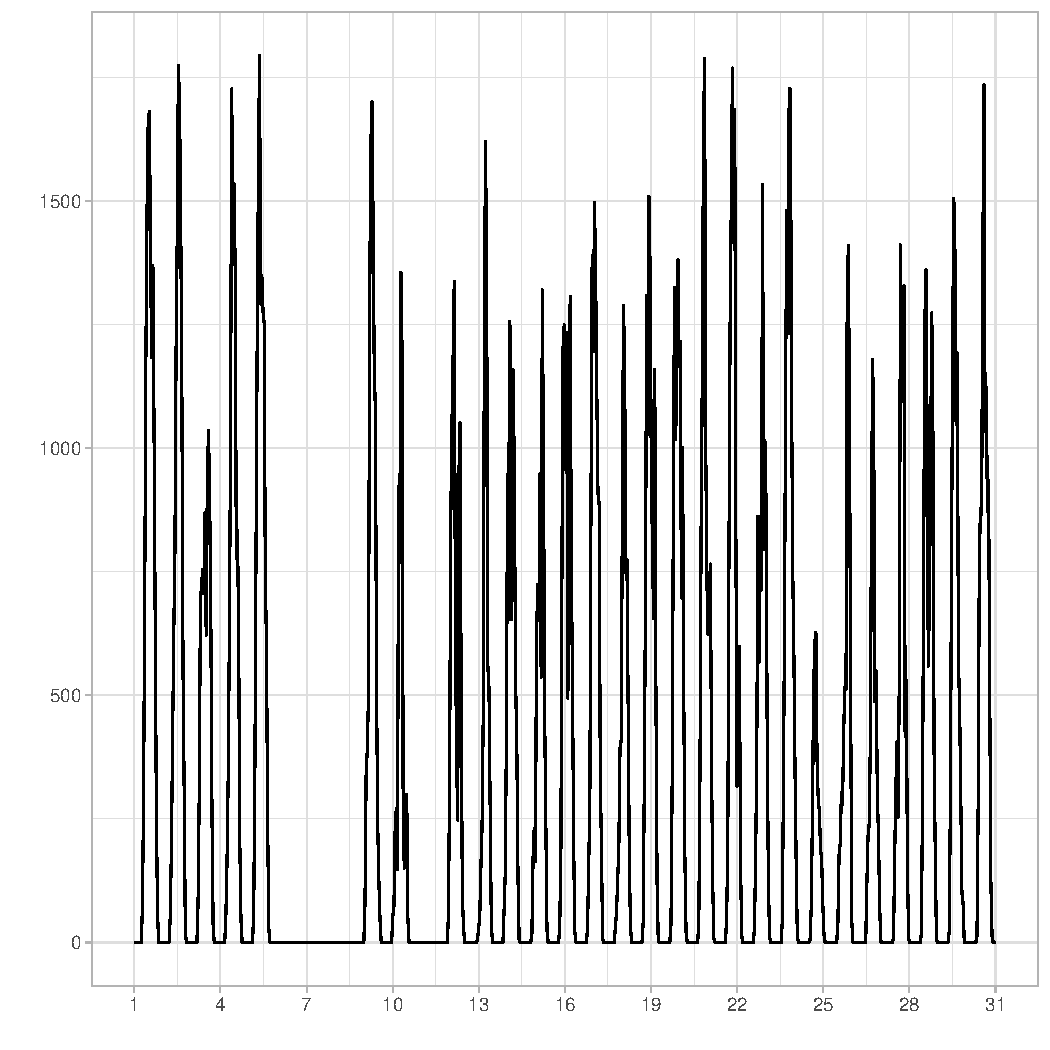
\includegraphics[width=.4\textwidth]{figR/ByDay.pdf} 
    &  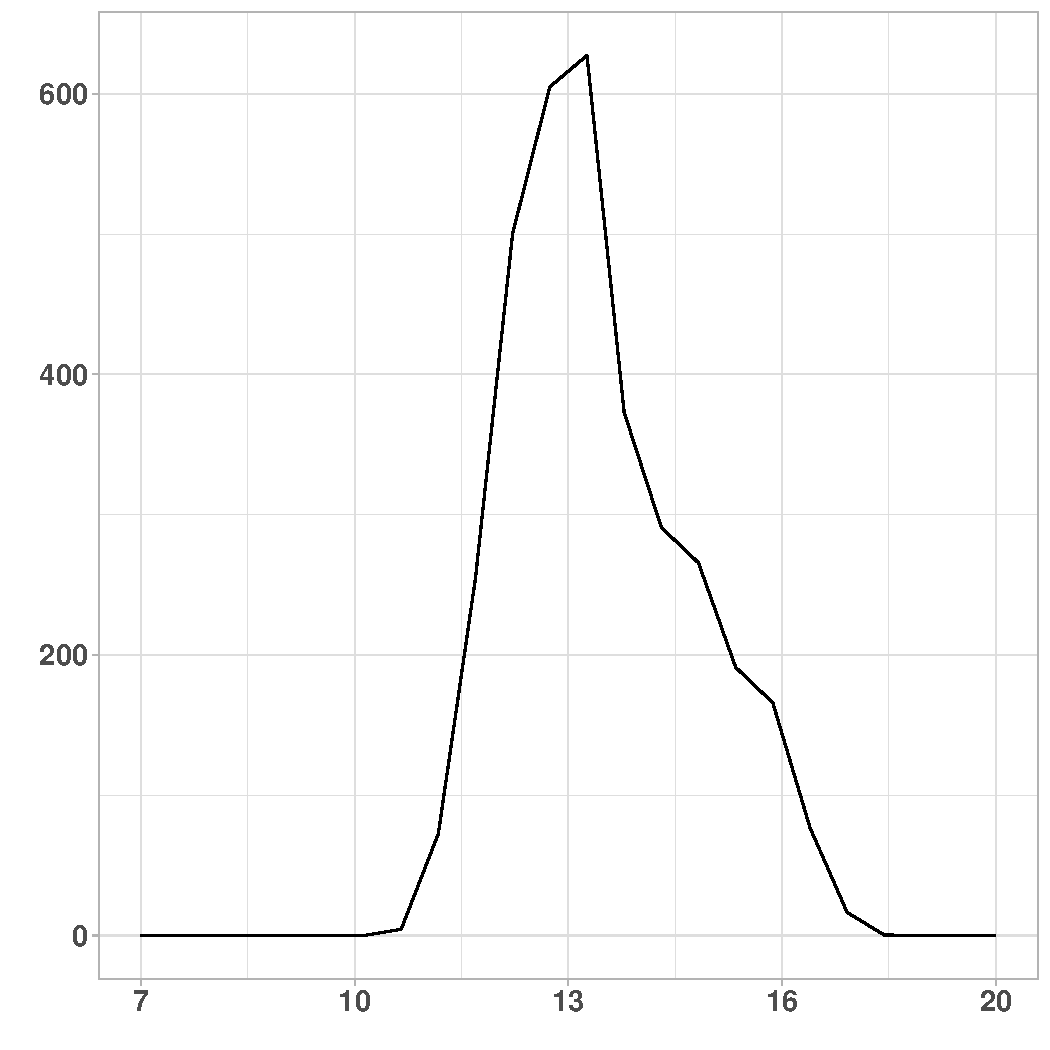
\includegraphics[width=.4\textwidth]{figR/HourDay.pdf}\\
    & Days & Hours \\
  \end{tabular}   
\caption{Power production by PVzen for August 2014 (left) and \\for August 25\textsuperscript{th} 2014 (right)}
\label{fig:PowerExample}
\end{center}
\end{figure}


\subsection{Estimation of the error}

So far, experts are using the code with some parameter values with the knowledge that these parameters are uncertain (the so called reference values). They can also provide more expertise on the nature of the parameter. For example for $a_r$, the nominal value is $0.17$ and experts state that the parameter lies within the $95\%$ confidence interval $[0.05,0.29]$. We chose to consider $a_r$ as Gaussian with $a_r\sim\mathcal{N}(\mu=0.17,\sigma^2=3.6.10^{-3})$. The standard deviation is chosen equal to $0.06$ because we have considered the upper bound and the lower bound of the given interval as respectively the quantiles $a_{r_{0.975}}$ and $a_{r_{0.025}}$. Similarly, $\eta$ and $\mu_t$ are taken as Gaussian such as $\eta\sim\mathcal{N}(\mu=0.143,\sigma^2=2.5.10^{-3})$ and $\mu_t\sim\mathcal{N}(\mu=-0.4,\sigma^2=10^{-2})$. If $100$ realizations are drawn from the joint distribution of $\eta$, $\mu_t$ and $a_r$, the production curve and the \textit{prior} credibility interval can be simultaneously plotted on a same graph to see how uncertain the predicted power is over a day. Figure \ref{fig:ParamError} illustrates on the left the distribution of $\eta$, $\mu_t$ and $a_r$ and on the right the production curve obtained for reference values and the \prior credibility interval at $90\%$. On the right side, experiments collected that same day are also displayed. One can check that the prior credibility interval, built thanks to the experts, looks coherent regarding the experimental data.\newline  


\begin{figure}[htbp!]
\centering
    \begin{tikzpicture}
		\tikzstyle{m1}=[]
		
		\node[m1] (N1) at (0,0) {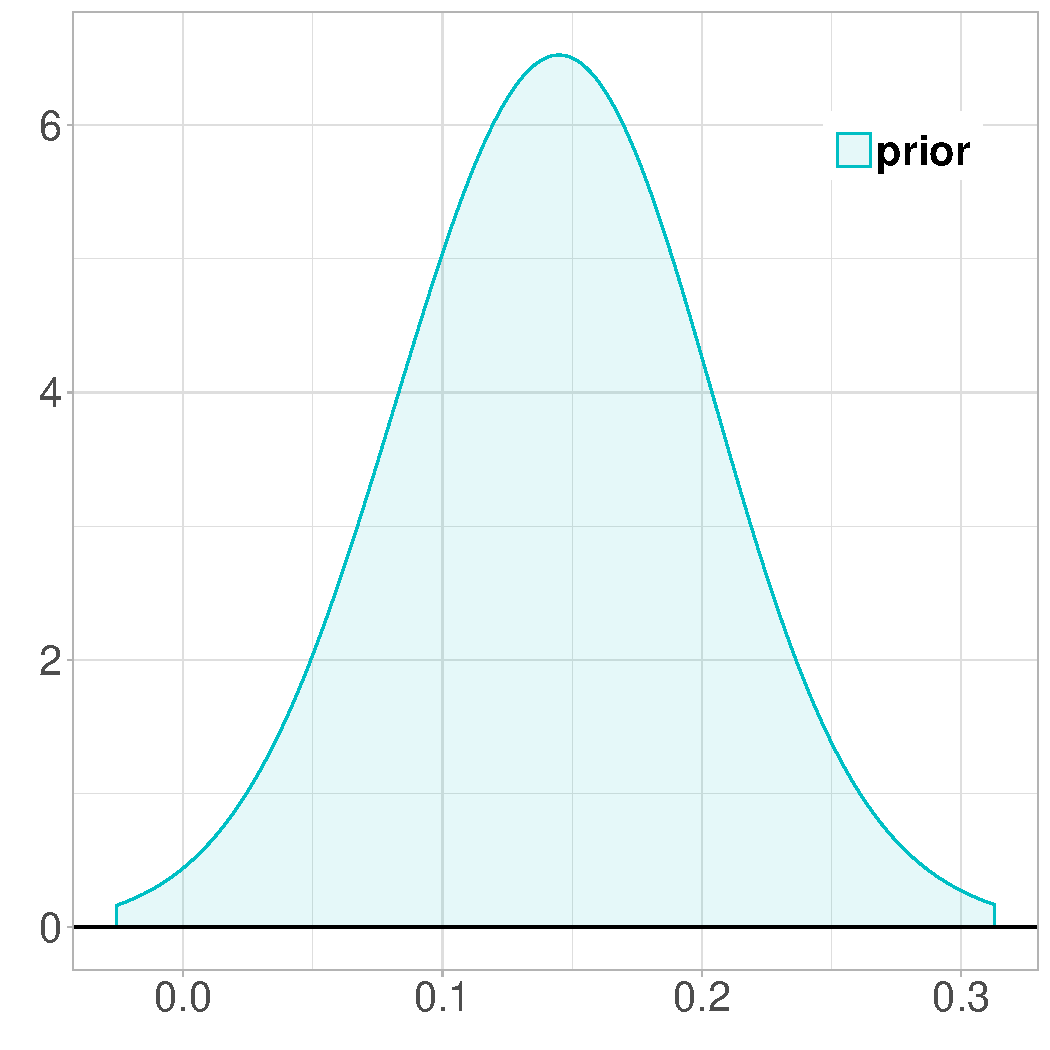
\includegraphics[width=.2\textwidth]{figR/densEta}};
		\node[m1] (N2) at (-1.7,0) {\rotatebox{90}{density}};
		\node[m1] (N3) at (0,-1.8) {$\eta$};
		\node[m1] (N11) at (-5.1,-2) {\rotatebox{90}{density}};
		\node[m1] (N10) at (-3.5,-2) {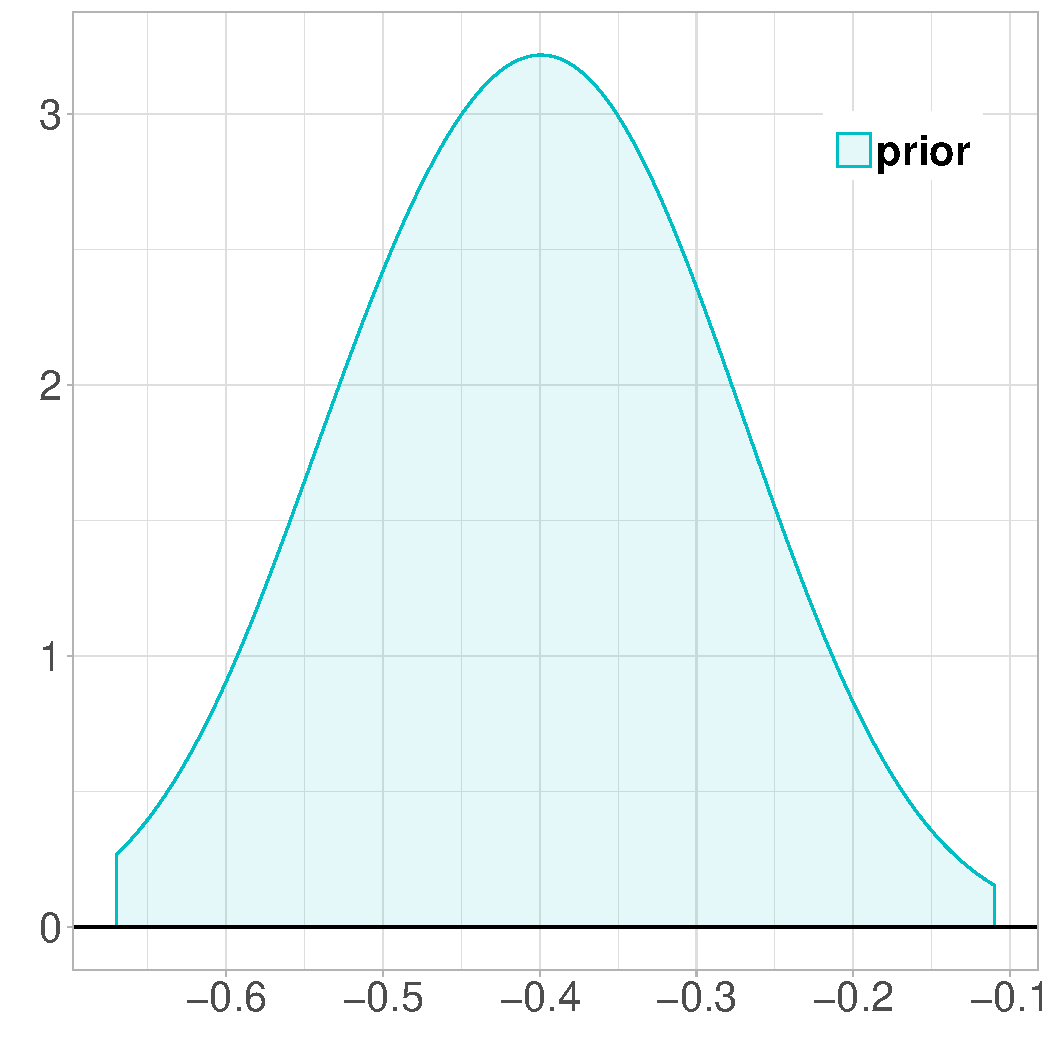
\includegraphics[width=.2\textwidth]{figR/densMu}};
		\node[m1] (N12) at (-3.5,-3.8) {$\mu_t$};
		\node[m1] (N9) at (-1.7,-4) {\rotatebox{90}{density}};
		\node[m1] (N4) at (0,-4) {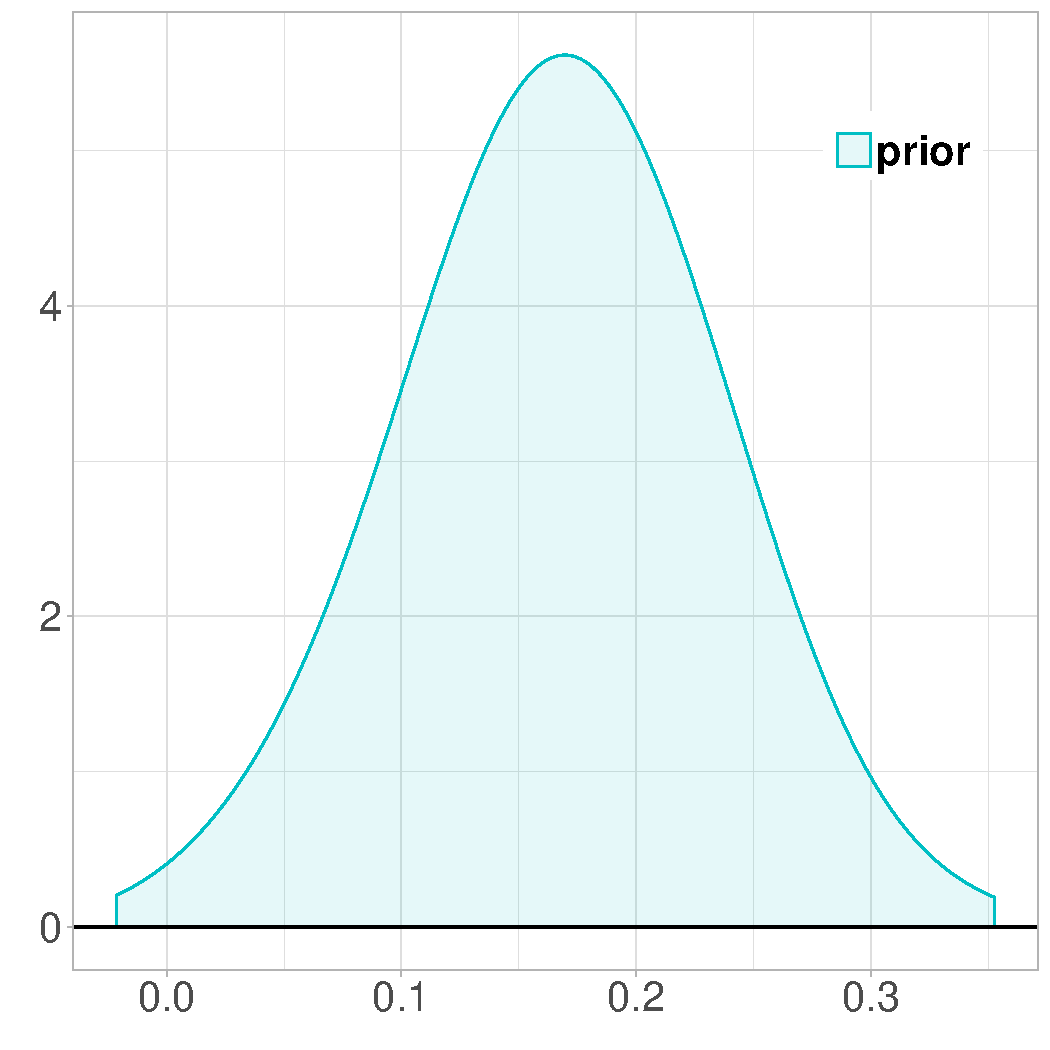
\includegraphics[width=.2\textwidth]{figR/densAr}};
		\node[m1] (N5) at (0,-5.8) {$a_r$};
		\node[m1] (N8) at (2.2,-2) {\rotatebox{90}{Power in $W$}};
		\node[m1] (N6) at (5.8,-2.1) {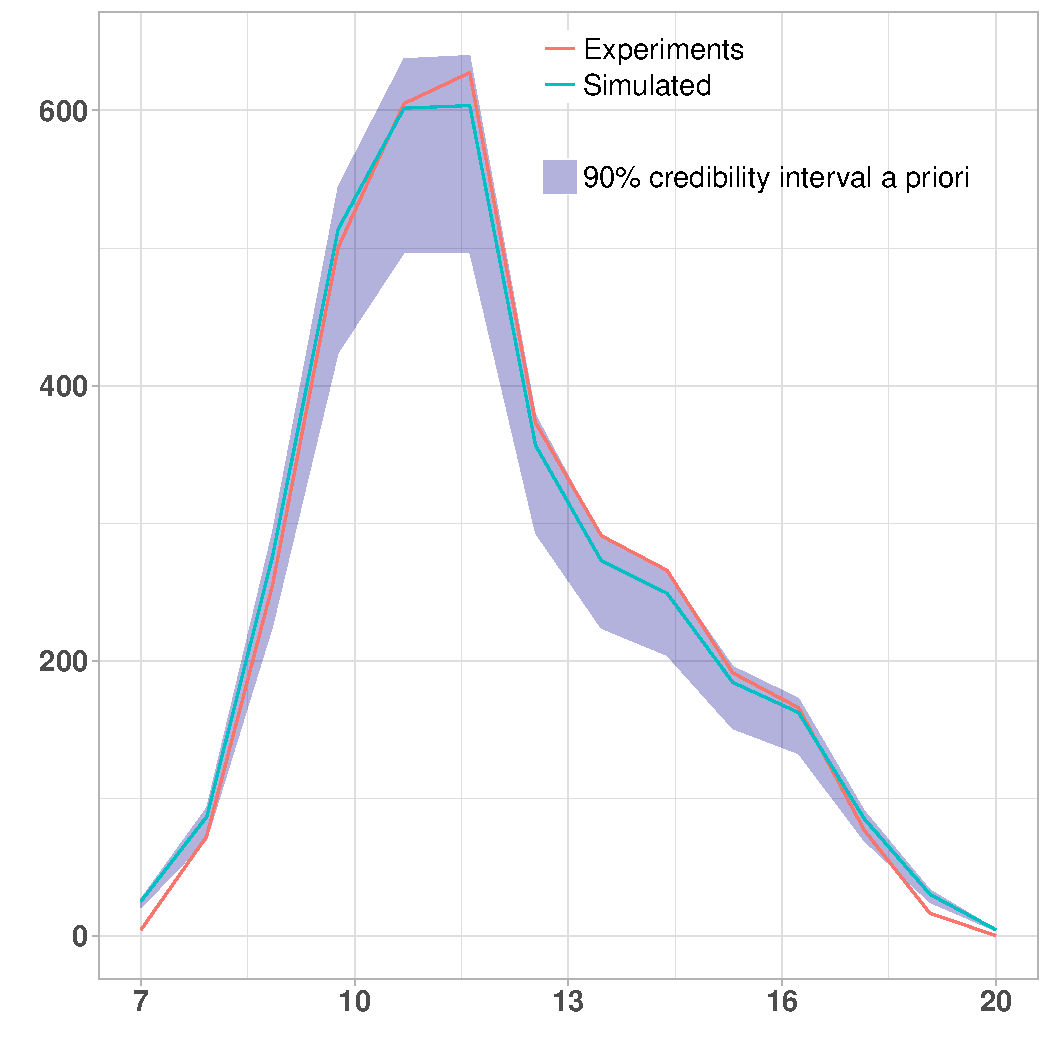
\includegraphics[width=.45\textwidth]{figR/credInterPrior.pdf}};
		\node[m1] (N7) at (5.8,-6) {Hours};
	
    \end{tikzpicture}
    
  \caption{$\pi(\eta)$, $\pi(\mu_t)$ and $\pi(a_r)$ prior densities (represented on the left panel) and induced credibility interval of the instantaneous power (right panel)}
  \label{fig:ParamError}
\end{figure}



If one is interested in the energy produced rather than the power (the energy in $kWh$ is the power in $kW$ multiplied by a duration), one can easily compute the maximum and the minimum energy for say $100$ realizations. The energy for collected power is $W_{exp}=3.44 kWh$, the maximum energy computed $W_{max}=3.65 kWh$ and the minimum energy $W_{min}=2.93 kWh$. Straightforwardly $W_{min} < W_{exp} < W_{max}$ which means that the experts interval seems correct for that day. With the considered uncertainty on $\eta$, $\mu_t$ and $a_r$, the error made is about $20\%$ over only one day. 
Considering this error over a day, cumulative error over a lifetime plant could be too prejudicial. The aim of the calibration is to quantify this error and, at the same time, increase the knowledge on the parameter distribution.
%If we consider this error as constant, cumulative error over a lifetime plant could be too prejudicial. The aim of the calibration is to decrease this error on the output. 
The results of calibration for this application case are detailed in Section \ref{sec:application}.


\section{Calibration through statistical models \label{sec:calibration}}

Calibration intends to find the ``best fitting'' parameters of a computational code, in order to minimize the difference between the output and the experiments. The variance of the measurement error is also unknown and has to be estimated as well as the parameters but will be considered as a nuisance parameter. It can be used in two cases. In a forecasting context \citep{craig2001}, where the calibrated code on data collected on site can be used to compute the behavior of the power plant over the next time period. But also, in a prediction context, where data from an experimental stand are used to predict the behavior of a non-existing stand (assuming they have the same features). \newline

A simple way to express calibration is to write down a first and straightforward model. The computational code is set up to entirely replace the physical system. Intuitively, we can assume that $\forall \boldsymbol{x} \in \mathcal{H}, \zeta(\boldsymbol{x})=f_c(\boldsymbol{x},\boldsymbol{\theta})$ for some well-chosen $\boldsymbol{\theta}$, which leads to the following equation\hc 

\begin{equation}
\mathcal{M}_1\ : \ \forall i \in \llbracket1,\dots,n\rrbracket \quad  y_{exp_i}=f_c(\boldsymbol{x}_i,\boldsymbol{\theta})+\epsilon_i,
\label{eq:model1}
\end{equation}

with $\forall i \in \llbracket1,\dots,n\rrbracket \quad \epsilon_i\overset{iid}{\sim}\mathcal{N}(0,\sigma_{err}^2)$.\newline


%The difficulties implied by such a model appear quickly. Indeed, to realize calibration, we need to compare for each candidate parameter value $\boldsymbol{\theta}$, the computer code output $f_c(\boldsymbol{x}_i,\boldsymbol{\theta})$ corresponding to each available observation $y_{exp_i}$.
%
%Actually, to estimate parameters, the maximum likelihood estimation could be a way to reach this purpose. To realize it, a lot of code calls are necessary. Especially in a Bayesian framework, where the update of a \prior  distribution with a likelihood is looked for, the number of runs are really important (straightforwardly linked to the number of runs in a Markov Chain Monte Carlo (MCMC) \cite{robert1996}). When the code is time-consuming, these methods become unrealistic. 

The likelihood of such a model is a function of $f_c$. In methods such as Maximum Likelihood Estimation (MLE) or as in Bayesian estimation (making recourse to many MCMC iterations), it becomes intractable to work with a time consuming $f_c$.\newline

For the sake of simplicity we will consider, in what follows, the code as deterministic. It means that for the same inputs, the output of the code is identical, which is generally the case. Even in a deterministic context, a gap between the code and the physical system is often unavoidable. This gap is called code error or discrepancy. Some papers advocate for adding this discrepancy in the statistical models \citep{kennedy2001,higdon2004,bayarri2007,bachoc2014}. In the following, we present three models which take into account a time consuming code and/or an additional discrepancy.
\newline

% Three different models are presented in the paper from this point which are conditioned by the issues mentioned above.
%
%Moreover, what is the legitimacy of the code regarding the physical system? Actually, a discrepancy often appears between the code and the physical system and has to be taken into account. Finally, a repetition of a code with same inputs could be different (stochastic code). For the sake of simplicity we will consider, for the rest of the article, the code as deterministic. We will therefore deal with the two remaining issues discussed above, which are: the code's computational complexity, and the presence of a discrepancy. These have motivated the development of several models which are described below. In this section, an overview of these models is given first. Then, the different likelihoods relative to each models will be detailed. Third, multiple ways to estimate the hyperparameters will be presented.

%In the first section, an overview of these models is given. The second section will deal with the establishment of the likelihood depending on the different model. The third section will highlight the multiple ways to estimate parameters. This will lead to the part where the models are tested in the frame of our application case and where choices are presented and explained.

\subsection{Presentation of the models}

\subsubsection{A time consuming code}

\noindent Let us consider a time consuming code. As said above, in this particular case, the computational burden become too huge to perform calibration. That is why, \citet{sacks1989} introduced an emulation of the, not yet computed, outputs from the code by a random function, \textit{i.e.} a stochastic process. The common choice is oriented toward the Gaussian process because the conditional Gaussian process is still a Gaussian process (see Appendix \ref{ap:GaussianProcesses} for more details). It is, parsimoniously, defined by its mean and covariance functions. The first ``simple'' and straightforward model was introduced by \citet{cox2001} which uses this emulation of $f_c$.

%An analytic form as a stochastic process would allow to compute this surrogate as many times as we want. A limited number of run of the time consuming code gives us simulated data and can help to design this surrogate. In \cite{sacks1989}, the stochastic process chosen is a Gaussian process defined by its mean and covariance functions (see the appendix \ref{ap:GaussianProcesses} for more details). 

\begin{eqnarray}
\mathcal{M}_2 \ : \ \forall i \in \llbracket1,\dots,n\rrbracket \quad y_{exp_i} &=& F(\boldsymbol{x}_i,\boldsymbol{\theta}) + \epsilon_i,
\label{eq:M2}\\
F(\bullet,\bullet) & \sim &{\mathcal{GP}}{\Big(m_S(\bullet,\bullet),c_S\{(\bullet,\bullet),(\bullet,\bullet)\}\Big)},
\nonumber
\end{eqnarray}
where $\forall i \in \llbracket1,\dots,n\rrbracket \quad \epsilon_i\overset{iid}{\sim}\mathcal{N}(0,\sigma_{err}^2)$ and the random function $F(\boldsymbol{x}_i,\boldsymbol{\theta})$ stands for a Gaussian process (GP) over the joint domain of $\boldsymbol{x}_i$ and $\boldsymbol{\theta}$. For the following, we consider that the measurement error is independent from the error made by the Gaussian process. The mean function $m_{S}(\boldsymbol{x}_i,\boldsymbol{\theta})$ is generally a linear form of simple functions of $\boldsymbol{x}_i$ and $\boldsymbol{\theta}$. Its covariance function $c_S\{(\boldsymbol{x}_i^*,\boldsymbol{\theta}^*),(\boldsymbol{x}_i,\boldsymbol{\theta})\}=\sigma_S^2 r_{\boldsymbol{\psi}_S}\{(\boldsymbol{x}_i^*,\boldsymbol{\theta}^*),(\boldsymbol{x}_i,\boldsymbol{\theta})\}$ is such as the function $r_{\boldsymbol{\psi_S}}\{(\bullet,\bullet),(\bullet,\bullet)\}$ is the correlation function with a vector parameter $\boldsymbol{\psi}_S$. This parameter vector represents the scale and the regularity of the kernel and where $\sigma_S^2$ represents the variance. The mean $m_{S}(\boldsymbol{x}_i,\boldsymbol{\theta})$ can be written as\newline




\begin{equation}
m_S(\boldsymbol{x}_i,\boldsymbol{\theta})=m_{\boldsymbol{\beta}_S}(\boldsymbol{x}_i,\boldsymbol{\theta})=\mathbb{E}[F(\boldsymbol{x}_i,\boldsymbol{\theta})]=\beta_{S_0}+\sum_{j=1}^{M}\beta_{S_j}h_{S_j}(\boldsymbol{x}_i,\boldsymbol{\theta})=\boldsymbol{h}_S(\boldsymbol{x}_i,\boldsymbol{\theta})\boldsymbol{\beta}_S,
\label{eq:MeanLin}
\end{equation}

where $\boldsymbol{\beta}_S^T=(\beta_{S_0},\dots,\beta_{S_M})$ is the coefficient vector to be estimated and $\boldsymbol{h}_S(\bullet,\bullet)=(h_{S_0}(\bullet,\bullet),\dots\allowbreak,h_{S_M}(\bullet,\bullet))$ the row vector of regression functions where $h_{S_0}=1$. Similarly, we define the $n\times(M+1)$ matrix $\boldsymbol{H}_{S}(\boldsymbol{X},\boldsymbol{\theta})$ such as its $i^{th}$ row is $\boldsymbol{h}_{S}(\boldsymbol{x}_i,\boldsymbol{\theta})$. The correlation function can take multiple forms as Gaussian or Matérn for instance \citep[see][for more examples]{santner2013}.
We will consider, for now and for all theoretical developments, the general form of $c_S\{(\bullet,\bullet),(\bullet,\bullet)\}=\sigma_S^2 r_{\boldsymbol{\psi}_S}\{(\bullet,\bullet),(\bullet,\bullet)\}$ where $\sigma_S^2$ is the variance and $r$ is the correlation function with a parameter vector $\boldsymbol{\psi}_S$. The advantage of using a surrogate model, for $f_c(\boldsymbol{X},\boldsymbol{\theta})$ is to alleviate the computational burden, at the cost of adding an additional source of uncertainty, and of increasing the number of uncertain parameters. Specific hypotheses, for instance a known smoothness of the random field, may help to choose the size of the parametric family in which the correlation
shape is to be assessed. 
% We will see for the application case how such choices can impact the results. \PB{le fait on vraiment ?}\MCC{Non, tu as raison. On fixe des hypothèses au départ que l'on teste mais on ne va en aucun cas tester les effets des changements des noyaux ou des autres hypothèses.}
\newline

When the code is time consuming, a fixed number $N$ of simulations is set up. The ensuing simulated data (we will call them $\boldsymbol{y}_c$) are usually the image of a design of experiments (DOE) representative of the input space. Some interesting developments have been made on using the least possible points in the input space with some wise repartitions (the \textit{Latin Hilbert Space} sampling is one example, some good insights are available in \citet{pronzato2012}). \newline

% \PB{il faut préciser à un moment que l'input space est le produit entre l'espace des x et des theta}
Let us call $\boldsymbol{D}$ a DOE, a set of $N$ points sampled in the input space defined as the product of $\mathcal{H}$ and $\mathcal{Q}$. We can write $\boldsymbol{D}=\{ (\boldsymbol{x}_1^D,\boldsymbol{\tau}_1^D),\dots (\boldsymbol{x}_N^D,\boldsymbol{\tau}_N^D) \}$ where $\forall i \in \llbracket1,\dots,N\rrbracket \  (\boldsymbol{x}_i^D,\boldsymbol{\tau}_i^D)$ are chosen in $\mathcal{H}\times \mathcal{Q}$.
% where $(\boldsymbol{\tau}_1^D,\dots,\boldsymbol{\tau}_N^D)$ is a set of $N$ vectors chosen accordingly to the DOE design in the input space parameter $\mathcal{Q}$. 
The establishment of the DOE will lead to simulated data which are defined as $\boldsymbol{y}_c=f_c(\boldsymbol{D})$. The error made by the surrogate strongly depends on the numerical design of experiments used to fit the emulator. Adaptive numerical designs introduced in \citet{damblin2018} is a way to enhance the emulator when the goal is to calibrate the code. This method, based on a Gaussian process-based optimization called Efficient Global Optimization \citep{jones1998efficient}, allows to add, wisely regarding further calibration, another points in the original DOE. \newline

% The aim is to use these $N$ points and the $n$ experimental points for estimating the parameters of the Gaussian process.\newline

\subsubsection{With a code error}

\noindent Considering the computational code as a perfect representation of the physical system may be a too strong hypothesis and it is legitimate to wonder whether the code might differ from the phenomenon. This error (called discrepancy and introduced above) can be defined as\hc
%This error (also called code error or discrepancy) has been introduced in many papers \citep{kennedy2001,bayarri2007,higdon2004} in a calibration framework. The definition of this term seems straightforward\hc
\begin{equation*}
\delta(\boldsymbol{x}_i)=\zeta(\boldsymbol{x}_i)-f_c(\boldsymbol{x}_i,\boldsymbol{\theta}).
\end{equation*}
In all the works cited above, this unknown discrepancy is modeled as a realization of a Gaussian process, this time yielding a random function over the domain of $\boldsymbol{X}$ variables only. For the sake of simplicity we will denote by $m_s$, $c_S$ ($c_{\sigma_S^2,\boldsymbol{\psi}_S}$) and $r_S$ ($r_{\boldsymbol{\psi}_S}$) the mean, covariance (with $\sigma_S^2$ as the variance) and correlation function relative to the surrogate and by $m_{\boldsymbol{\delta}}$, $c_{\boldsymbol{\delta}}$ ($c_{\sigma_{\boldsymbol{\delta}}^2,\boldsymbol{\psi}_{\boldsymbol{\delta}}}$) and $r_{\boldsymbol{\delta}}$ ($r_{\boldsymbol{\psi}_{\boldsymbol{\delta}}}$) the same functions relative to the discrepancy (respectively $\sigma_{\boldsymbol{\delta}}^2$ for the variance in the covariance function). 
Note that $m_{\boldsymbol{\delta}}$ and $c_{\boldsymbol{\delta}}$ are functions of $\boldsymbol{x}$ only and not $\boldsymbol{\theta}$. The aim of adding the discrepancy lies in the fact that correlation is sometimes visible in the residuals and/or that no value of $\boldsymbol{\theta}$ makes the computer close to experiments. However, the discrepancy could lead to an identifiability issue. For example, it could easily exist two couples $(\boldsymbol{\theta},\delta(\boldsymbol{x}_i))$ and $(\boldsymbol{\theta}^*,\delta^*(\boldsymbol{x}_i))$ that verify the two equalities\hc $\delta(\boldsymbol{x}_i)=\zeta(\boldsymbol{x}_i)-f_c(\boldsymbol{x}_i,\boldsymbol{\theta})$ and $\delta^*(\boldsymbol{x}_i)=\zeta(\boldsymbol{x}_i)-f_c(\boldsymbol{x}_i,\boldsymbol{\theta}^*)$. Some papers \citep{higdon2004,bachoc2014,bayarri2007} advocate to set the mean of the discrepancy to 0 to solve this identifiability issue. The contribution of the discrepancy is widely discussed in literature and make the object of comparative studies in validation \citep{damblin2015}. \newline



When the code is not time consuming, the real code $f_c$ is used\hc

\begin{eqnarray}
\mathcal{M}_3 \ : \ \forall i \in \llbracket1,\dots,n\rrbracket \quad y_{exp_i}&=& f_c(\boldsymbol{x}_i,\boldsymbol{\theta})+\delta(\boldsymbol{x}_i)+\epsilon_i,
\label{eq:M3}\\
\delta(\bullet) & \sim &{\mathcal{GP}}{\Big(\boldsymbol{m}_{\delta}(\bullet),c_{\delta}(\bullet,\bullet)\Big)},
\nonumber
\end{eqnarray}

where $\forall i \in \llbracket1,\dots,n\rrbracket \quad \epsilon_i\overset{iid}{\sim}\mathcal{N}(0,\sigma_{err}^2)$, and $\delta(\bullet)$ stands for a Gaussian process which mimics the discrepancy and will only depends on the input variables $\boldsymbol{x}$. For the rest of the article, we make the assumption that the discrepancy is independent from the measurement error. We can write $\delta(\bullet)\sim\mathcal{GP}(\boldsymbol{m}_{\delta}(\bullet),c_{\delta}(\bullet,\bullet))$ with $\forall \boldsymbol{x}, \ \boldsymbol{m}_{\delta}(\boldsymbol{x})={\boldsymbol{h}_{\delta}}(\boldsymbol{x})\boldsymbol{\beta}_{\delta}$ (where $\boldsymbol{h}_{\delta}$ is a row vector and $\boldsymbol{\beta}_{\delta}$ is a column vector if we choose a parametric representation of the mean) and $c_{\delta}$ the covariance function of the discrepancy. We also denote $\boldsymbol{H}_{\delta}(\boldsymbol{X})$ the $n$ row matrix, the $i^{th}$ row of which is $\boldsymbol{h}_{\delta}(\boldsymbol{x}_i)$.\newline

When the code is time consuming, the systematic use of $f_c$ is not computationally acceptable.
Then, as for Model $\mathcal{M}_2$, the code is replaced with a Gaussian process. This leads to the more generic model introduced in \citet{kennedy2001}.

% 
% The replacement of the, not yet computed, values of $f_c$ by a Gaussian process may bring a bias and has to be taken
% into account into the statistical model. The more generic model has been introduced in \citet{kennedy2001}. 
% Model $\mathcal{M}_4$ remains close to $\mathcal{M}_3$.

\begin{equation}
\mathcal{M}_4 \ : \ \forall i \in \llbracket1,\dots,n\rrbracket \quad y_{exp_i}= F(\boldsymbol{x}_i,\boldsymbol{\theta})+\delta(\boldsymbol{x}_i)+\epsilon_i,
\label{eq:M3p}
\end{equation}
where $\forall i \in \llbracket1,\dots,n\rrbracket \quad \epsilon_i\overset{iid}{\sim}\mathcal{N}(0,\sigma_{err}^2)$, $F(\boldsymbol{x}_i,\boldsymbol{\theta})$ and $\delta(\boldsymbol{x}_i)$ are two Gaussian
processes defined as before. Similarly than before, we consider, for the following, that the measurement error, the discrepancy and the error induced by the surrogate are all independent.
In their model, \citet{kennedy2001} also used a scale parameter $\rho$ in front of $F$.
This parameter is usually set to $1$ in many works  in order to achieve the best estimate on $\boldsymbol{\theta}$.
Thus, we omit this parameter in the model definition.
\newline

%The assumption to take, the multiplicative bias, $\rho$ as constant seems natural and follows if $F(\bullet,\bullet)$, $\delta(\bullet)$, and $\zeta(\bullet)$ are stationary processes \citep{kennedy2001}. Mainly the mean function of the discrepancy is considered linear and the particular case of $\rho=1$ is introduced in \citet{bayarri2007}. We will consider for the rest of the article $\rho=1$.
A quantification of the bias form is the aim of both models. If we are interested in improving the computational code or its surrogate, it is usually fair to set the mean of the discrepancy to zero and find the best tuning parameter vector which compensates a potential bias \citep{higdon2004,bachoc2014}. \newline

\begin{figure}[htbp!]
  \centering
	
    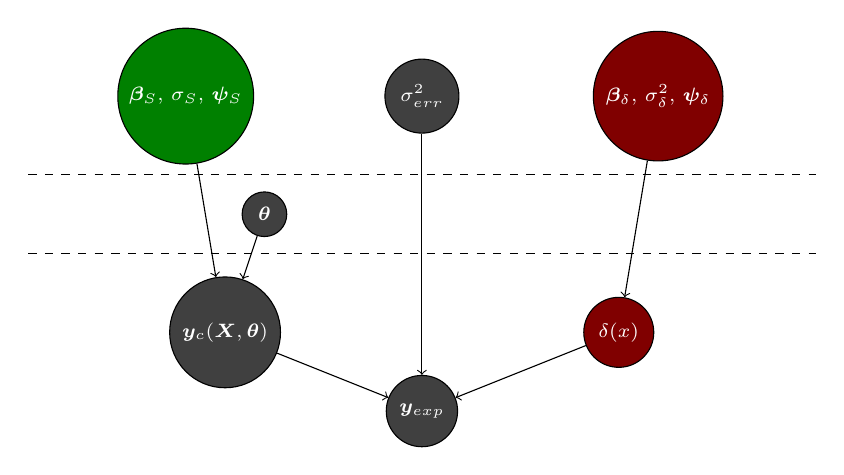
\begin{tikzpicture}
		\tikzstyle{m1}=[fill=gray!50!black, text=white,font=\scriptsize, circle,draw]
		\tikzstyle{m2}=[fill=red!50!black,text=white,font=\scriptsize, circle, draw]
		\tikzstyle{m3}=[fill=blue!50!black, text=white, font=\scriptsize, circle, draw]
		\tikzstyle{m4}=[fill=green!50!black, text= white, font=\scriptsize, circle, draw]
		
		\node[m1] (N1) at (0,0) {$\boldsymbol{y}_{exp}$};
		\node[m1] (N2) at (-2.5,1) {$\boldsymbol{y}_c(\boldsymbol{X},\boldsymbol{\theta})$};
		\node[m1] (N3) at (0,4) {$\sigma_{err}^2$};
		\node[m1] (N4) at (-2,2.5) {$\boldsymbol{\theta}$};
		\node[m2] (N5) at (3,4) {$\boldsymbol{\beta}_\delta$, $\sigma_\delta^2$, $\boldsymbol{\psi}_\delta$};

		\node[m4] (N7) at (-3,4) {$\boldsymbol{\beta}_S$, $\sigma_S$, $\boldsymbol{\psi}_S$};
		\node[m2] (N8) at (2.5,1) {$\delta(x)$};

		\draw [->] (N2) to (N1);
		\draw [->] (N3) to (N1);
		\draw [->] (N4) to (N2);
		\draw [->] (N7) to (N2);
		\draw [->] (N5) to (N8);
		\draw [->] (N8) to (N1);		
		
		\draw [dashed] (-5,3) to (5,3);
		\draw [dashed] (-5,2) to (5,2);
		
		
    \end{tikzpicture}
    
  \caption{Directed Acyclic Graph (DAG) representation of the different models}
  \label{fig:DAG}
\end{figure}


Figure \ref{fig:DAG} is a summary of all the models introduced above. The directed acyclic graph (DAG) allows us to compare the structures of all the previously introduced models. 
Specifically\hc if one considers only the grey nodes, the obtained DAG corresponds to Model $\mathcal{M}_1$. Adding the green node, the resulting DAG represents $\mathcal{M}_2$. Considering the grey and red nodes, yields a DAG for model $\mathcal{M}_3$ and the whole DAG represents the general model $\mathcal{M}_4$. Note that two categories of parameters are considered. The tuning parameters are only related to the code and other parameters (also called nuisance parameter) concern the measurement error, the surrogate or the discrepancy introduced in the models. In calibration, we only focus on the value of $\boldsymbol{\theta}$ but the other parameters introduced need to be estimated as well. We will dig into these estimation issues in Section \ref{sec:estimation}.\newline

All these models introduce new parameters and need to be estimated as well as tuning parameters. Estimation needs to dive into technical aspects such as writing the likelihood for each model. The following section provides all the elements required to go one step further and carry out estimation. \newline


\subsection{Likelihood}


For estimating parameters (whatever framework used, Bayesian or Maximization Likelihood Estimation (MLE)), expressing the likelihood comes as the first requirement. Two major categories stand out. When the code is not time consuming, the main issue in code calibration (\textit{i.e.} the computational time burden) is avoided. When the code is time consuming, new parameters have to be taken into account and to be estimated. In the models $\mathcal{M}_2$ and $\mathcal{M}_4$, numerical data ($\boldsymbol{y}_c$) as much as field data ($\boldsymbol{y}_{exp}$) and can be collected into the whole data vector $\boldsymbol{y}^T=(\boldsymbol{y}_{exp}^T,\boldsymbol{y}_c^T)$. Then, in the models $\mathcal{M}_1$ and $\mathcal{M}_3$, data can only represent field data ($\boldsymbol{y}_{exp}$).
In what follows, we will denote by $\boldsymbol{\theta}^*$ the true parameter vector.
Note that it is well-defined only in Models~$\mathcal{M}_1$ and $\mathcal{M}_2$, as the value of $\boldsymbol{\theta}$ which satisfies\hc $\zeta(\boldsymbol{x})=f_c(\boldsymbol{x},\boldsymbol{\theta}^*)$ for all possible $\boldsymbol{x}$, (assuming such a $\boldsymbol{\theta}$ exists and is unique). On the other hand, the models $\mathcal{M}_3$ and $\mathcal{M}_4$ are both defined by the relation $\zeta(\boldsymbol{x})=f_c(\boldsymbol{x},\boldsymbol{\theta})+\delta(\boldsymbol{x})$, which holds for infinitely many couples $(\boldsymbol{\theta},\delta(\bullet))$, as discussed earlier. \citet{kennedy2001} avoid this issue by defining $\boldsymbol{\theta}^*$ as a ``best-fitting'' value, but it is unclear what this means exactly (see the discussion section of their paper for further details).\newline
%Let $D_{exp}(\boldsymbol{X})=\{\boldsymbol{x}_1,\dots,\boldsymbol{x}_n\}$ denote the set of input variables and $D_{exp}(\boldsymbol{X},\boldsymbol{\theta})=\{(\boldsymbol{x}_1,\boldsymbol{\theta}),\dots,(\boldsymbol{x}_n,\boldsymbol{\theta})\}$ denote the input variables extended with the parameter values, both corresponding to experimental data. \newline

%To simplify the number of parameter to deal with,

In order to simplify the notation, we will use for the rest of the paper $\Phi=\{\sigma_S^2,\sigma_{\delta}^2,\boldsymbol{\psi}_S,\boldsymbol{\psi}_{\delta}\}$ and $\Phi_S=\{\sigma_S^2,\boldsymbol{\psi}_S\}$ and $\Phi_{\delta}=\{\sigma_{\delta}^2,\boldsymbol{\psi}_{\delta}\}$, where $\sigma_S^2$ and $\sigma_{\delta}^2$ are the variances of the two Gaussian processes respectively relative to the surrogate and the discrepancy. The two parameter vectors $\boldsymbol{\psi}_S$ and $\boldsymbol{\psi}_{\delta}$ are relative to the correlation functions. Let us call $\boldsymbol{\beta}^T=(\boldsymbol{\beta}_S^T,\boldsymbol{\beta}_{\delta}^T)$ the vector of collected coefficient vectors.\newline

Both cases of time consuming or not time consuming code will be dealt with. The likelihood equations will be written for the generic forms of $\mathcal{M}_3$ and $\mathcal{M}_4$. The likelihoods for the simpler models
$\mathcal{M}_1$ and $\mathcal{M}_2$ 
will be then derived since  
$\mathcal{M}_1\subset\mathcal{M}_3$ and $\mathcal{M}_2\subset\mathcal{M}_4$.\newline

\subsubsection{A fast code}

\noindent The generic model which deals with calibration with a code quick to run is detailed in \EqRef{eq:M3}. Experimental data are the only one needed because simulation data are free but will not bring additional information for the parameters of Model $\mathcal{M}_3$.
Experimental data follow a Gaussian distribution, the expectation of which
is\hc \newline

\begin{equation*}
\mathbb{E}[\boldsymbol{y}_{exp}|\boldsymbol{\theta},\boldsymbol{\beta}_{\delta};\boldsymbol{X}] = \boldsymbol{m}_{exp}^{\boldsymbol{\beta}_{\delta}}(\boldsymbol{X},\boldsymbol{\theta}) = \boldsymbol{m}_{exp}(\boldsymbol{X},\boldsymbol{\theta}) = f_c(\boldsymbol{X},\boldsymbol{\theta}) + {\boldsymbol{H}_{\delta}}(\boldsymbol{X})\boldsymbol{\beta}_{\delta}.
\end{equation*}

Then, the expression of the variance is given by\hc

\begin{equation*}
\mathbb{V}ar[\boldsymbol{y}_{exp}|\Phi_{\delta};\boldsymbol{X}] = \boldsymbol{V}_{exp}^{\Phi_{\delta},\sigma_{err}^2}(\boldsymbol{X})= \boldsymbol{V}_{exp}(\boldsymbol{X}) = \boldsymbol{\Sigma}_{\delta}(\boldsymbol{X}) + \sigma_{err}^2\boldsymbol{I}_n,
\end{equation*}

with $\forall (i,j) \in \llbracket1,\dots,n\rrbracket^2: (\boldsymbol{\Sigma}_{\delta}(\boldsymbol{X}))_{i,j} =(\boldsymbol{\Sigma}^{\Phi_{\delta}}_{\delta}(\boldsymbol{X}))_{i,j}= c_{\delta}(\{\boldsymbol{x}_i,\boldsymbol{x}_j\})$. 
%\PB{mais $\delta$ discrepance ne dépend pas de $\theta$ non ??}
The likelihood in this particular case can be written as

\begin{equation}
\begin{split}
\mathcal{L}^{F}(\boldsymbol{\theta},\boldsymbol{\beta}_{\delta},\Phi_{\delta};\boldsymbol{y}_{exp},\boldsymbol{X})=\frac{1}{(2\pi)^{n/2}|\boldsymbol{V}_{exp}(\boldsymbol{X})|^{1/2}}\exp\Bigg\{-\frac{1}{2}\Big(\boldsymbol{y}_{exp}-\boldsymbol{m}_{exp}(\boldsymbol{X},\boldsymbol{\theta})\Big)^T\boldsymbol{V}_{exp}(\boldsymbol{X})^{-1}\\
\Big(\boldsymbol{y}_{exp}-\boldsymbol{m}_{exp}(\boldsymbol{X},\boldsymbol{\theta})\Big)\Bigg\}.
\end{split}
\label{eq:LikelihoodQuick2}
\end{equation}

This likelihood is relative to Model $\mathcal{M}_3$ (\EqRef{eq:M3}). For the specific case, where no discrepancy is considered (corresponding to $\mathcal{M}_1$ \EqRef{eq:model1}) the likelihood can be written in a similar way but with $\boldsymbol{m}_{exp}(\boldsymbol{X},\boldsymbol{\theta})= f_c(\boldsymbol{X},\boldsymbol{\theta})$ and $\boldsymbol{V}_{exp}(\boldsymbol{X})=\sigma_{err}^2\boldsymbol{I}_n$. Note that the covariance matrix depends only on $\sigma_{err}^2$. It implies that if we seek to estimate the \posterior density on $\boldsymbol{\theta}$ (in a Bayesian framework), this covariance term is superfluous.\newline


Then the likelihood can be rewritten in an simpler way\hc

\begin{equation}
\mathcal{L}^F(\boldsymbol{\theta},\sigma_{err}^2;\boldsymbol{y}_{exp},\boldsymbol{X})=\frac{1}{(2\pi)^{n/2}\sigma_{err}^{n}}\exp\Bigg\{-\frac{1}{2\sigma_{err}^2}||\boldsymbol{y}_{exp}-f_c(\boldsymbol{X},\boldsymbol{\theta})||_2^2\Bigg\}.
\label{eq:LikelihoodQuick}
\end{equation}

The models using the code with or without the discrepancy do look quite similar. For theoretical development, it might be easier to work with the one without discrepancy. From an experimental point of view, it could be interesting to study the role of the code error. \newline
%When the code turns out to be time consuming, the likelihoods relative to the models with Gaussian Processes surrogates become more complicated because the code $f_c$, itself, becomes a random object.\newline

\subsubsection{A time consuming code}

\noindent When a code is time consuming and replaced by a surrogate, additional parameters are to be estimated. As introduced above, a DOE is set up and intends to be a representative sample of the input space (variable and parameter input space). Simulated data from this DOE (called $\boldsymbol{y}_c$) will constitute additional data for the estimation of the nuisance parameters. Depending on how we consider that two sources of data are linked, 
multiple likelihoods can be set up. For the theoretical development, we will consider the general model $\mathcal{M}_4$ and we will detail the particular case $\mathcal{M}_2$ hereafter.\newline

%%%%%%%%%%%%%%%%%%%    Full likelihood

The first likelihood useful in estimation is the full likelihood. This one concerns the distribution of all collected data ($\boldsymbol{y}^T=(\boldsymbol{y}_{exp}^T,\boldsymbol{y}_c^T)$). That means, we are interested in estimating the parameters of the distribution $\pi(\boldsymbol{y}|\boldsymbol{\theta},\boldsymbol{\beta},\Phi,\sigma_{err}^2;\boldsymbol{X},\boldsymbol{D})$ which is Gaussian.
The expectations can be written from both expectancies of $\pi(\boldsymbol{y}_{exp}|\boldsymbol{\theta},\boldsymbol{\beta},\Phi,\sigma_{err}^2;\boldsymbol{X})$ and $\pi(\boldsymbol{y}_c|\boldsymbol{\theta},\boldsymbol{\beta}_S,\Phi_S;\boldsymbol{D})$.

\begin{equation}
\begin{cases}
    \mathbb{E}[\boldsymbol{y}_c|\boldsymbol{\beta}_S;\boldsymbol{D}]= \boldsymbol{m}_S^{\boldsymbol{\beta}_S}(\boldsymbol{D})= \boldsymbol{m}_S(\boldsymbol{D}) = {\boldsymbol{H}_S}(\boldsymbol{D})\boldsymbol{\beta}_S\\
\mathbb{E}[\boldsymbol{y}_{exp}|\boldsymbol{\theta},\boldsymbol{\beta};\boldsymbol{X}]= \boldsymbol{m}_{exp}^{\boldsymbol{\beta}}(\boldsymbol{X},\boldsymbol{\theta}) = \boldsymbol{m}_{exp}(\boldsymbol{X},\boldsymbol{\theta}) = {\boldsymbol{H}_S}(\boldsymbol{X},\boldsymbol{\theta}) \boldsymbol{\beta}_S + {\boldsymbol{H}_{\delta}}(\boldsymbol{X})\boldsymbol{\beta}_{\delta}
\end{cases}
\label{eq:ExpPartialLikelihood}
\end{equation}

%
%\begin{equation}
%\mathbb{E}[\boldsymbol{y}_c|\boldsymbol{\theta},\boldsymbol{\beta}_1,\Phi_1]= \boldsymbol{m}_c =\rho {\boldsymbol{H}_1}(D)\boldsymbol{\beta}_1
%\label{eq:ExpPartialLikelihood}
%\end{equation}
%and,
%
%\begin{equation*}
%\mathbb{E}[\boldsymbol{y}_{exp}|\boldsymbol{\theta},\boldsymbol{\beta},\Phi]=\rho {\boldsymbol{H}_1}(D_{exp}(\boldsymbol{\theta})) \boldsymbol{\beta}_1 + {\boldsymbol{H}_2}(D_{exp})\boldsymbol{\beta}_2
%\end{equation*}

This can be summed up for two component vectors $\boldsymbol{y}^T=(\boldsymbol{y}_{exp}^T,\boldsymbol{y}_c^T)$\hc
 
\begin{equation}
\begin{split}
\mathbb{E}[\boldsymbol{y}|\boldsymbol{\theta},\boldsymbol{\beta};\boldsymbol{X},\boldsymbol{D}]=\boldsymbol{m}_{\boldsymbol{y}}^{\boldsymbol{\beta}}((\boldsymbol{X},\boldsymbol{\theta}),\boldsymbol{D}) = \boldsymbol{m}_{\boldsymbol{y}}((\boldsymbol{X},\boldsymbol{\theta}),\boldsymbol{D})& =\boldsymbol{H}((\boldsymbol{X},\boldsymbol{\theta}),\boldsymbol{D})\boldsymbol{\beta}\\&=\begin{pmatrix}
\boldsymbol{H}_S(\boldsymbol{X},\boldsymbol{\theta}) & \boldsymbol{H}_{\boldsymbol{\delta}}(\boldsymbol{X})\\
\boldsymbol{H}_S(\boldsymbol{D}) & 0
\end{pmatrix}\boldsymbol{\beta}.
\end{split}
\label{eq:MeanFullLikelihood}
\end{equation}
The variance matrix now includes the covariance functions of the discrepancy and the surrogate.

\begin{equation}
\begin{split}
\mathbb{V}ar[\boldsymbol{y}|\boldsymbol{\theta},\Phi,\sigma_{err}^2;\boldsymbol{X},\boldsymbol{D}]&=\boldsymbol{V}^{\Phi,\sigma_{err}^2}((\boldsymbol{X},\boldsymbol{\theta}),\boldsymbol{D})=\boldsymbol{V}((\boldsymbol{X},\boldsymbol{\theta}),\boldsymbol{D})\\&=\begin{pmatrix}
 \boldsymbol{\Sigma}_{exp,exp}(\boldsymbol{X},\boldsymbol{\theta}) +\boldsymbol{\Sigma}_{\delta}(\boldsymbol{X}) +\sigma_{err}^2\boldsymbol{I}_n &  \boldsymbol{\Sigma}_{exp,c}((\boldsymbol{X},\boldsymbol{\theta}),\boldsymbol{D})\\
 \boldsymbol{\Sigma}_{exp,c}((\boldsymbol{X},\boldsymbol{\theta}),\boldsymbol{D})^T & \boldsymbol{\Sigma}_{c,c}(\boldsymbol{D})
\end{pmatrix}
\end{split}
\label{eq:VarianceFullLikelihood}
\end{equation}

\begin{sloppypar}
where \begin{itemize}
\item $\forall (i,j) \in \llbracket1,\dots,n\rrbracket^2: (\boldsymbol{\Sigma}_{exp,exp}(\boldsymbol{X},\boldsymbol{\theta}))_{i,j}=c_S\{(\boldsymbol{x}_i,\boldsymbol{\theta}),(\boldsymbol{x}_j,\boldsymbol{\theta})\}$,
\item $\forall (i,j) \in \llbracket1,\dots,n\rrbracket\times\llbracket1,\dots,N\rrbracket: (\boldsymbol{\Sigma}_{exp,c}((\boldsymbol{X},\boldsymbol{\theta}),\boldsymbol{D}))_{i,j}=c_S\{(\boldsymbol{x}_i,\boldsymbol{\theta}_i),(\boldsymbol{x}_j^D,\boldsymbol{\tau}_j^D)\}$,
\item $\forall (i,j)\in\llbracket1,\dots,n\rrbracket^2: (\boldsymbol{\Sigma}_{\delta}(\boldsymbol{X}))_{i,j}=c_{\delta}\{(\boldsymbol{x}_i,\boldsymbol{x}_j)\}$,
\item $\forall (i,j)\in \llbracket1,\dots,N\rrbracket^2: (\boldsymbol{\Sigma}_{c,c}(\boldsymbol{D}))_{i,j}=c_S\{(\boldsymbol{x}_i^D,\boldsymbol{\tau}_i^D),(\boldsymbol{x}_j^D,\boldsymbol{\tau}_j^D)\}$. \newline
\end{itemize}
\end{sloppypar}

As a reminder $\boldsymbol{D}$ is the DOE set up to build the surrogate and is defined as $\boldsymbol{D}=\{ (\boldsymbol{x}_1^D,\boldsymbol{\tau}_1^D),\dots (\boldsymbol{x}_N^D,\boldsymbol{\tau}_N^D) \}$. The general expression of the full likelihood can then be expressed\hc

\begin{equation}
\begin{split}
\mathcal{L}^F(\boldsymbol{\theta},\boldsymbol{\beta},\Phi,\sigma_{err}^2;\boldsymbol{y},\boldsymbol{X},\boldsymbol{D})=\frac{1}{(2\pi)^{(n+N)/2}|\boldsymbol{V}((\boldsymbol{X},\boldsymbol{\theta}),\boldsymbol{D})|^{1/2}}&\exp\Bigg\{-\frac{1}{2}\Big(\boldsymbol{y}-\boldsymbol{m}_{\boldsymbol{y}}((\boldsymbol{X},\boldsymbol{\theta}),\boldsymbol{D})\Big)^T\\\boldsymbol{V}((\boldsymbol{X},\boldsymbol{\theta}),\boldsymbol{D})^{-1}
&\Big(\boldsymbol{y}-\boldsymbol{m}_{\boldsymbol{y}}((\boldsymbol{X},\boldsymbol{\theta}),\boldsymbol{D})\Big)\Bigg\}.
\end{split}
\label{eq:FullLikelihood}
\end{equation}

\citet{bayarri2007,higdon2004} advocate, in this particular case, to consider for the discrepancy a zero Gaussian process mean. Under this condition, we have $\boldsymbol{m}_{y}((\boldsymbol{X},\boldsymbol{\theta}),\boldsymbol{D})=\begin{pmatrix}
\boldsymbol{H}_S(\boldsymbol{X},\boldsymbol{\theta})\\
\boldsymbol{H}_S(\boldsymbol{D})
\end{pmatrix}\boldsymbol{\beta}_S $ and the other terms remain the same. For the model $\mathcal{M}_2$ where a surrogate is used without any discrepancy \citep{cox2001}, the expectation becomes\hc

\begin{equation}
\mathbb{E}[\boldsymbol{y}|\boldsymbol{\theta},\boldsymbol{\beta}_S;\boldsymbol{X},\boldsymbol{D}]=\boldsymbol{m}_{\boldsymbol{y}}((\boldsymbol{X},\boldsymbol{\theta}),\boldsymbol{D})=\boldsymbol{H}((\boldsymbol{X},\boldsymbol{\theta}),\boldsymbol{D})\boldsymbol{\beta}_S=\begin{pmatrix}
\boldsymbol{H}_S(\boldsymbol{X},\boldsymbol{\theta})\\
\boldsymbol{H}_S(\boldsymbol{D})
\end{pmatrix}\boldsymbol{\beta}_S
\label{eq:MeanFullLikelihood2}
\end{equation}

and the covariance\hc

\begin{equation}
\mathbb{V}ar[\boldsymbol{y}|\boldsymbol{\theta},\Phi,\sigma_{err}^2;\boldsymbol{X},\boldsymbol{D}]=\boldsymbol{V}((\boldsymbol{X},\boldsymbol{\theta}),\boldsymbol{D})=\begin{pmatrix}
\boldsymbol{\Sigma}_{exp,exp}(\boldsymbol{X},\boldsymbol{\theta}) +\sigma_{err}^2\boldsymbol{I}_n & \boldsymbol{\Sigma}_{exp,c}((\boldsymbol{X},\boldsymbol{\theta}),\boldsymbol{D})\\
\boldsymbol{\Sigma}_{exp,c}((\boldsymbol{X},\boldsymbol{\theta}),\boldsymbol{D})^T & \boldsymbol{\Sigma}_{c,c}(\boldsymbol{D})
\end{pmatrix}
\label{eq:VarianceFullLikelihood}
\end{equation}

where covariances matrices are the same as defined before.\newline

%%%%%%%%%%%%%%%%%%%%%%%%% Partial likelihood

The estimation can be separated into different steps where the partial likelihood (Equation (\ref{eq:PartialLikelihood})) could be useful.
This one only concerns simulated data and the corresponding surrogate.
The partial likelihoods of the model $\mathcal{M}_2$ and $\mathcal{M}_4$ are then the same.
That means we are only interesting in estimating the distribution $\pi(\boldsymbol{\beta}_S,\Phi_S|\boldsymbol{y}_c)$ where $\Phi_S=\{\sigma_S^2,\boldsymbol{\psi}_S\}$. The expectation can be obtained by considering only the mean function of the surrogate
(\EqRef{eq:ExpPartialLikelihood}) and the variance is straightforwardly linked to the variance of the surrogate.

\begin{equation*}
\mathbb{V}ar[\boldsymbol{y}_c|\Phi_S;\boldsymbol{D}] = \boldsymbol{V}_c^{\Phi_S}(\boldsymbol{D})=\boldsymbol{V}_c(\boldsymbol{D})= \boldsymbol{\Sigma}_{c,c}(\boldsymbol{D}),
\end{equation*}

where $\forall (i,j)\in [1,\dots,N]^2: (\boldsymbol{\Sigma}_{c,c}(\boldsymbol{D}))_{i,j}=c_S\{(\boldsymbol{x}_i^D,\boldsymbol{\theta}_i^D),(\boldsymbol{x}_j^D,\boldsymbol{\theta}_j^D)\}$. Let us recall that Equation~(\ref{eq:ExpPartialLikelihood}) established that $\boldsymbol{m}_c(\boldsymbol{D}) ={\boldsymbol{H}_S}(\boldsymbol{D})\boldsymbol{\beta}_S$. It implies that the partial likelihood relative to $\mathcal{M}_4$ and $\mathcal{M}_2$ is\hc


\begin{equation}
\mathcal{L}^M(\boldsymbol{\beta}_S,\Phi_S;\boldsymbol{y}_c,\boldsymbol{D})=\frac{1}{(2\pi)^{N/2}|\boldsymbol{V}_c(\boldsymbol{D})|^{1/2}}\exp\Bigg\{-\frac{1}{2}\Big(\boldsymbol{y}_c-\boldsymbol{m}_c(\boldsymbol{D})\Big)^T\boldsymbol{V}_c(\boldsymbol{D})^{-1}\Big(\boldsymbol{y}_c-\boldsymbol{m}_c(\boldsymbol{D})\Big)\Bigg\}.
\label{eq:PartialLikelihood}
\end{equation}

%As the other model introduced by \citet{higdon2004} and \citet{bayarri2007} only deals with changes on the discrepancy, the partial likelihood remains identical as the one for the model in \citet{bayarri2007}. \newline


%%%%%%%%%%%%%%%%%%%% Conditional distribution
From what has been introduced before, one can write the conditional distribution $\pi(\boldsymbol{y}_{exp}|\boldsymbol{y}_c)$ (see Appendix \ref{ap:GaussianProcesses} for more details) from the joint distribution $\pi(\boldsymbol{y}_{exp},\boldsymbol{y}_c)$\hc

\begin{equation*}
\begin{pmatrix}
\boldsymbol{y}_{exp}\\
\boldsymbol{y}_c
\end{pmatrix} \sim \mathcal{N}\Bigg(\begin{pmatrix}
\boldsymbol{m}_{exp}(\boldsymbol{X},\boldsymbol{\theta})\\
\boldsymbol{m}_c(\boldsymbol{D})
\end{pmatrix}, \begin{pmatrix}
\boldsymbol{\Sigma}_{exp,exp}(\boldsymbol{X},\boldsymbol{\theta}) & \boldsymbol{\Sigma}_{exp,c}((\boldsymbol{X},\boldsymbol{\theta}),\boldsymbol{D})\\
\boldsymbol{\Sigma}_{exp,c}((\boldsymbol{X},\boldsymbol{\theta}),\boldsymbol{D})^T & \boldsymbol{\Sigma}_{c,c}(\boldsymbol{D})
\end{pmatrix}\Bigg)\\
\end{equation*}
where $\boldsymbol{m}_c$ and $\boldsymbol{m}_{exp}$ are defined Equation (\ref{eq:ExpPartialLikelihood}) and covariance matrices defined above before equation (\ref{eq:FullLikelihood}). Then,
\begin{equation*}
\boldsymbol{y}_{exp}|\boldsymbol{y}_c\sim\mathcal{N}(\boldsymbol{\mu}_{exp|c}((\boldsymbol{X},\boldsymbol{\theta}),\boldsymbol{D}),\boldsymbol{\Sigma}_{exp|c}((\boldsymbol{X},\boldsymbol{\theta}),\boldsymbol{D}))
\end{equation*}
with\hc

\begin{equation}
\boldsymbol{\mu}_{exp|c}((\boldsymbol{X},\boldsymbol{\theta}),\boldsymbol{D})=\boldsymbol{m}_{exp}(\boldsymbol{X},\boldsymbol{\theta})+\boldsymbol{\Sigma}_{exp,c}((\boldsymbol{X},\boldsymbol{\theta}),\boldsymbol{D})\boldsymbol{\Sigma}_{c,c}(\boldsymbol{D})^{-1}(\boldsymbol{y}_c-\boldsymbol{m}_c(\boldsymbol{D})),
\label{eq:conditionnalMean}
\end{equation}
\begin{equation}
\boldsymbol{\Sigma}_{exp|c}((\boldsymbol{X},\boldsymbol{\theta}),\boldsymbol{D})=\boldsymbol{\Sigma}_{exp,exp}(\boldsymbol{X},\boldsymbol{\theta})-\boldsymbol{\Sigma}_{exp,c}((\boldsymbol{X},\boldsymbol{\theta}),\boldsymbol{D})\boldsymbol{\Sigma}_{c,c}(\boldsymbol{D})^{-1}\boldsymbol{\Sigma}_{exp,c}((\boldsymbol{X},\boldsymbol{\theta}),\boldsymbol{D})^T.
\label{eq:conditionnalVariance}
\end{equation}

The conditional likelihood can then be written as\hc

\begin{equation}
\begin{split}
\mathcal{L}^C(\boldsymbol{\theta},\boldsymbol{\beta}_{\delta},\Phi_{\delta};\boldsymbol{\beta}_S,\Phi_S,\boldsymbol{y}_{exp}|\boldsymbol{y}_c,\boldsymbol{X},\boldsymbol{D}) \propto &|\Sigma_{exp|c}((\boldsymbol{X},\boldsymbol{\theta}),\boldsymbol{D})|^{-1/2}\\ &\exp\Big\{-\frac{1}{2}(\boldsymbol{y}_{exp}-\mu_{exp|c}((\boldsymbol{X},\boldsymbol{\theta}),\boldsymbol{D}))^T \Sigma_{exp|c}((\boldsymbol{X},\boldsymbol{\theta}),\boldsymbol{D})^{-1} \\ &(\boldsymbol{y}_{exp}-\mu_{exp|c}((\boldsymbol{X},\boldsymbol{\theta}),\boldsymbol{D}))\Big\}.
\label{eq:conditionalLikelihood}
\end{split}
\end{equation}

%%%%%%%%%%%%%%% Integrated likelihood

Usually in a Bayesian framework, $\boldsymbol{\beta}$ is distributed according to a Jeffreys \textit{prior}. In this case, $\pi(\boldsymbol{\beta})=\pi(\boldsymbol{\beta}_S,\boldsymbol{\beta}_{\delta})\propto 1$ and we can integrate out $\boldsymbol{\beta}$ from the full likelihood expressed by \EqRef{eq:FullLikelihood}.
\iffalse
{\color{blue}{
\begin{equation}
\begin{split}
\mathcal{L}(\boldsymbol{\theta},\Phi;\boldsymbol{y})=\frac{1}{(2\pi)^{(n+N)/2}|\boldsymbol{V}(\boldsymbol{\theta},\Phi)|^{1/2}}|\boldsymbol{W}(\boldsymbol{\theta},\Phi)|^{1/2}\exp\Bigg\{-\frac{1}{2}\Big(\boldsymbol{y}-&\boldsymbol{H}(\boldsymbol{\theta})\hat{\boldsymbol{\beta}}(\boldsymbol{\theta},\Phi)\Big)^T\boldsymbol{V}(\boldsymbol{\theta},\Phi)^{-1}\\
&\Big(\boldsymbol{y}-\boldsymbol{H}(\boldsymbol{\theta})\hat{\boldsymbol{\beta}}(\boldsymbol{\theta},\Phi)\Big)\Bigg\}
\end{split}
\label{eq:FullLikelihoodBeta}
\end{equation}
where $\hat{\boldsymbol{\beta}}(\boldsymbol{\theta},\Phi)=\boldsymbol{W}(\boldsymbol{\theta},\Phi)\boldsymbol{H}(\boldsymbol{\theta})^T\boldsymbol{V}(\boldsymbol{\theta},\Phi)^{-1}\boldsymbol{y}$ and $\boldsymbol{W}(\boldsymbol{\theta},\Phi)=\Big(\boldsymbol{H}(\boldsymbol{\theta})^T\boldsymbol{V}(\boldsymbol{\theta},\Phi)^{-1}\boldsymbol{H}(\boldsymbol{\theta})\Big)^{-1}$, considering the full conditional posterior for $\boldsymbol{\beta}$\hc $\boldsymbol{\beta}|\boldsymbol{\theta},\Phi,\boldsymbol{y}\sim\mathcal{N}(\hat{\boldsymbol{\beta}}(\boldsymbol{\theta},\Phi),\boldsymbol{W}(\boldsymbol{\theta},\Phi))$.
}}
\fi
\subsection{Estimation \label{sec:estimation}}

\subsubsection{Maximum likelihood estimator}

In this section, we comment remarkable insights developed in \citet{cox2001}. For estimating the parameters $\boldsymbol{\theta}$, $\boldsymbol{\beta}$ and $\Phi$,
a first approach (for $\mathcal{M}_1$ and $\mathcal{M}_2$) would be to maximize the full likelihood introduced in the previous section. This method is called Full Maximization of Likelihood Estimator.
The major drawback of this method is to deal with a high number of parameters and in certain cases this leads to a very heavy computational operation. \newline

A second method, introduced in \citet{cox2001} only for $\mathcal{M}_2$ to overcome this issue, is called the Separated Maximization of Likelihood Estimation (SMLE). 
The estimation is made in two steps. The first step is to maximize the partial likelihood (Equation (\ref{eq:PartialLikelihood})) to get estimators of the parameters of
 the Gaussian Process. Then these estimators ($\hat{\Phi}$ and $\hat{\boldsymbol{\beta}}$) are plugged  into $\boldsymbol{\mu}_{exp|c}((\boldsymbol{X},\boldsymbol{\theta}),\boldsymbol{D})$ and $\boldsymbol{\Sigma}_{exp|c}((\boldsymbol{X},\boldsymbol{\theta}),\boldsymbol{D})$ which are the mean and the variance of the conditional distribution. A likelihood is set up from those quantities and maximized to get $\hat{\boldsymbol{\theta}}$. The SMLE method can also be seen as an approximation of the  generalized non linear least squares. \newline

These methods are applied in \citet{cox2001} for $\mathcal{M}_2$. For models $\mathcal{M}_3$ and $\mathcal{M}_4$, \citep{wong2017} have developed a new approach which deals with the identifiability problem when the discrepancy is added in this framework. Then, the estimation part is realized in two times. The first step consists in estimating $\hat{\boldsymbol{\theta}}$ in 

\begin{equation}
\hat{\boldsymbol{\theta}}= \underset{\boldsymbol{\theta}\in\mathcal{Q}}{argmin} \ M_n(\boldsymbol{\theta}) \quad with \quad M_n(\boldsymbol{\theta})=\frac{1}{n}\sum_{i=1}^n \{\boldsymbol{y_{exp_i}}-F(\boldsymbol{x_i},\boldsymbol{\theta})\}^2,
\end{equation}

where \citet{cox2001} propose to get this minimum numerically. Then the estimation of the discrepancy is done by applying a nonparametric regression to the data $\{\boldsymbol{x_i},\boldsymbol{y_{exp_i}}-F(x_i,\hat{\boldsymbol{\theta}})\}_{i=1,\dots,n}$. Any nonparametric regressions are subject to offer working alternatives with this method which shows an interesting flexibility of the approach.\newline 


%minimize the residual sum of squares or even the root mean square error:
%
%\begin{equation*}
%\boldsymbol{\theta}^*=\underset{\boldsymbol{\theta}}{argmin} \sum_{i=1}^{n} [\boldsymbol{y}_{exp}-f_c(x,\boldsymbol{\theta})]^2
%\end{equation*}

%For more complicated models, it becomes quickly unrealizable. Another way to estimate these parameter would be to 


\subsubsection{Bayesian estimation}

\noindent Under the Bayesian framework, there are several \textit{ad hoc} short cuts to find estimators without evaluating and sampling from the entire joint 
\posterior distribution of the unknowns. The idea behind is to consider a \prior distribution on each parameters which we will separate into two different categories. The first category represents the nuisance parameters
which are typically $\{\sigma_S^2,\sigma_{\delta}^2,\boldsymbol{\psi}_S,\boldsymbol{\psi}_{\delta}\}$, $\sigma_{err}^2$ and $\boldsymbol{\beta}$. Those parameters are added because of the modeling.
%\PB{ne faut il pas mettre $\beta_1$ ?? si processus ? }.
The second category regroups the other parameters to estimate such as $\boldsymbol{\theta}$. We will work on the two generic models
$\mathcal{M}_3$ and $\mathcal{M}_{4}$ with the corresponding sets of parameters to estimate.\newline

The difference between both models lies in the fact that for $\mathcal{M}_3$ the code can be used as such and for $\mathcal{M}_4$ a surrogate is used to avoid running the code. In the further developments, the parameters to estimate will be relative to $\mathcal{M}_4$ and for going back to $\mathcal{M}_3$ it will be just necessary to omit the nuisance parameters relative to the surrogate. \newline


As introduced before, it is common to take a weakly informative \prior on $\boldsymbol{\beta}$ such as $\pi(\boldsymbol{\beta}_S,\boldsymbol{\beta}_{\delta})\propto 1$. It is also reasonable to suppose that \prior information about $\boldsymbol{\theta}$ is independent from the \prior information about $\Phi$ and $\boldsymbol{\beta}$. The \prior density can then be expressed as

\begin{equation}
\pi(\boldsymbol{\theta},\boldsymbol{\beta},\Phi) = \pi(\boldsymbol{\theta}) \times 1 \times \pi(\Phi).
\label{eq:PriorDistribution}
\end{equation}

Once the full likelihood integrated $\mathcal{L}^F$ on the \prior distribution of $\boldsymbol{\beta}$, the \textit{posterior} distribution can be expressed (all details are pursued in \citet{kennedy2001b}).\newline

\iffalse
{\color{blue}
\begin{equation}
\begin{split}
\pi(\boldsymbol{\theta},\Phi|\boldsymbol{y}) \propto \pi(\boldsymbol{\theta})\pi(\Phi)|\boldsymbol{V}(\boldsymbol{\theta},\Phi)|^{-1/2}|\boldsymbol{W}(\boldsymbol{\theta},\Phi)|^{1/2}\exp\Bigg\{-\frac{1}{2}\Big(\boldsymbol{y}-&\boldsymbol{H}(\boldsymbol{\theta})\hat{\boldsymbol{\beta}}(\boldsymbol{\theta},\Phi)\Big)^T\boldsymbol{V}(\boldsymbol{\theta},\Phi)^{-1}\\
&\Big(\boldsymbol{y}-\boldsymbol{H}(\boldsymbol{\theta})\hat{\boldsymbol{\beta}}(\boldsymbol{\theta},\Phi)\Big)\Bigg\}
\end{split}
\label{eq:PosteriorDistribution}
\end{equation}}
\fi

For a full Bayesian analysis, integrating $\Phi$ out is needed to finally get $\pi(\boldsymbol{\theta}|\boldsymbol{y})$. However this integration can be quite difficult because of the high number of nuisance parameters. It would also demand a full and careful consideration of the \prior $\pi(\Phi)$. Two methods are mainly used for estimating $\boldsymbol{\theta}$ and $\Phi$. In \citet{higdon2004}, the choice made is to jointly estimate all parameters from
\EqRef{eq:FullLikelihood}. The strength of this method is to stand within the pure Bayesian tracks\hc
 recourse is made to all collected data (the simulated with the DOE and experimental data) to estimate all parameters and nuisance parameters at the same time. \newline


However, \citet{kennedy2001} and \citet{bayarri2007} have chosen an estimation in separate steps. This method called modularization by \citet{liu2009} makes inference simpler but gives only a convenient approximation of the exact \textit{posterior} (that separates the components of parameter $\Phi$ for each Gaussian Process involved). The first step consists in maximizing the likelihood $\mathcal{L}^M(\boldsymbol{\beta}_S,\Phi_S|\boldsymbol{y}_c;\boldsymbol{D})$ (Equation (\ref{eq:PartialLikelihood})) to get the maximum likelihood estimates (MLE) $\hat{\boldsymbol{\beta}}_S$ and $\hat{\Phi}_S$ of $\boldsymbol{\beta}_S$ and $\Phi_S$.
In the second stage, these estimators are plugged into the conditional likelihood $\mathcal{L}^C(\boldsymbol{\theta},\boldsymbol{\beta}_{\delta},\Phi_{\delta};\boldsymbol{\beta}_S,\Phi_S,\boldsymbol{y}_{exp}|\boldsymbol{y}_c,\boldsymbol{X},\boldsymbol{D})$ (Equation \ref{eq:conditionalLikelihood}) from which the posterior density is sampled with MCMC methods. Note that this last step is the only one that differs from SMLE method from \citet{cox2001}.
\newline


 %The first step consists in evaluating the parameters from the Gaussian process relative to the surrogate (we have called these parameters $\Phi_1$) using only simulated data. Experimental data could contain some information about $\Phi_1$ but they also depend on other parameters. Moreover, the number of experiments are usually much lower than the number of simulated data.


%So the first stage consists in maximizing the density $\pi(\Phi|\boldsymbol{y}_c)$. Similarly to what has been made for obtaining \EqRef{eq:PosteriorDistribution}, we have the partial likelihood \EqRef{eq:PartialLikelihood} which is independent from $\boldsymbol{\theta}$.
  
\iffalse
{\color{blue}
The joint distribution $\pi(\boldsymbol{\beta}_1,\Phi_1|\boldsymbol{y}_c)$ 
can then be expressed and $\pi(\Phi_1|\boldsymbol{y}_c)$ is given after the easy integration over $\boldsymbol{\beta}_1$.

\begin{equation}
\begin{split}
\pi(\Phi_1|\boldsymbol{y}_c)\propto |\boldsymbol{V}_c(\Phi_1)|^{-1/2}\pi(\Phi_1)|\boldsymbol{W}_1(D,\Phi_1)|^{1/2}\exp\Bigg\{-\frac{1}{2}\Big(\boldsymbol{y}_c-&\boldsymbol{H}_1(D)\hat{\boldsymbol{\beta}}_1\Big)^T\boldsymbol{V}_c(\Phi_1)^{-1}\\
&\Big(\boldsymbol{y}_c-\boldsymbol{H}_1(D)\hat{\boldsymbol{\beta}}_1\Big)\Bigg\}
\end{split}
\label{eq:PartialPosterior}
\end{equation}

where $\hat{\boldsymbol{\beta}}_1=\boldsymbol{W}_1(D,\Phi_1)\boldsymbol{H}_1(D)^T\boldsymbol{V}_c(\Phi_1)^{-1}\boldsymbol{y}_c$ and $\boldsymbol{W}_1(D,\Phi_1)=\Big(\boldsymbol{H}_1(D)^T\boldsymbol{V}_c(\Phi_1)^{-1}\boldsymbol{H}_1(D)\Big)^{-1}$. \newline

After maximizing \EqRef{eq:PartialPosterior}, the second stage of the method is to estimate the other parameters which are $\sigma_{err}^2, \boldsymbol{\beta}_2$ and $\Phi_2$. The aim is now to get the Maximum A Posteriori of $\pi(\sigma_{err}^2,\Phi_2|y,\Phi_1)$. We can directly write\hc

\begin{equation}
\pi(\boldsymbol{\beta}_2,\sigma_{err}^2,\Phi_2|\boldsymbol{y},\Phi_1) \propto \pi(\boldsymbol{\beta}_2,\sigma_{err}^2,\Phi_2)\pi(\boldsymbol{y}_{exp}|\boldsymbol{y}_c,\boldsymbol{\beta}_2,\Phi)
\end{equation}

when we integrate this equation regarding to $\boldsymbol{\beta}_2$ we can get (developments are pursued in \citet{kennedy2001b})


\begin{equation*}
\begin{split}
\pi(\sigma_{err}^2,\Phi_2|\boldsymbol{y},\Phi_1)  \propto \pi(\sigma_{err}^2,\Phi_2)|\boldsymbol{V}|^{-1/2}|\boldsymbol{W}_2|^{1/2}\exp\Bigg\{&-\frac{1}{2}\Big(\boldsymbol{y}_{exp}-\boldsymbol{H}_2(D_{exp})\hat{\boldsymbol{\beta}}_2-\hat{f_c}(D_{exp})\Big)^T\\\boldsymbol{V}^{-1}
&\Big(\boldsymbol{y}_{exp}-\boldsymbol{H}_2(D_{exp})\hat{\boldsymbol{\beta}}_2-\hat{f_c}(D_{exp})\Big)\Bigg\}
\end{split}
\end{equation*}


where $\hat{\boldsymbol{\beta}_2}=\boldsymbol{W}_2\boldsymbol{H}_2(D_{exp})\boldsymbol{V}^{-1}(\boldsymbol{y}-\hat{f_c}(D_{exp}))$, $\hat{f_c}(D_{exp})=\mathbb{E}[f_c(\boldsymbol{x}_i,\boldsymbol{\theta})|\boldsymbol{y}_c] \ \ \forall i \in [1,\dots,n]$ and $\boldsymbol{W}_2=\Big(\boldsymbol{H}_2(D_{exp})^T\boldsymbol{V}^{-1}\boldsymbol{H}_2(D_{exp})\Big)^{-1}$.} \newline
\fi
Another alternative method is developed in \citet{bayarri2007} where ``virtual'' residuals are studied ($\boldsymbol{y}_{exp}-f_c(\boldsymbol{X},\boldsymbol{\theta}_{prior})$ where $\boldsymbol{\theta}_{prior}$ is a prior value on $\boldsymbol{\theta}$). Then the \posterior densities of $\sigma_{\delta}^2$ and $\sigma_{err}^2$ are sampled with a Gibbs algorithm based on conditional complete distribution. Practically, this estimation is very time consuming. Indeed, the Gibbs sampler will compute at each iteration the full likelihood which contains a $(n+N)\times(n+N)$ matrix to invert.\newline

\iffalse
The aim of calibration is to find the ``best'' tuning parameters to mimic the physical system. Actually, once $\Phi$ is estimated by $\hat{\Phi}$ 
we can make inference \citep{robert1996} on $\pi(\boldsymbol{\theta}|\Phi=\hat{\Phi},\boldsymbol{y})$. However, a practical way to use these results would be 
to look into the \posterior distribution of $\zeta(.)$ conditionally to the estimated nuisance parameters $\Phi$ and calibration parameters $\boldsymbol{\theta}$. 
More theoretical details on these aspects are available in \citet{kennedy2001b}.\newline
\fi

It seems intuitively more natural to estimate the parameters with the modularization technique. Indeed, simulated data only influence the
value of the nuisance parameters relative to the surrogate. Experimental data are influencing nuisance parameters contained in the whole model.
%For the application case, we have chosen the modularization method. This fourth section applies the PV plant production code in different contexts. 
%We first consider the code as quick (as it actually is) and secondly we will investigate the case as if the code were time consuming. In both configurations,
%we add the discrepancy to account for the effects of its addition on the current model.

\section{Application to the prediction of power from a photovoltaic (PV) plant \label{sec:application}}

In this section, the PV plant code is a toy example to try out all the models. First, we test the model $\mathcal{M}_1$ (Equation (\ref{eq:model1})), in which only the initial code and the measurement error are considered. The code is supposed, in this case, quick to run although, in most industrial case studies, numerical codes are time consuming. This is the first issue of feasibility met by engineers. In a second part, we apply Model $\mathcal{M}_2$ on our example to mimic the case when the code cannot be run at will. This model introduces a surrogate of the code and its characteristics will be detailed below. $\mathcal{M}_3$ is motivated by the gap between the reality and the code observed, most of the time, by engineers. In this case, we will add to $\mathcal{M}_1$ an error term for the discrepancy between the code and the phenomenon. This code error will be represented by a Gaussian process also detailed below. The final case is when both issues are occurring. That will lead to the consideration of $\mathcal{M}_4$ for the application case.\newline

The Bayesian framework starts with the elicitation of \textit{priors} densities (that will not be discussed here \citep{Albert2012}). According to the experts we choose\hc
\begin{itemize}
\item $\eta\sim \mathcal{N}(0.143,2.5.10^{-3})$,
\item $\mu_t\sim\mathcal{N}(-0.4,10^{-2})$,
\item $a_r\sim \mathcal{N}(0.17,3.6.10^{-3})$,
\item $\sigma_{err}^2 \sim \Gamma(2,169)$,
\item $\sigma_{\boldsymbol{\delta}}^2\sim \Gamma(3,1)$,
\item $\psi_{\boldsymbol{\delta}} \sim \mathcal{U}(0,1)$. \newline
\end{itemize}

This application section is developed in two subsections. The first subsection details the practical implementation procedures of the inference for each model. In the second subsection, we discuss all the results obtained for the models that we tried out.\newline

\subsection{Inference \label{Inference}}
As mentioned in Section \ref{PVsection}, a sensitivity analysis has been run on the parameter vector $\boldsymbol{\theta}$ and it turns out that only $\eta$, $\mu_t$ and $a_r$ are relevant considering the power output. The inference only concerns these three parameters and the additional nuisance parameters depending on the model. For the sake of simplicity, data, recorded every $10s$, is averaged per hour and only data corresponding to a strictly positive power are kept. The Bayesian framework is chosen for the following study. It is motivated by the availability of strongly informative \textit{priors}, elicited from experts, on the parameters we want to estimate. To perform the inference, a Markov Chain Monte Carlo algorithm is used \citep{robert1996}. The algorithm used was first introduced by
\citet{metropolis1953} for a specific case and was then extended by \citet{Hastings1970}. In this application, we are able to simulate samples
from conditional distributions (algorithm called Metropolis within Gibbs). In other terms, we can sample well but one component, of the parameter vector, 
at a time, which makes the process rather slow. That is why, a Metropolis within Gibbs is launched for $3000$ iterations.
The values of this first sampling phase are kept to improve the covariance structure of the auxiliary distribution used to make proposals by the algorithm.
This will lead to better mixing properties for the following Metropolis Hastings ($10000$ iterations including a burn in phase of $3000$).\newline

Two months of data are studied. The PV production over August and September 2014 are available. We used those two months of data averaged per hour which makes 1019 points. For the cross validation, three days of instantaneous power (51 points) are taken off the learning set and used to evaluate the predictive power of the model considering the rest of the available data. \newline

\subsubsection{The Gaussian process}
As said in Section \ref{PVsection}, $6$ input variables are needed to run the code. These are $t$ the UTC time, $L$ the latitude, $l$ the longitude, $I_g$ the global irradiation, $I_d$ the diffuse irradiation and $T_e$ the ambient temperature. The test stand is precisely located. Therefore, the latitude and the longitude are not to be considered since they do not change by records.\newline
%We will consider them constant to the estimated value and will not take into account the variability of the GPS estimation. More, this computational code does not deal with the wind speed. Then, we will set the wind speed to the value of $1\ m/s$. \newline

The major issue in emulating the behavior of the code is to deal with correlated variables. Actually, the global irradiation, diffuse irradiation and ambient temperature depend on the time which defines the sun position. If a space filling DOE, is taken into $[0,1]^4$ and then unnormalized between the upper and lower bounds of the $4$ input variables and the parameter, some configurations tested would not make any sense. We could obtain for example, a time which indicates the morning and a global irradiation value which corresponds at noon. To solve this problem, we choose to run a PCA (Principle Component Analysis) on the matrix containing all the $\boldsymbol{x}_i$'s (over the duration used for the calibration). The aim is to access an uncorrelated space in which we could sample a DOE which would keep a physical sense and then go back to the original space with the transformation matrix. \newline

The main steps of this method are\hc
\begin{enumerate}
\item the PCA is realized on the matrix $X$ where the $i^{th}$ line contains $\boldsymbol{x}_i=\begin{pmatrix}
t_i\\
I_{g_i}\\
I_{d_i}\\
T_{e_i}\\
\end{pmatrix}$ where $x_i \in \mathbb{R}^4$,
\item the maximin LHS is sampled in the uncorrelated space given by the PCA,
\item the transformation matrix $T$ allows us to go back in the original space,
\item the code is run for those points and gives the computed data $\boldsymbol{y}_c$. \newline
\end{enumerate}

The Gaussian processes emulated from this method reveal to work much better. We also could have developed the method with an adaptive numerical design (see \citep{damblin2018}) to the correlated input variables. \newline

To position the application case to a time consuming context, a limited number of experiments is allowed for the DOE which establishes the surrogate. We will limit the number of code calls to $50$ to investigate the time consuming situation and compare it to other situations more favorables. This number of experiments is taken when computer codes are extremely time consuming. \newline
%
% To compare the quality of $\mathcal{M}_2$ with a DOE of $50$ points, we chose to compare it with a model $\mathcal{M}_2$ established with a DOE of $100$ points. \newline
%
%\begin{table}[htbp!]
%\centering
%\caption{Results in cross validation for $\mathcal{M}_2$ for 2 different DOE sizes}
%\label{tab:comparisonPG}
%\begin{tabular}{c|c|c}
%
%& $50$ points & $100$ points\\
%\hline
%\hline
%coverage rate at 90\% (in \%) & 32 & 65 \\
%\hline
%RMSE of the instantaneous power ($W$) &21.61 &19.7 \\
%\end{tabular}
%\end{table}
%
%The degradation in prediction with the decrease of the number of points in the DOE (Table \ref{tab:comparisonPG}) is in line with our desire to place ourselves in the most unfavorable case possible.


%
%In a case where the numerical code is time consuming, the number of points chosen in the DOE is limited. As the code we use is not time consuming, we will act as if it. Then, the number of points in the DOE will be constrained at $50$ points.

\subsubsection{The first model $\mathcal{M}_1$}

Model $\mathcal{M}_1$ described by Equation (\ref{eq:model1}) only deals with the measurement error. The code used in its simplest form only makes recourse to the parameters $\eta$, $\mu_t$ and $a_r$. In this case the parameters to infer on are $\eta$, $\mu_t$, $a_r$ and $\sigma_{err}^2$ (where $\epsilon_i\overset{iid}{\sim}\mathcal{N}(0,\sigma_{err}^2)$).

% The equation can be applied to our case by: 

% \begin{equation*}
% \forall i \in \llbracket1,n\rrbracket \quad y_{exp_i}=f_c(\boldsymbol{x}_i,a_r)+\epsilon(\boldsymbol{x}_i)
% \end{equation*}

\subsubsection{The second model $\mathcal{M}_2$}

As defined Section \ref{sec:calibration}, when the code is time consuming, the solution is to mimic it with a Gaussian process (GP). For the GP emulator, we made the choice to consider the mean function $m_S(\bullet,\bullet)$ as a linear combination of linear functions. That means $\textbf{H}_S$ is a matrix of linear functions. The correlation function $r_S$ ($c_S=\sigma_S^2r_S$) chosen is defined by the following equation that corresponds to a Matérn $5/2$ kernel:

%We are now considering the code as if it were time consuming. In that case, the inference with MCMC chains would reveal computationally impossible to perform. To bypass this computational time burden, a surrogate $F(\bullet,\bullet)$ is introduced to mimic the code. As defined in the general framework, $F(\bullet,\bullet)\sim\mathcal{GP}(m_S(\bullet,\bullet),c_S\{(\bullet,\bullet),(\bullet,\bullet)\})$ \newline

% The equation which summarizes this context is:

% \begin{equation*}
% \forall i \in \llbracket1,n\rrbracket \quad y_{exp_i}=F(\boldsymbol{x}_i,a_r)+\epsilon(\boldsymbol{x}_i)
% \end{equation*}
% where $\epsilon(\boldsymbol{x}_i)\sim\mathcal{N}(0,\sigma_{err}^2$ and $F(.,.)\sim\mathcal{GP}(m_1(.,.),c_{1_{\boldsymbol{\psi}_1}}(\{.,.\},\{.,.\})$.\newline
\begin{equation}
r_{\delta}(\boldsymbol{x},\boldsymbol{x}^*)= \Big(1+\frac{\sqrt{5}||\boldsymbol{x}-\boldsymbol{x}^*||_2}{\boldsymbol{\psi}_{\delta}}+\frac{5||\boldsymbol{x}-\boldsymbol{x}^*||_2^2}{3\boldsymbol{\psi}_{\delta}^2}\Big)\exp\Big\{-\frac{\sqrt{5}||\boldsymbol{x}-\boldsymbol{x}^*||_2}{\boldsymbol{\psi}_{\delta}}\Big\}.
\label{eq:Matern52Ker}
\end{equation}

where $||\bullet||_2$ stands for the Euclidean norm.\newline
% We have then added two parameters ($\sigma_1^2$ and $\boldsymbol{\psi}_1$) compared to the first model. 
In this case, six parameters have to be estimated\hc $\eta$, $\mu_t$, $a_r$, $\sigma_{err}^2$, $\sigma_S^2$ and $\boldsymbol{\psi}_S$. \newline

\subsubsection{The third model $\mathcal{M}_3$}

The third model introduces another GP for the discrepancy. We choose a different covariance kernel which is Gaussian (Equation (\ref{eq:GaussianKer})).
Note that compared to Equation (\ref{eq:M3}), the discrepancy mean has been set to $0$ (\textit{i.e.} $m_{\boldsymbol{\delta}}(.)=0$). These choices are motivated by the fact that the purpose of calibration is to estimate the "best-fitting" 
vector parameter $\boldsymbol{\theta}$. We do not want any compensation into any additional bias. This decision is consistent with \citet{bachoc2014} where the same hypothesis has been made.

%The application of the third model is motivated by the assumption that there might occur a gap between the code and the phenomenon. Even after considering the measurement error, this gap is expected. This error term is called code error or discrepancy $\delta(\bullet)$. In a case where the code is not time consuming, the model which deals with this situation is $\mathcal{M}_3$ (Equation (\ref{eq:M3})). In the general framework $\delta(\bullet)\sim\mathcal{PG}(m_{\boldsymbol{\delta}}(\bullet),c_{\boldsymbol{\delta}}(\bullet,\bullet))$.\newline
\begin{equation}
r_S\{(\boldsymbol{x},\boldsymbol{\theta}),(\boldsymbol{x}^*,\boldsymbol{\theta}^*)\}= \exp\Big\{-\frac{1}{2}\frac{||(\boldsymbol{x},\boldsymbol{\theta})-(\boldsymbol{x}^*,\boldsymbol{\theta}^*)||_2^2}{\boldsymbol{\psi}_S^2}\Big\}
\label{eq:GaussianKer}
\end{equation}

% The equation in application to our case would be:

% \begin{equation*}
% \forall i \in \llbracket1,n\rrbracket \quad y_{exp_i}=f_c(\boldsymbol{x}_i,\boldsymbol{\theta})+\delta(\boldsymbol{x}_i)+\epsilon(\boldsymbol{x}_i)
% \end{equation*} 



In this case, there are also six parameters to estimate that are $\eta$, $\mu_t$, $a_r$ $\sigma_{\delta}^2$, $\boldsymbol{\psi}_{\delta}$ and $\sigma_{err}^2$.

\subsubsection{The fourth model $\mathcal{M}_4$}

This part focuses on a time consuming code with discrepancy. This model uses the same surrogate and discrepancy defined above. The two correlation functions for the surrogate and the discrepancy were chosen with different regularity in order to distinguish the two Gaussian processes. It seems relevant to assume that the discrepancy is smoother than the code. That is why a Matérn correlation function is chosen for the code and a Gaussian correlation function for the discrepancy. In this case eight parameters need to be estimated which are $\eta$, $\mu_t$, $a_r$, $\sigma_{err}^2$, $\sigma_S^2$, $\boldsymbol{\psi}_S$, $\sigma_{\delta}^2$ and $\boldsymbol{\psi}_{\delta}$.
%Referring to the equation \ref{eq:M3p} of $\mathcal{M}_4$ and considering the same hypotheses made in previous models, the equation that represents this case would be:

% \begin{equation*}
% \forall i \in \llbracket1,n\rrbracket \quad y_{exp_i}=F(\boldsymbol{x}_i,\boldsymbol{\theta})+\delta(\boldsymbol{x}_i)+\epsilon(\boldsymbol{x}_i)
% \end{equation*} 

% where $F(.,.)$ and $\delta(.)$ are defined exactly identically as above.\newline

\subsubsection{Estimation of the nuisance parameters}

In our Bayesian framework, the choice of an estimation by modularization is made. It concerns only the second and the fourth model. As it is the case in \citet{kennedy2001}, a maximization of the probability $\pi(\Phi_S|\boldsymbol{y}_c)$ is done to estimate $\boldsymbol{\beta}_S$, $\sigma_S^2$ and $\boldsymbol{\psi}_S$ where $\boldsymbol{y}_c$ are the outputs of the code for all the points given by the DOE. This maximization is included in the R function \textit{km} from the package \textit{DiceKriging} \citep{roustant2012}.


\subsection{Results}

Figure \ref{fig:comparisionDensities1} compares the results obtained (with the help of the \textbf{R} package CaliCo \citep{CaliCo}) 
for $\eta$, $\mu_t$, $a_r$ and $\sigma_{err}^2$ for each model. In each case, the MCMC chains converge. 
For the first model, a strong disagreement has appeared between the \textit{prior} and \textit{posterior} densities for $\sigma_{err}^2$. 
The Maximum A Posteriori (MAP) of $\sigma_{err}^2$'s density, for $\mathcal{M}_1$,
 is around $6500\ W^2$. That makes a standard deviation of $80.6W$ which is too high and has no physical trustworthiness. 
For $\mathcal{M}_2$, $\mathcal{M}_3$ and $\mathcal{M}_4$ the MAP estimations of $\sigma_{err}^2$'s densities seem to be coherent with physics. The addition of the discrepancy between $\mathcal{M}_1$ and $\mathcal{M}_3$ then between $\mathcal{M}_2$ and $\mathcal{M}_4$ depicts a correlation (an error structure) in $\boldsymbol{y}_e$. When, no code error is applied, the variance from this covariance matrix is added to the variance of the measurement error. \newline

\begin{figure}[htbp!]
\begin{center}
  \begin{tabular}{ccccc}
	\rotatebox{90}{ \hspace{3em} \footnotesize $\mathcal{M}_1$}
    & 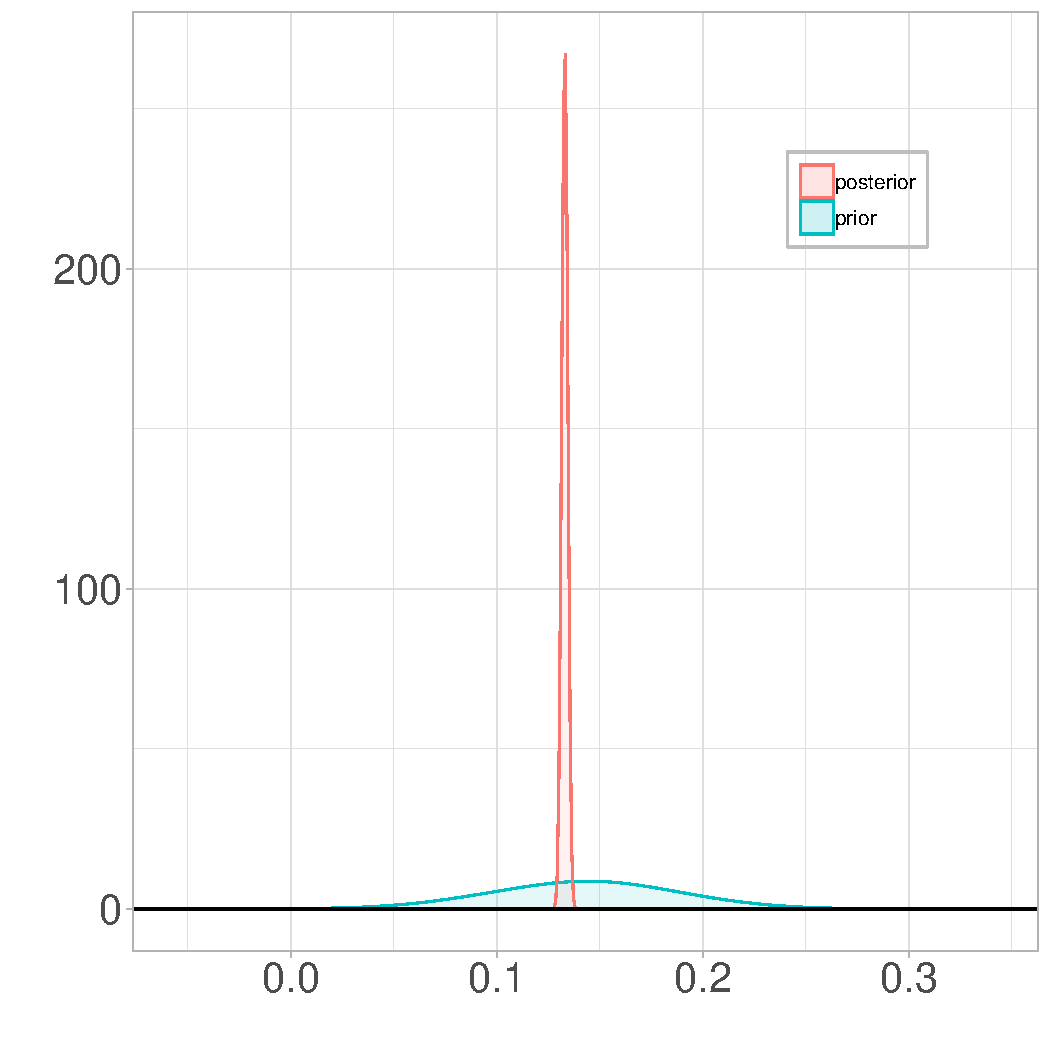
\includegraphics[width=.2\textwidth]{new/Model1/eta.pdf}
    &  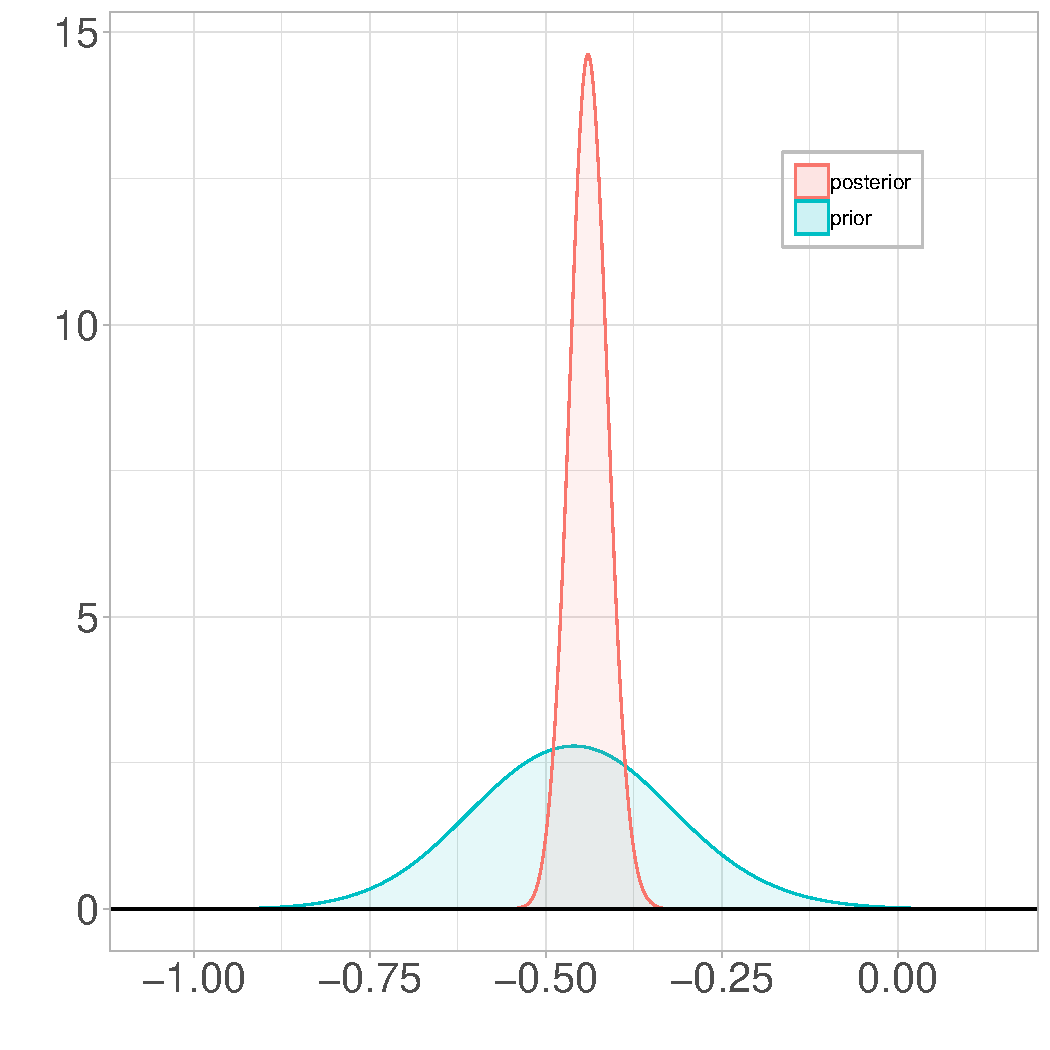
\includegraphics[width=.2\textwidth]{new/Model1/mu.pdf}
	&  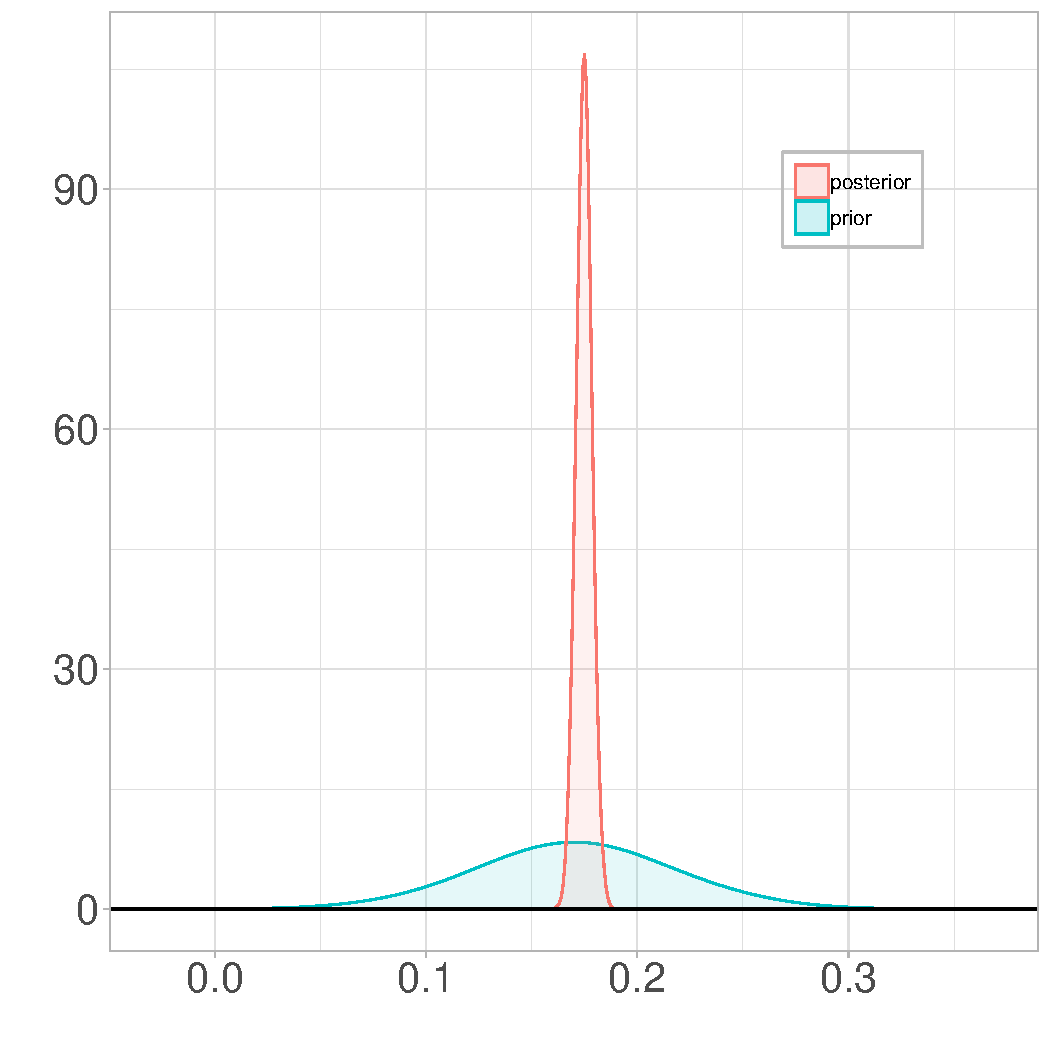
\includegraphics[width=.2\textwidth]{new/Model1/ar.pdf}
	&  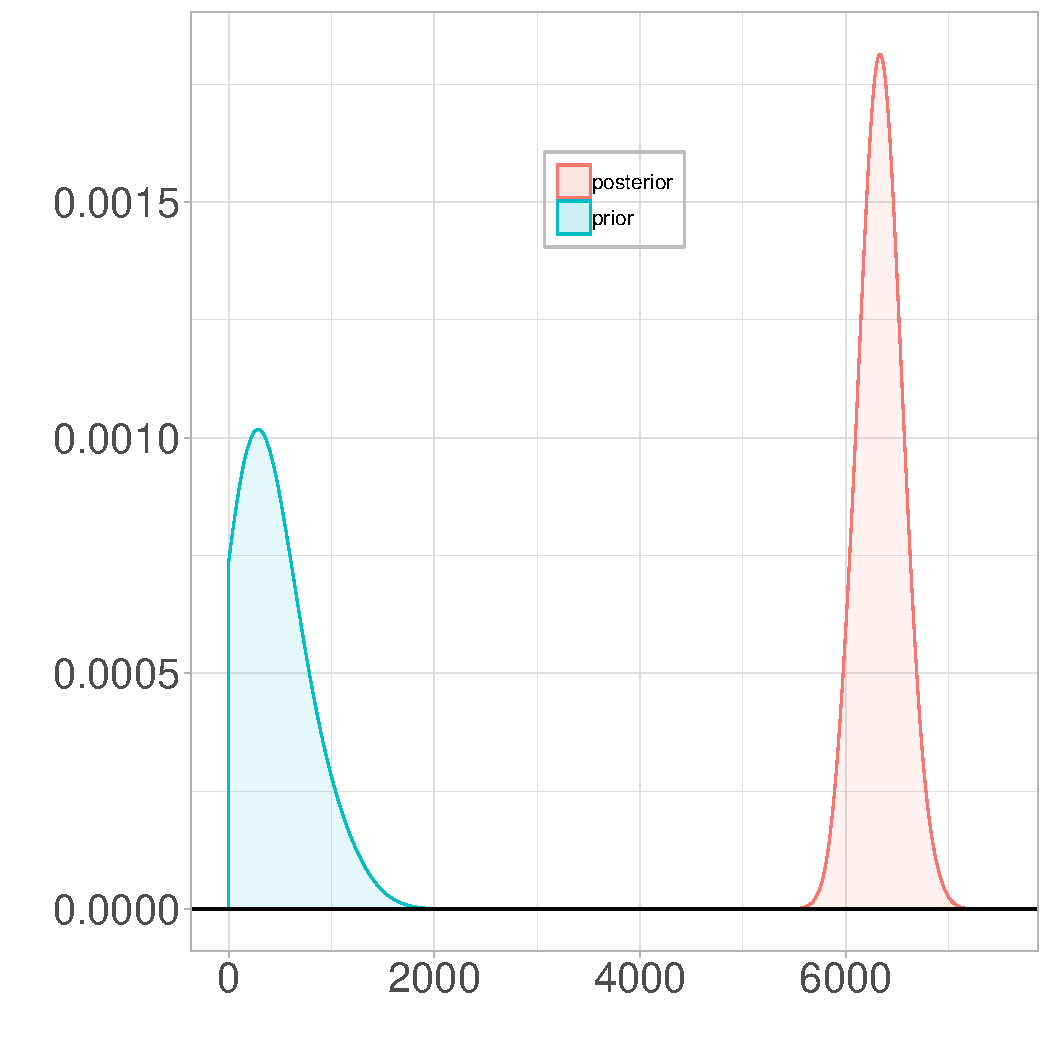
\includegraphics[width=.2\textwidth]{new/Model1/Serr.pdf}\\
		 & $\eta$ & $\mu_t$ & $a_r$ & $\sigma_{err}^2$\\
	&&&&\\
    \rotatebox{90}{ \hspace{3em} \footnotesize $\mathcal{M}_2$}
    & 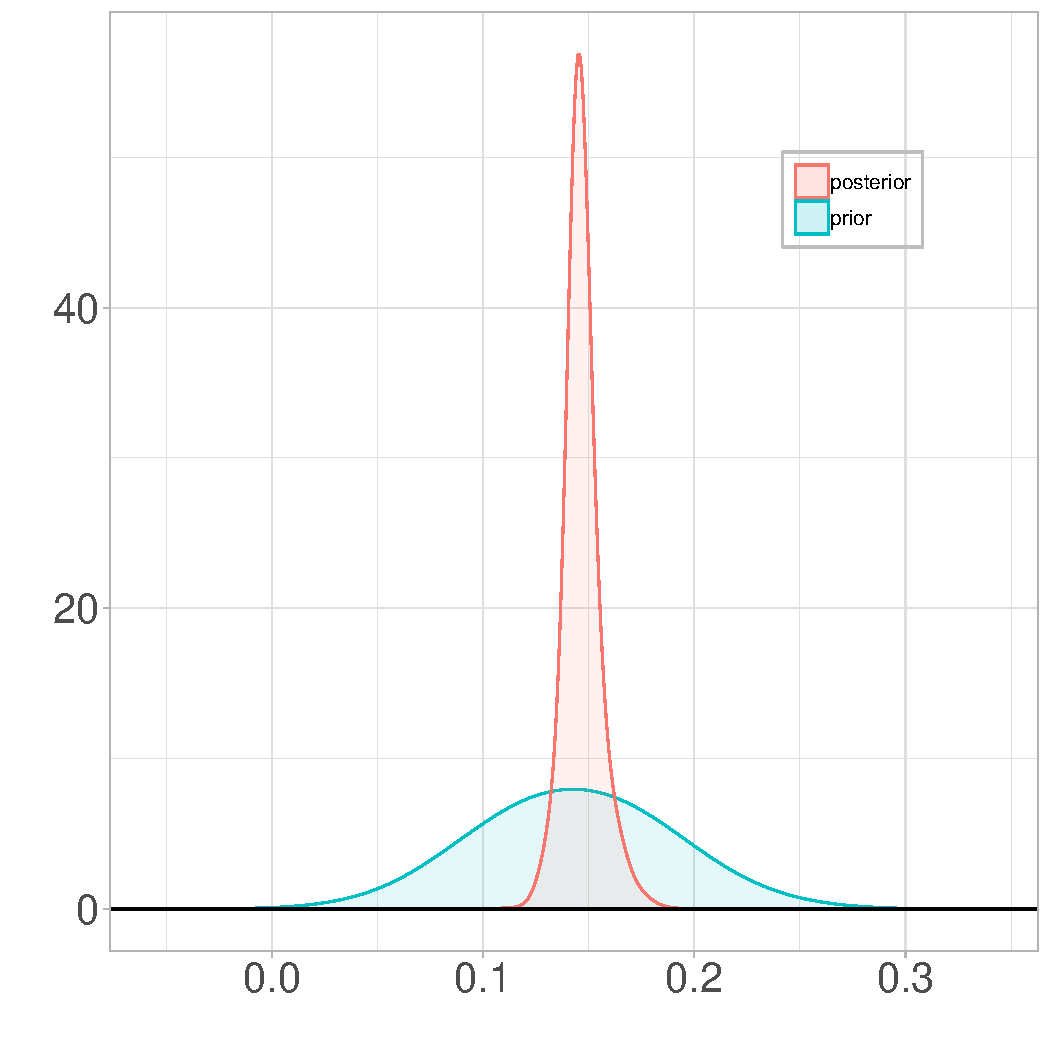
\includegraphics[width=.2\textwidth]{new/Model2/eta.pdf}
    &  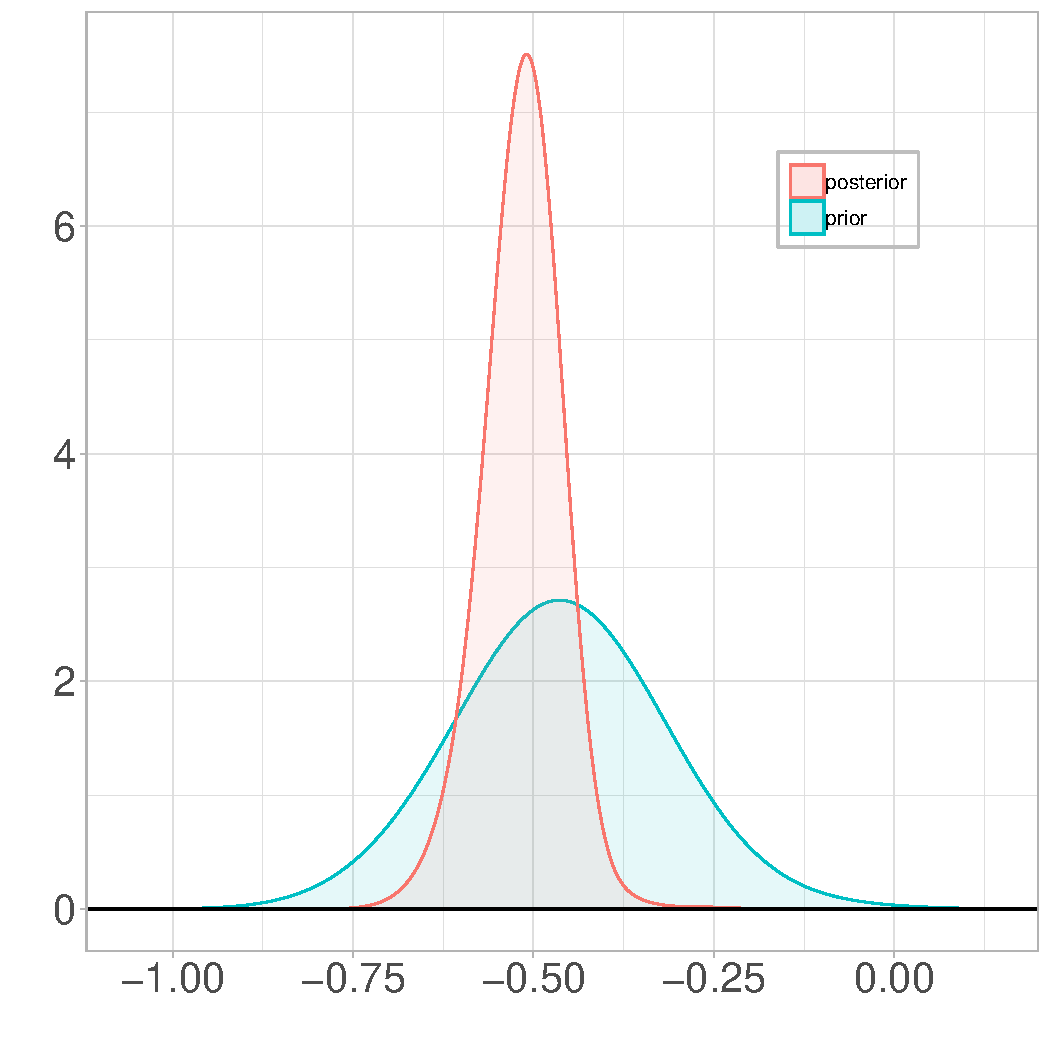
\includegraphics[width=.2\textwidth]{new/Model2/mu.pdf}
	&  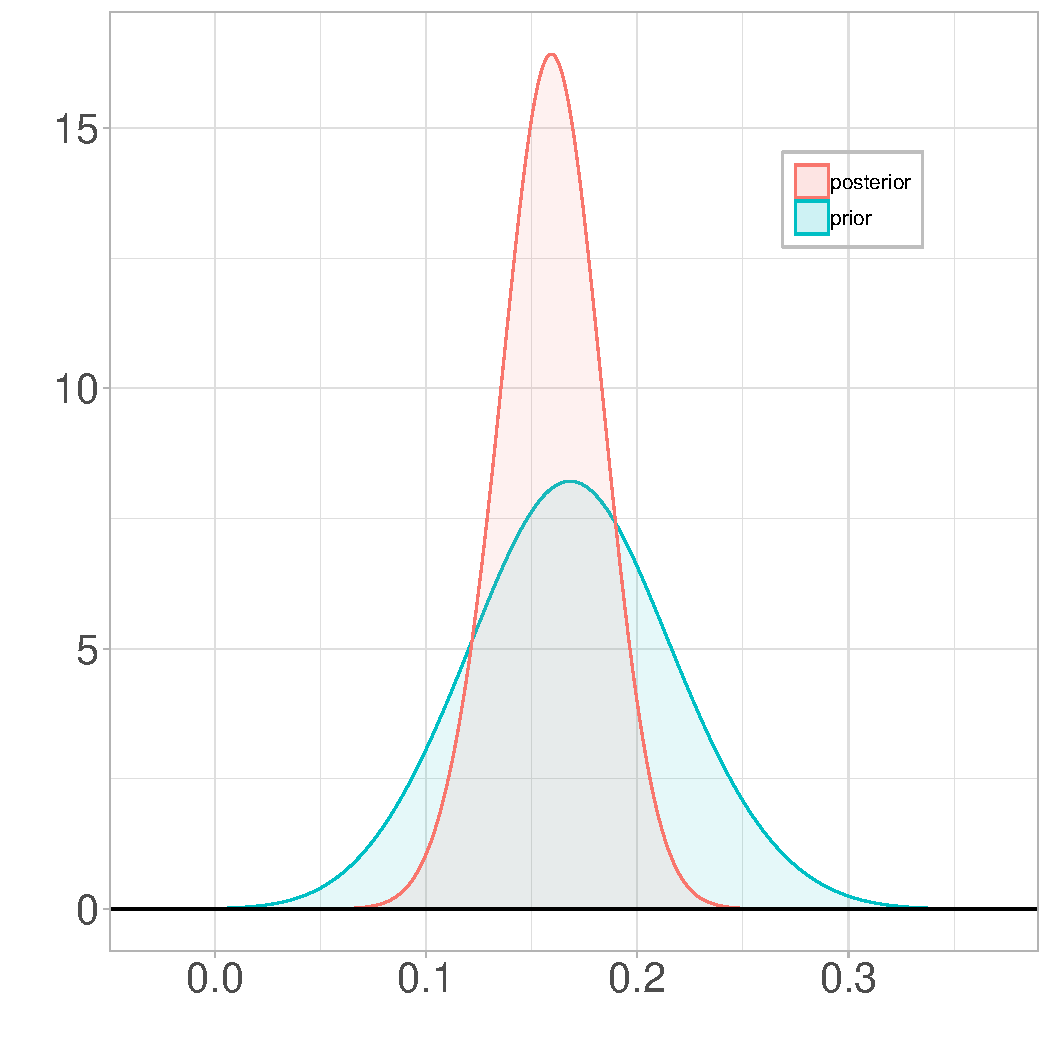
\includegraphics[width=.2\textwidth]{new/Model2/ar.pdf}
	&  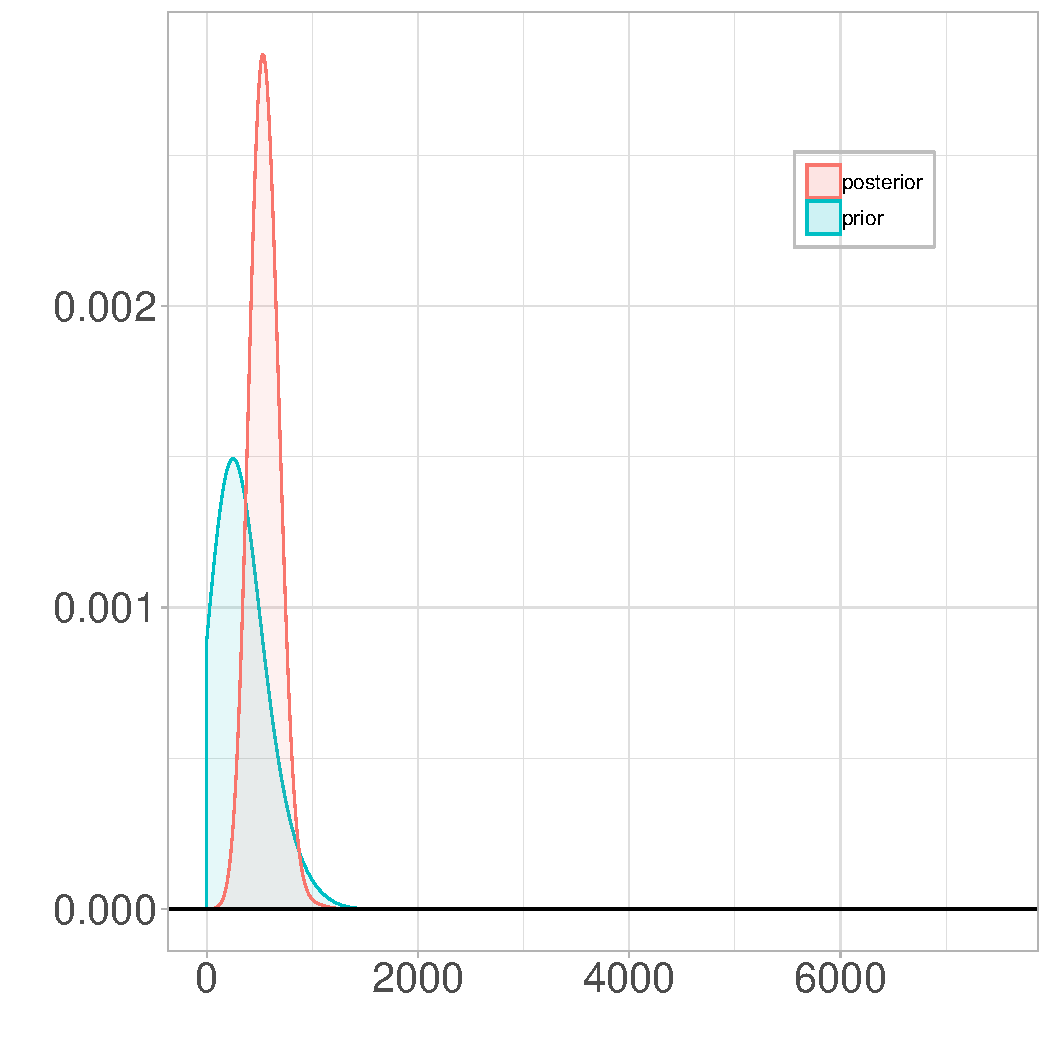
\includegraphics[width=.2\textwidth]{new/Model2/Serr.pdf}\\
		 & $\eta$ & $\mu_t$ & $a_r$ & $\sigma_{err}^2$\\
	&&&&\\
    \rotatebox{90}{ \hspace{3em} \footnotesize $\mathcal{M}_3$}
    & 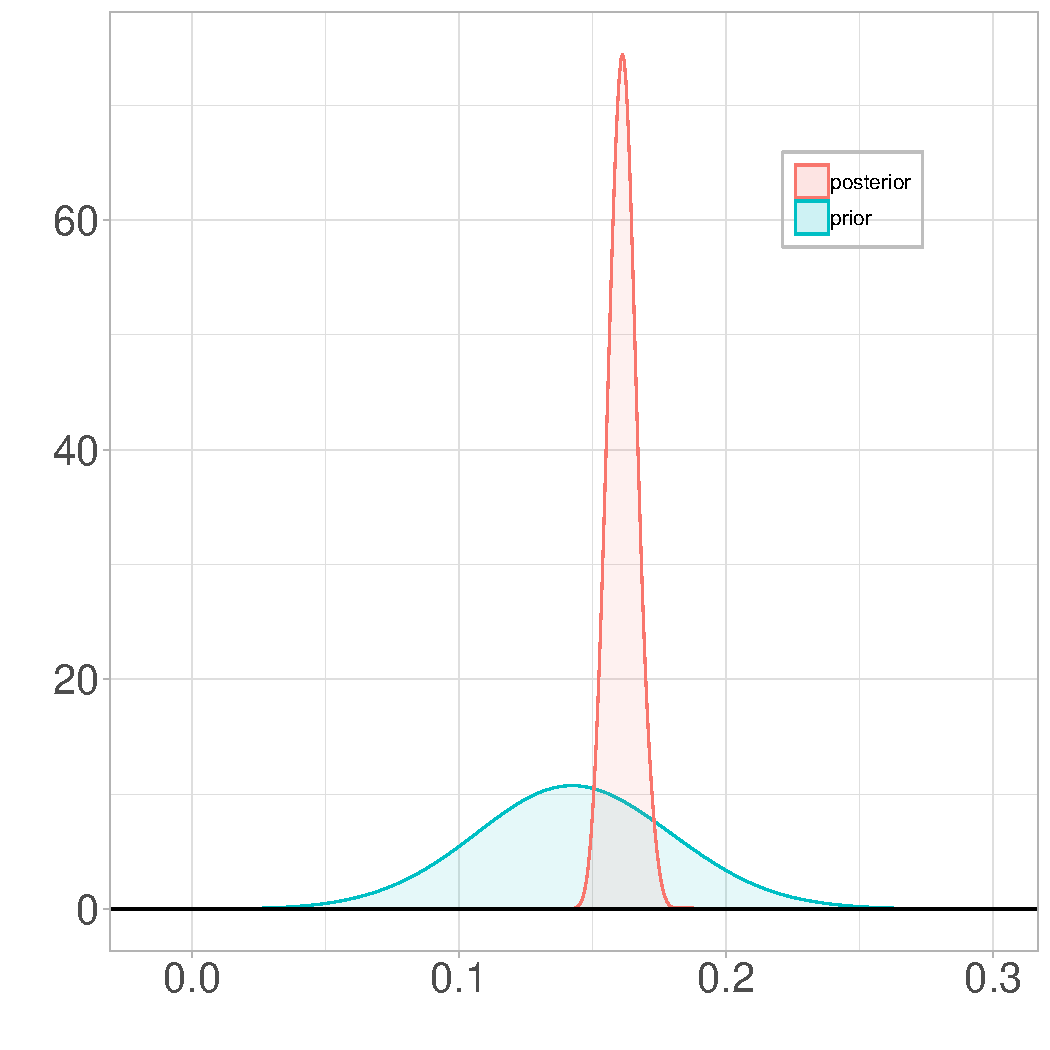
\includegraphics[width=.2\textwidth]{new/Model3/eta.pdf} 
    &  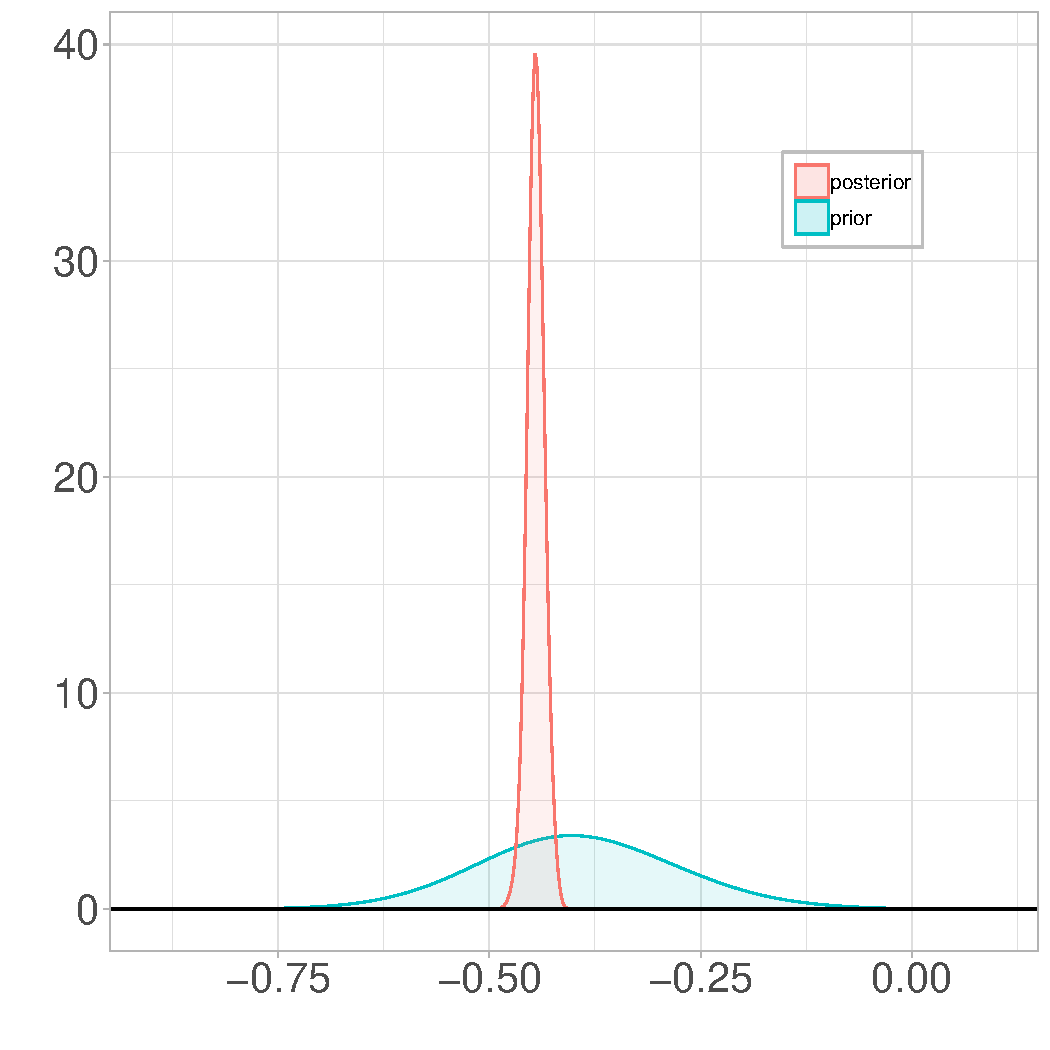
\includegraphics[width=.2\textwidth]{new/Model3/mu.pdf}
	&  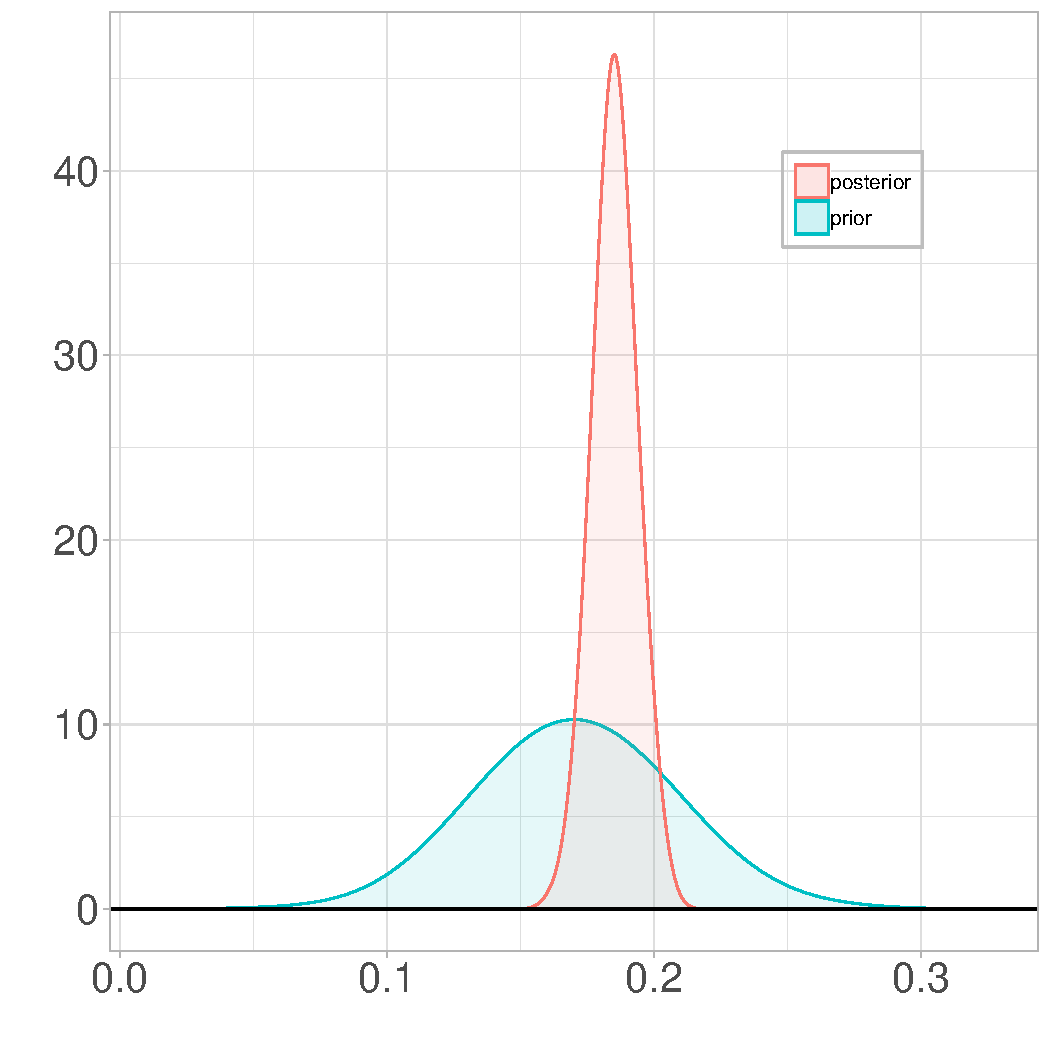
\includegraphics[width=.2\textwidth]{new/Model3/ar.pdf}
	&  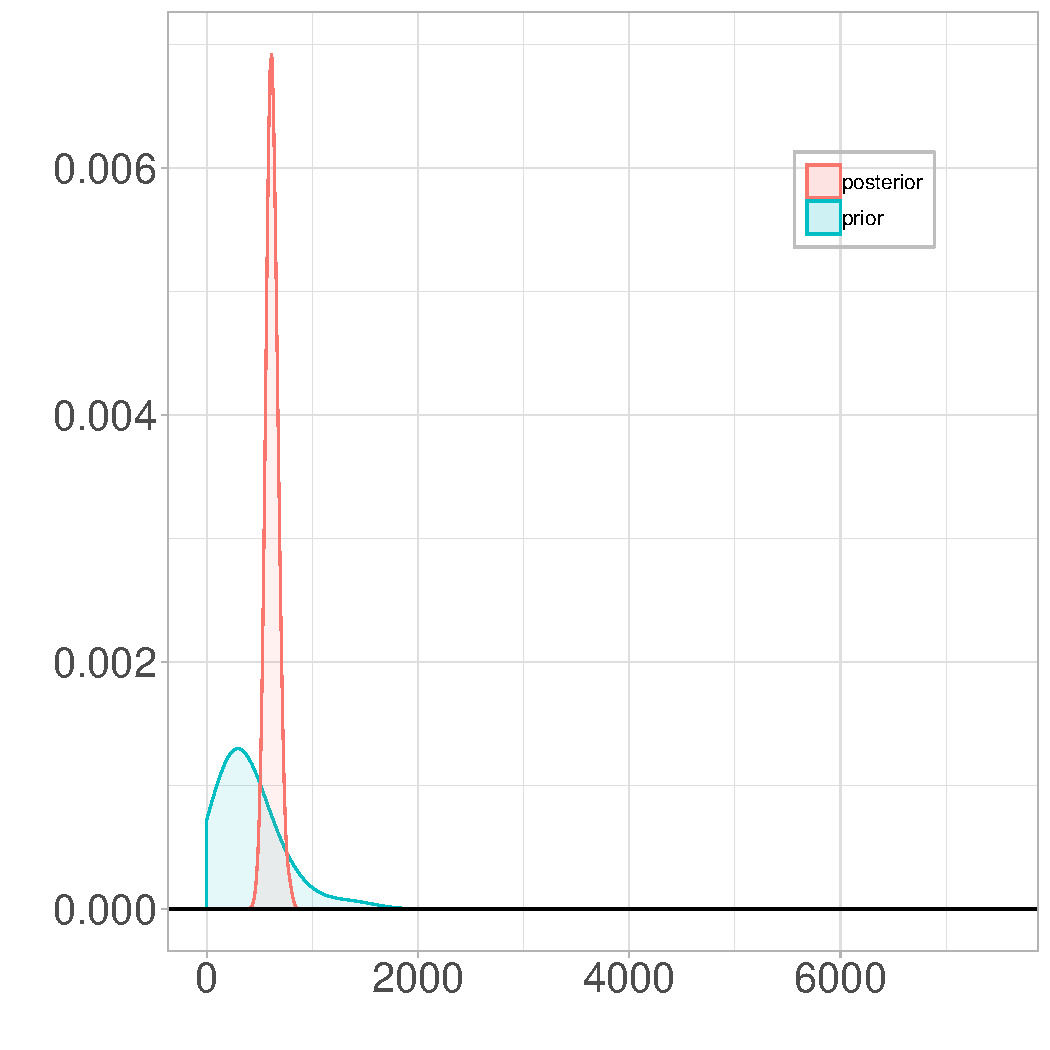
\includegraphics[width=.2\textwidth]{new/Model3/Serr.pdf}\\
		 & $\eta$ & $\mu_t$ & $a_r$ & $\sigma_{err}^2$\\
	&&&&\\
    \rotatebox{90}{ \hspace{3em} \footnotesize $\mathcal{M}_4$}
    & 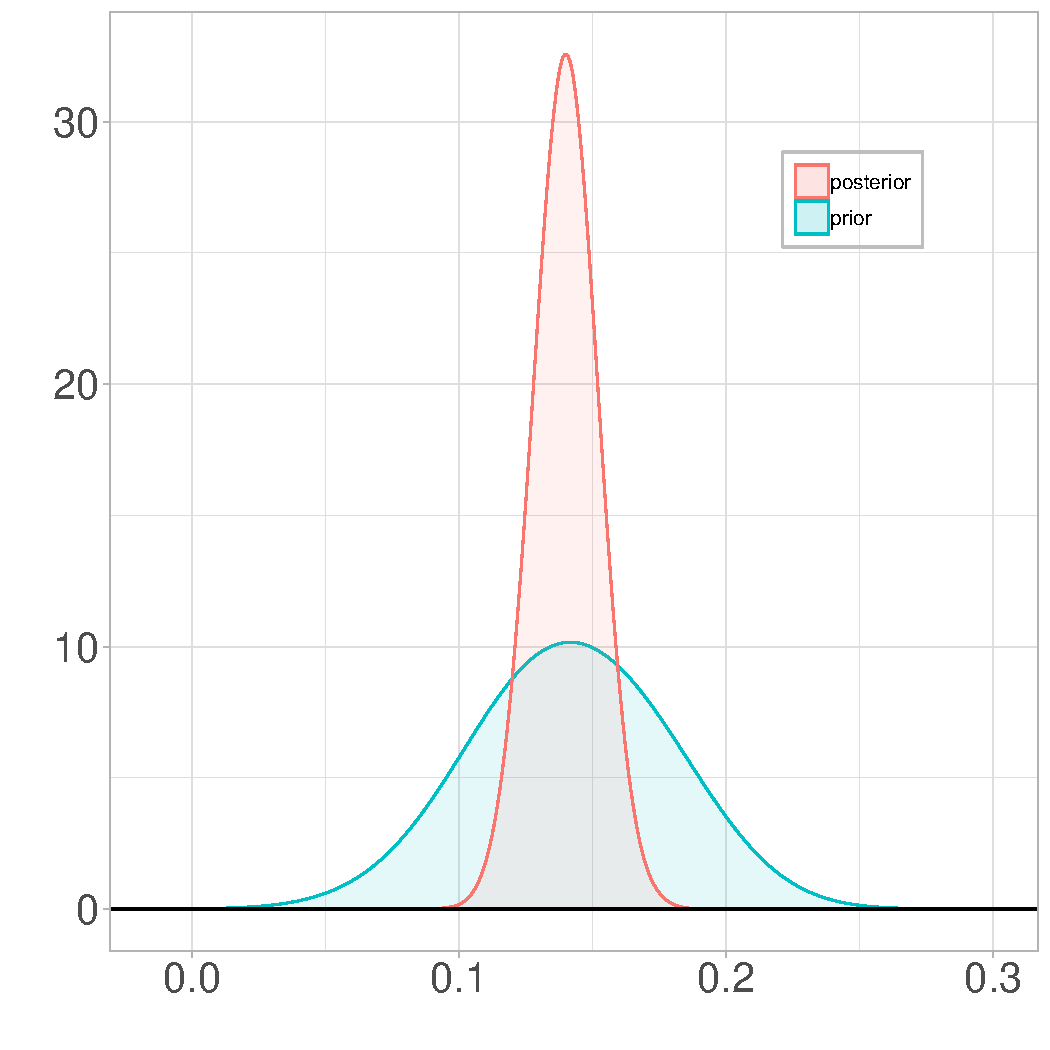
\includegraphics[width=.2\textwidth]{new/Model4/eta.pdf} 
    &  \includegraphics[width=.2\textwidth]{new/Model4/mu.pdf}
	&  \includegraphics[width=.2\textwidth]{new/Model4/ar.pdf}
	&  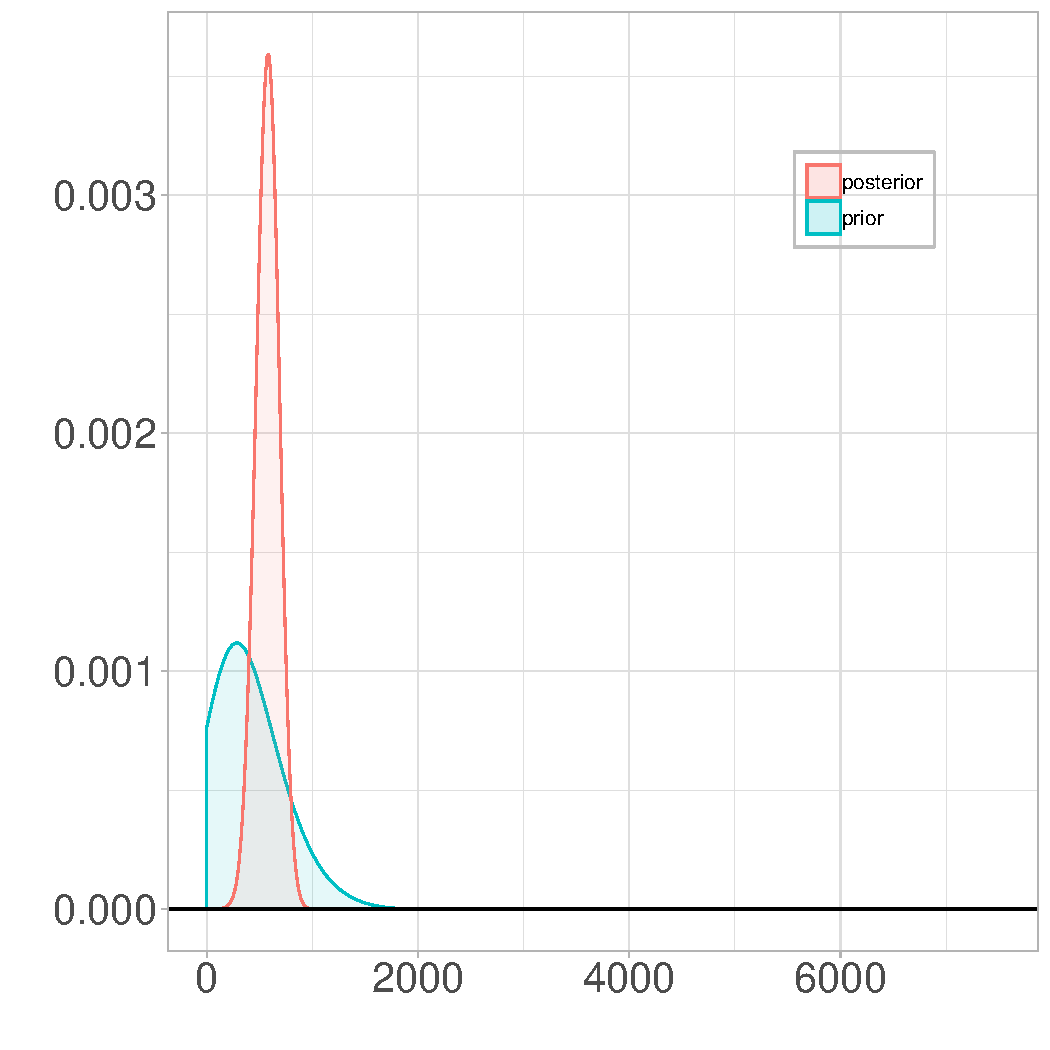
\includegraphics[width=.2\textwidth]{new/Model4/Serr.pdf}\\
	 & $\eta$ & $\mu_t$ & $a_r$ & $\sigma_{err}^2$\\
  \end{tabular}
\caption{\textit{Prior} (in blue) and posterior (in red) densities of $\eta$, $\mu_t$, $a_r$ and $\sigma_{err}^2$ for each model.
On the two first column the two first models (without and with surrogate) which have only these four parameters to estimate.
The two other columns represent the third and the fourth models which have two more parameters to estimate (see Figure \ref{fig:comparisionDensities2}).}
\label{fig:comparisionDensities1}
\end{center}
\end{figure}

\newpage




\begin{figure}[htbp!]
\begin{center}
  \begin{tabular}{ccccc}
    \rotatebox{90}{ \hspace{3em} \footnotesize $\mathcal{M}_2'$}
    & 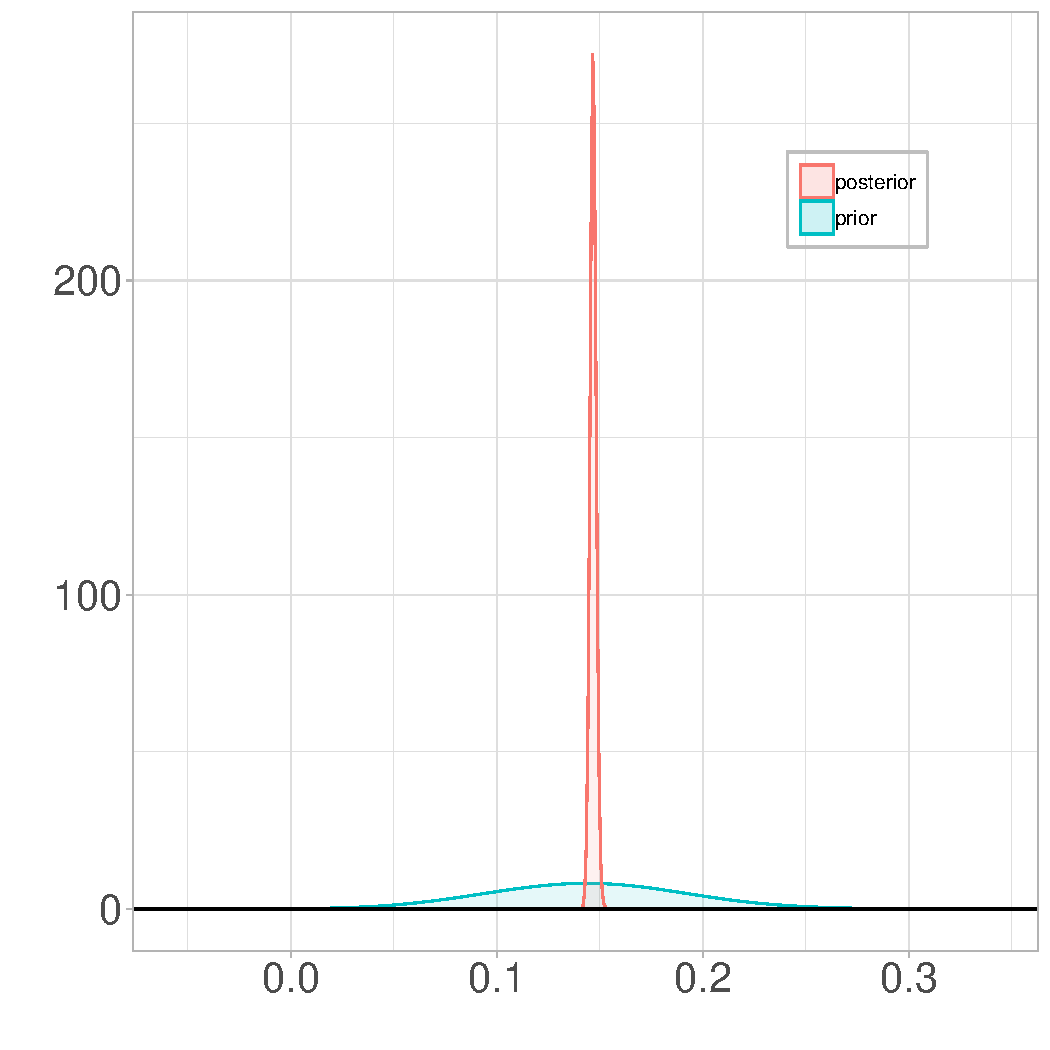
\includegraphics[width=.2\textwidth]{new/Model2sd/eta.pdf}
    & 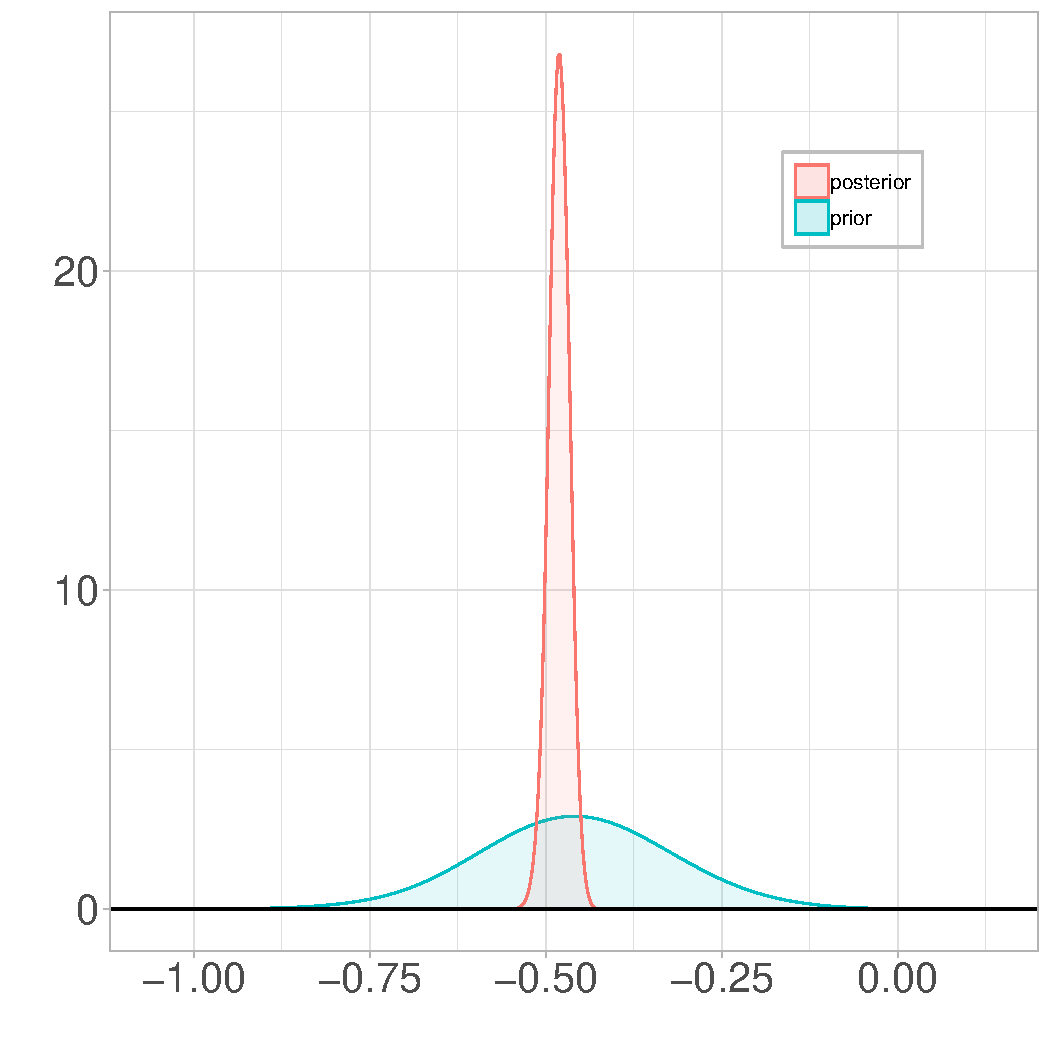
\includegraphics[width=.2\textwidth]{new/Model2sd/mu.pdf}
    & 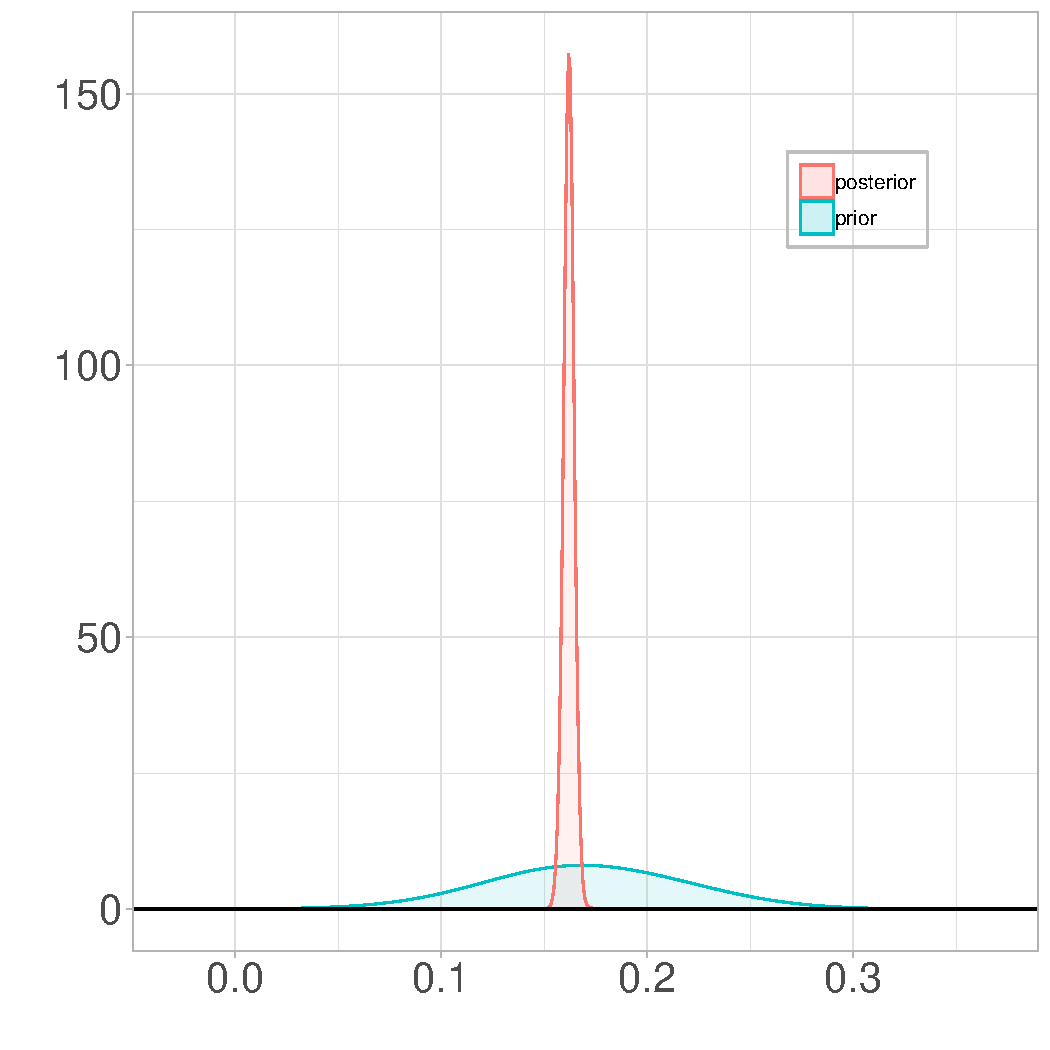
\includegraphics[width=.2\textwidth]{new/Model2sd/ar.pdf}
    & 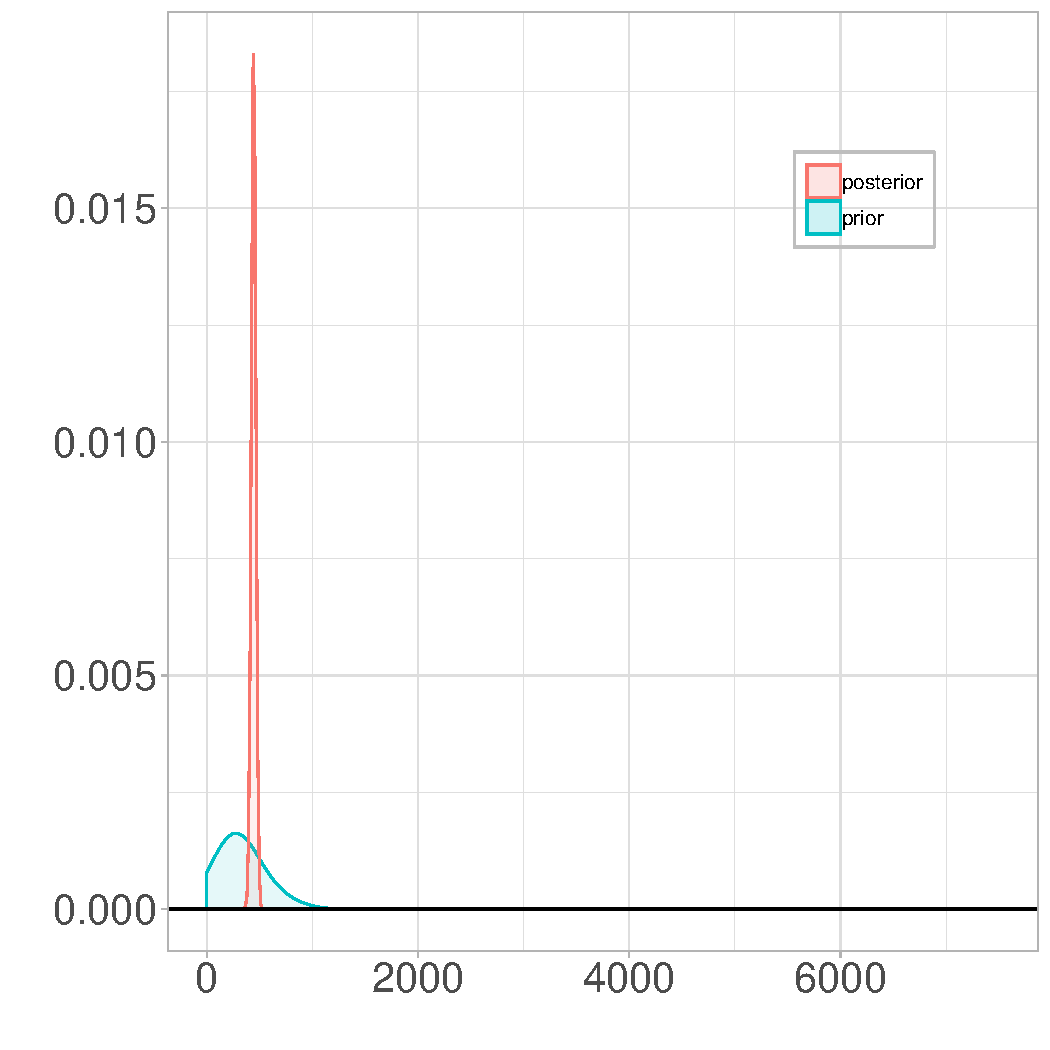
\includegraphics[width=.2\textwidth]{new/Model2sd/Serr.pdf}\\
	& $\eta$ & $\mu_t$ & $a_r$ & $\sigma_{err}^2$\\
	&&&&\\
    \rotatebox{90}{ \hspace{3em} \footnotesize $\mathcal{M}_4'$}
    &  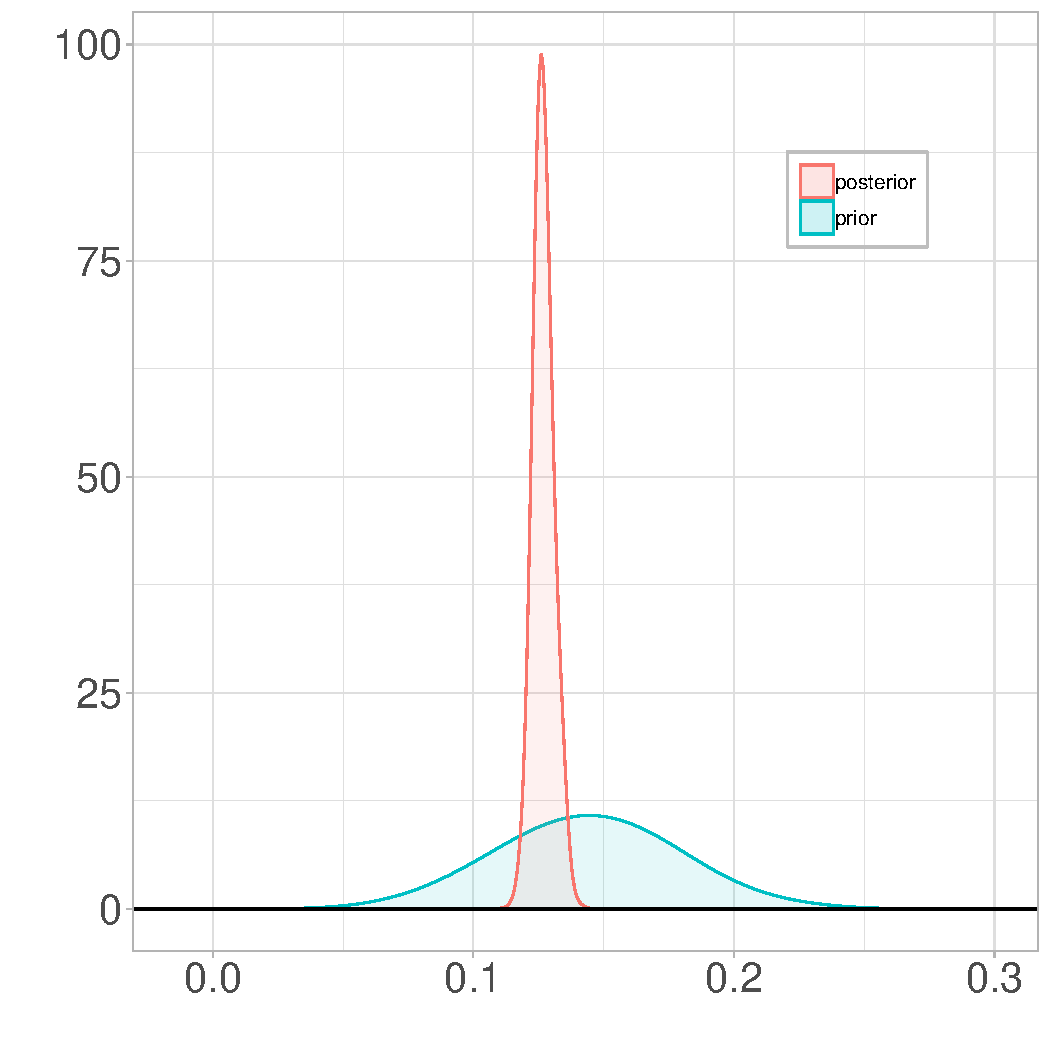
\includegraphics[width=.2\textwidth]{new/Model4sd/eta.pdf}
    &  \includegraphics[width=.2\textwidth]{new/Model4sd/mu.pdf}
    &  \includegraphics[width=.2\textwidth]{new/Model4sd/ar.pdf}
	&  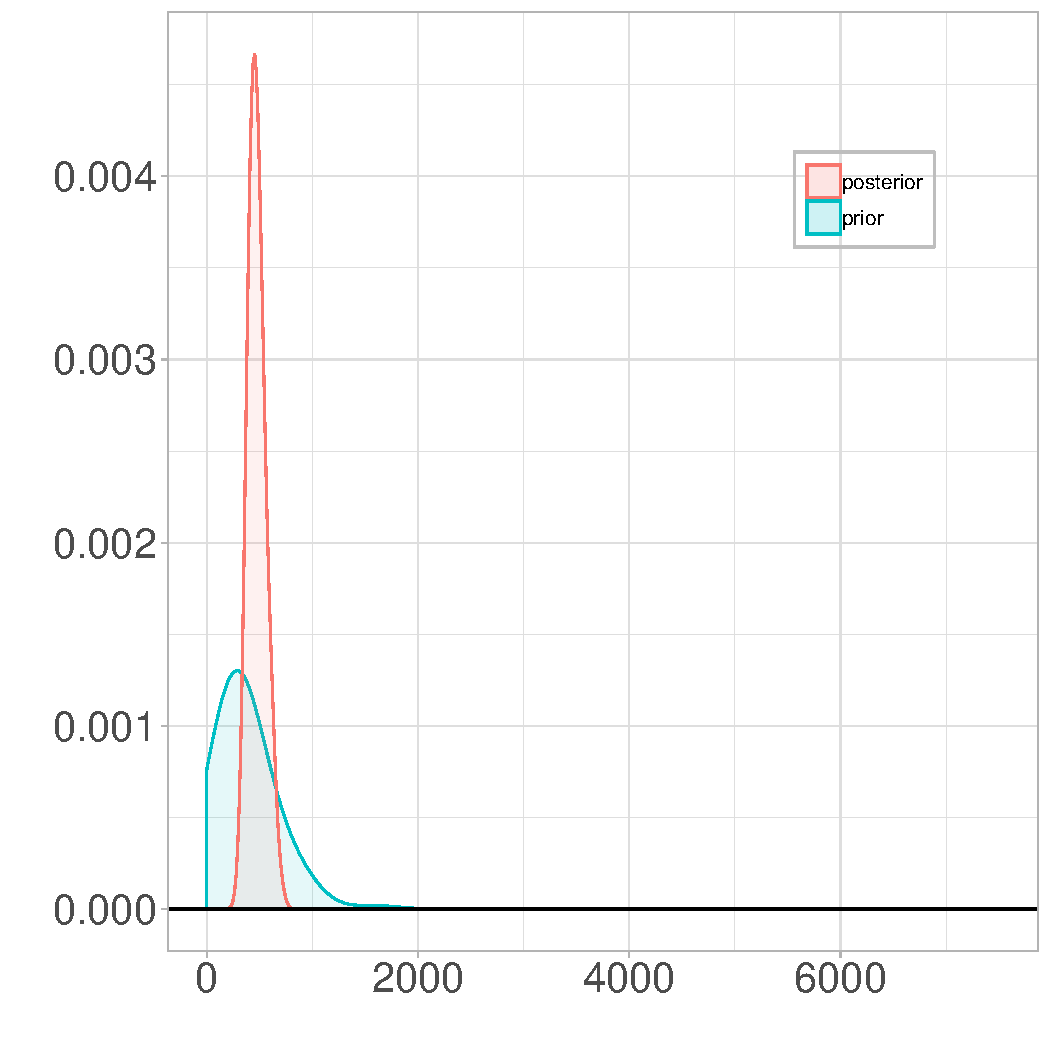
\includegraphics[width=.2\textwidth]{new/Model4sd/Serr.pdf}\\
		 & $\eta$ & $\mu_t$ & $a_r$ & $\sigma_{err}^2$\\
	&&&&\\
  \end{tabular}
\caption{Calibration results for $\mathcal{M}_2'$ and $\mathcal{M}_4'$ which uses the surrogate based on the sequential design.}
\label{fig:calibrationSeq}
\end{center}
\end{figure}



%\newpage

 %We can also notice that, for $\mathcal{M}_2$, the MAP estimator value seems coherent with the physical model. The surrogate used as a replacement of the code have introduced more uncertainties and, trying to compensate the bias introduced, calibration have found parameters densities which match more the reality with the surrogate.\newline

% However, the estimation of $\boldsymbol{\theta}$ is different from those obtained with the first model.
 
The results of calibration performed for each model is displayed in Figure \ref{fig:calibrationSeq}. For each model, the \textit{prior} and the \textit{posterior} densities are confronted and in each case, it illustrates that a decrease of the variance which shows that calibration had improved the \textit{prior} knowledge. However the decrease of variance is not equal for every model. Indeed, in $\mathcal{M}_1$ the variances \textit{a posteriori} are lower than for $\mathcal{M}_2$. When the code is replaced by a surrogate based on a DOE of $50$ points, a term of variance is added (see equation (\ref{eq:VarianceFullLikelihood})) and the estimation is less accurate. The same phenomenon appears when comparing $\mathcal{M}_1$ and $\mathcal{M}_3$. The add of the discrepancy has brought a new term in the variance in the likelihood which increase the variance \textit{a posteriori}. The model $\mathcal{M}_4$ which combines a surrogate and a discrepancy has then a bigger variance \textit{a posteriori} than with the other models. The right column in Figure \ref{fig:comparisionDensities1} illustrates the \textit{prior} and \textit{posterior} of the variance of the white Gaussian noise. A strong disagreement appears in the model $\mathcal{M}_1$ because the \textit{posterior} mode of $\sigma_{err}^2$.

 
%From $\mathcal{M}_1$ to $\mathcal{M}_2$, a surrogate emulates the numerical code. Figure \ref{fig:comparisionDensities1} illustrates
%a bigger variance \textit{a posteriori} for the parameters densities of $\mathcal{M}_2$ than $\mathcal{M}_1$. Replacing the code by
%a surrogate, a low number of points, had brought more uncertainty.


% Moreover, the densities for $\mathcal{M}_2$ appear to be out of step with $\mathcal{M}_1$.
%Calibration behaves as if a bias has appeared with the surrogate. 
%This is worth to note that using a surrogate not only increase the variance of the posterior distribution of the parameter $\boldsymbol{\theta}$ but may also have an impact on the mode. This is also observed when moving from $\mathcal{M}_3$ to $\mathcal{M}_4$. 
%%This looks coherent with the results given Table \ref{tab:comparisonPG}, because the chosen surrogate with a small number of points is not a fairly good representation of the code.
%Calibration seems to be less accurate when one uses a surrogate instead of the code. Degrading calibration just by using a surrogate 
% Calibration is, then, altered by the surrogate which does not represent well enough the numerical code. When one possesses a time consuming code, one must be careful to the quality of the surrogate. It depends mainly on the points chosen in the DOE and some adaptive design have been proposed in literature as \citet{damblin2018} for example. To compare a case where the surrogate would be better, we will consider an initial DOE of $150$ points and we will increase this initial DOE with $10$ points chose according to the algorithm in \citet{damblin2018}. The results are given Figure \ref{fig:calibrationSeq} and illustrate that the \textit{posterior} modes have become consistent with the ones for the models $\mathcal{M}_1$ and $\mathcal{M}_3$.
%Adding the discrepancy (from $\mathcal{M}_1$ to $\mathcal{M}_3$ and from $\mathcal{M}_2$ to $\mathcal{M}_4$) has almost always reduced the variances of the posterior distributions.
%\newline

We also depict correlation between the parameters. As a matter of fact, a strong positive and linear correlation links every parameters ($\eta$, $\mu_t$ and $a_r$) with each other as illustrated Figure \ref{fig:corrPlot}. A strong correlation appears between $\mu_t$ and $a_r$. A lower, but still meaningful, correlation is also visible between $\eta$ and $\mu_r$, and $a_r$ and $\eta$.\newline


\begin{figure}[htbp!]
\begin{center}
  \begin{tabular}{cccccc}
    \rotatebox{90}{ \hspace{4em} \footnotesize $\mu_t$}
    & 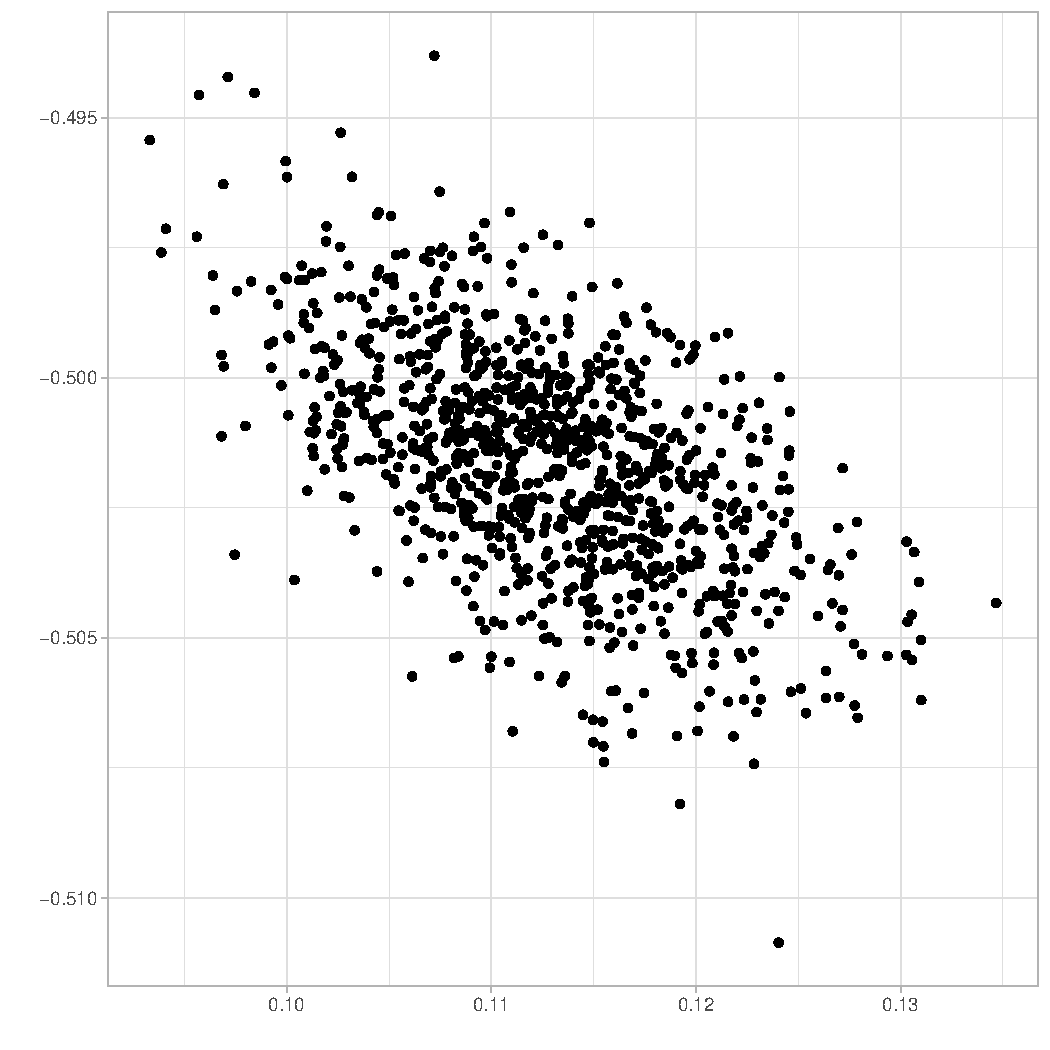
\includegraphics[width=.2\textwidth]{figR/corr12.pdf} 
    &\rotatebox{90}{ \hspace{4em} \footnotesize $a_r$}
    &  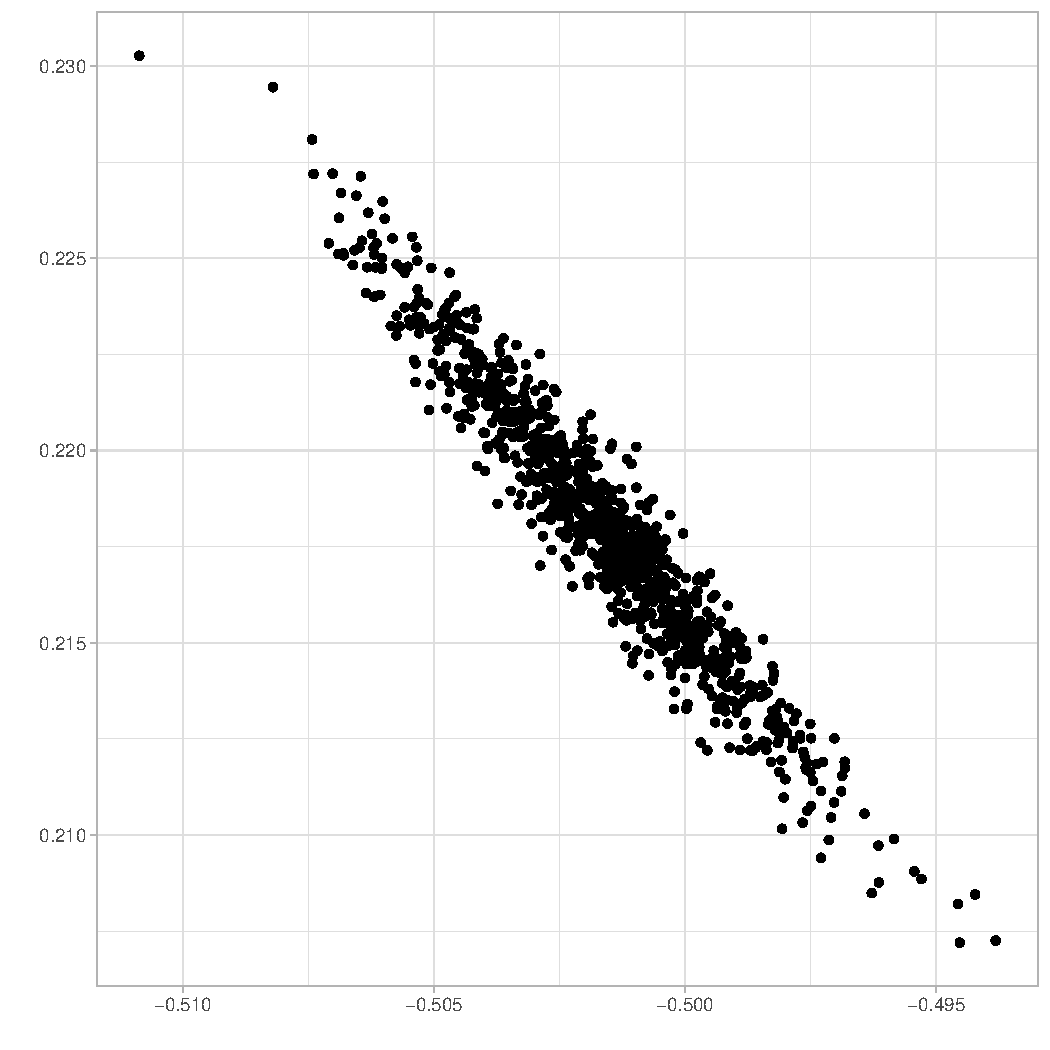
\includegraphics[width=.2\textwidth]{figR/corr23.pdf}
    &\rotatebox{90}{ \hspace{4em} \footnotesize $\eta$}
	&  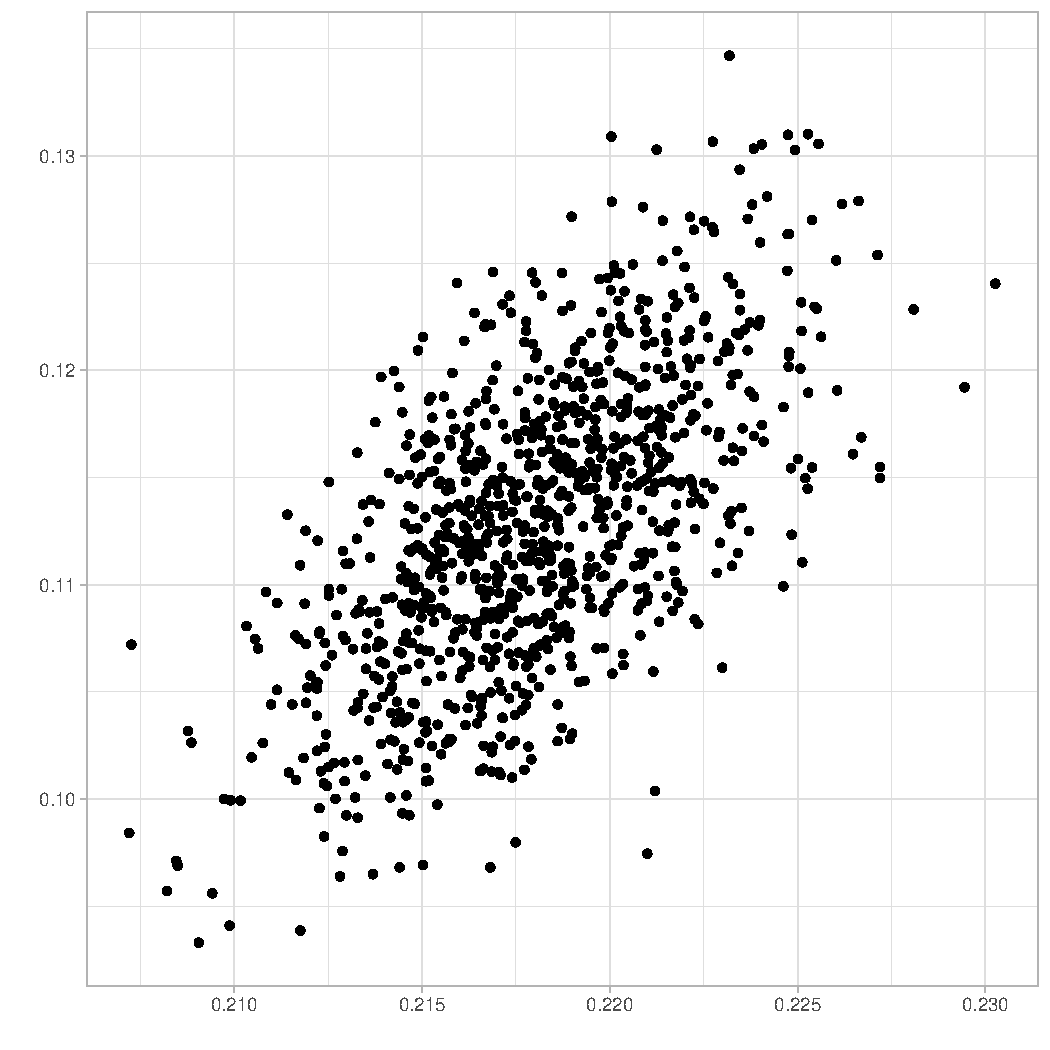
\includegraphics[width=.2\textwidth]{figR/corr31.pdf}
\\
	&$\eta$ & &$\mu_t$ & & $a_r$\\
  \end{tabular}
\caption{Correlation representation between the parameters}
\label{fig:corrPlot}
\end{center}
\end{figure}

%
%\begin{figure}[htbp!]
%\centering
%    \begin{tikzpicture}
%		\tikzstyle{m1}=[]
%		\node[m1] (N1) at (0,0) {\includegraphics[width=.3\textwidth]{figR/corrPlot.pdf}};
%		\node[m1] (N2) at (-2,1) {$\eta$};
%		\node[m1] (N3) at (-1,2) {$\eta$};
%		\node[m1] (N4) at (0,2) {$\mu_t$};
%		\node[m1] (N5) at (-1,0) {$\mu_t$};
%		\node[m1] (N6) at (1,2) {$a_r$};
%		\node[m1] (N6) at (0,-1) {$a_r$};
%    \end{tikzpicture}
%    
%\caption{Correlation representation between the parameters}
%\label{fig:corrPlot}
%\end{figure}

%This disagreement becomes even more important with the second model in which the variance of the \textit{posterior} density is too high to make sense for doing any parameter estimation. However in the third and fourth model, the disagreement has vanished. The maximum \textit{a posteriori} of the measurement error variance even seems to be the coherent regarding \textit{prior} densities.\newline
%  
%In the two first models, the measurement errors are much bigger than expected \textit{a priori}. As a matter of fact, a code error is included and estimated in the $\epsilon's$ without knowing it. Figure \ref{fig:comparisionDensities1} illustrates this phenomenon because, when the discrepancy is modeled, the whole model gets more physical sense. In the two first cases, the maximum \textit{a posteriori} of $\sigma_{err}^2$ is about respectively $1000$ and $6000$. That makes a standard deviation of about $31.62W$ and $77.45W$. Such a measurement error does not physically makes sense.\newline

\begin{figure}[htbp!]
\begin{center}
  \begin{tabular}{cccc}
&  $\mathcal{M}_3$ & $\mathcal{M}_4$ & $\mathcal{M}_4'$ \\
    \rotatebox{90}{ \hspace{3em} \small density}
	&  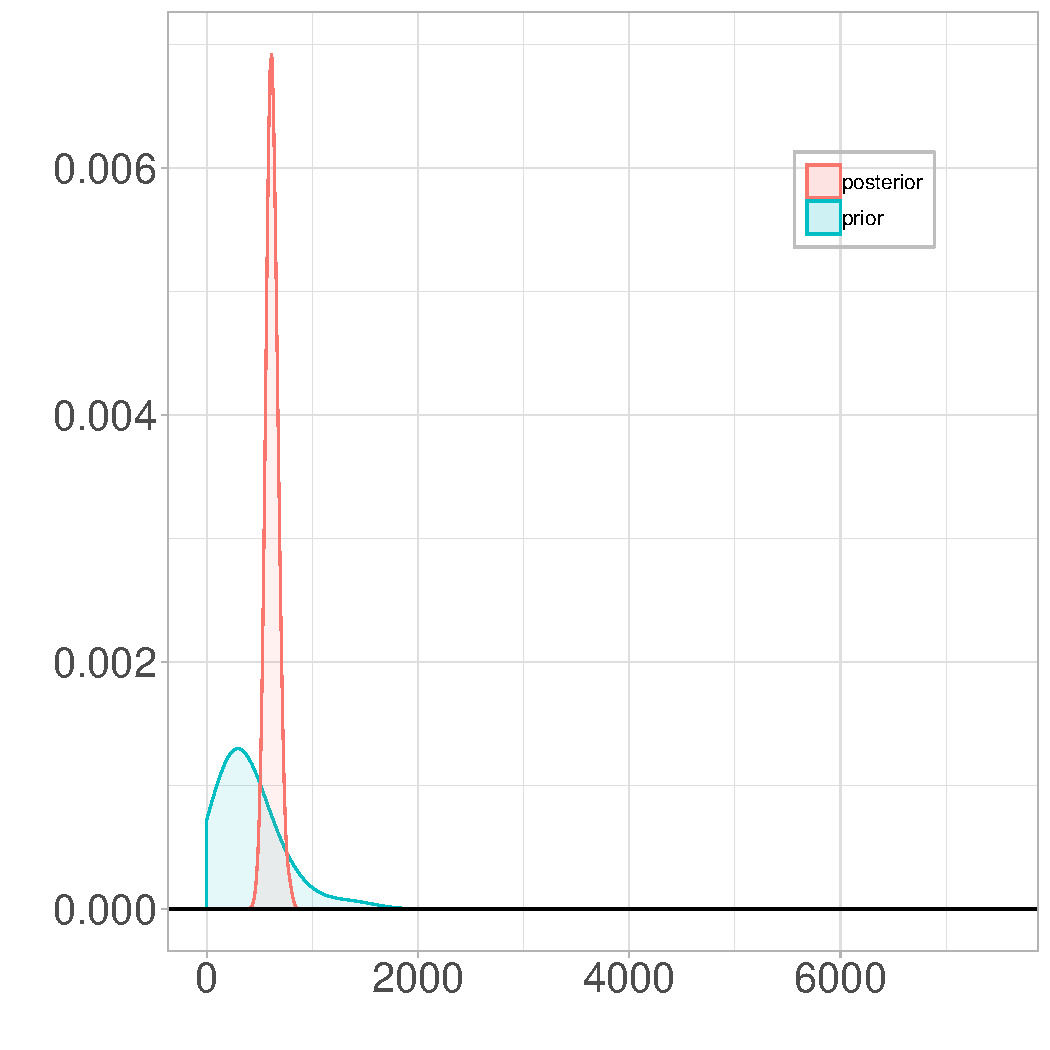
\includegraphics[width=.2\textwidth]{new/Model3/Serr.pdf}
	&  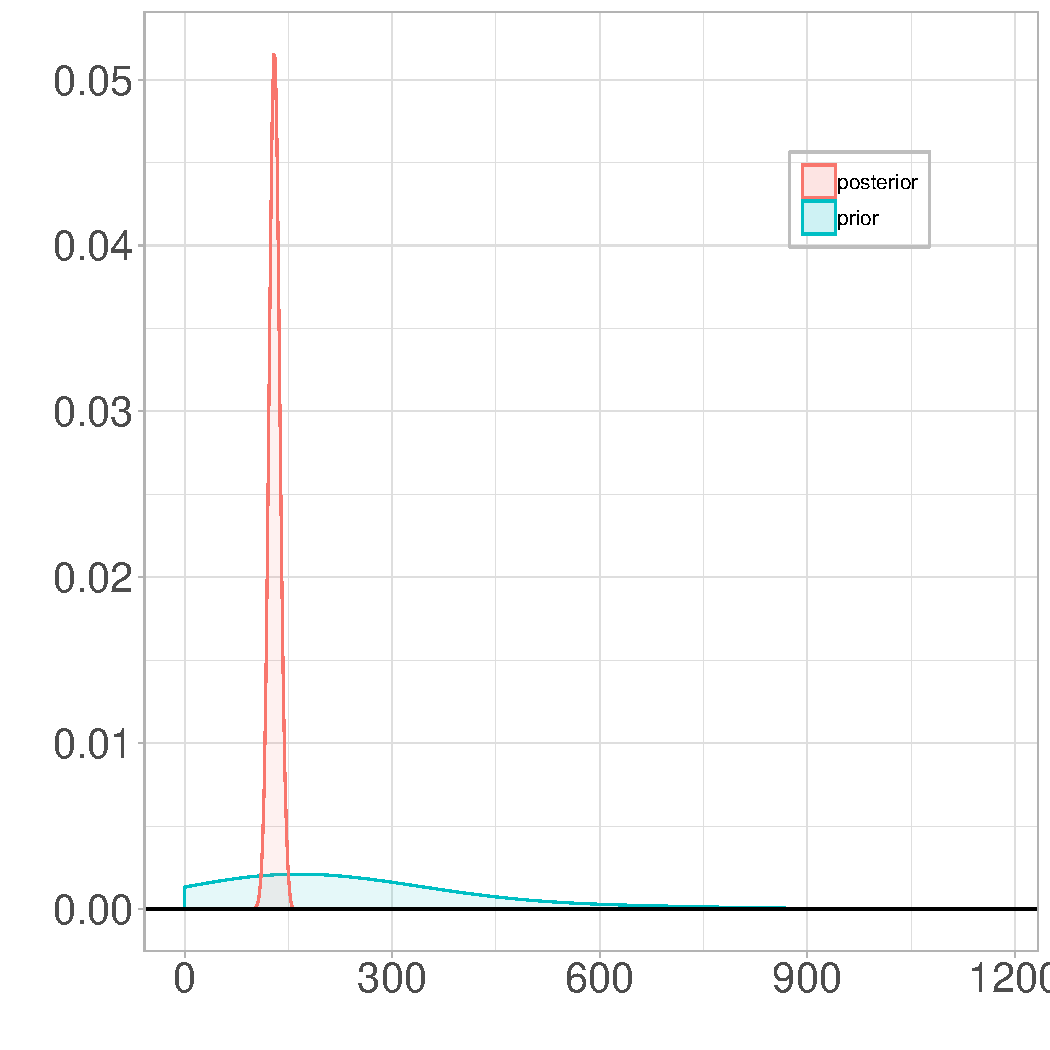
\includegraphics[width=.2\textwidth]{new/Model4/Sig.pdf}
	&  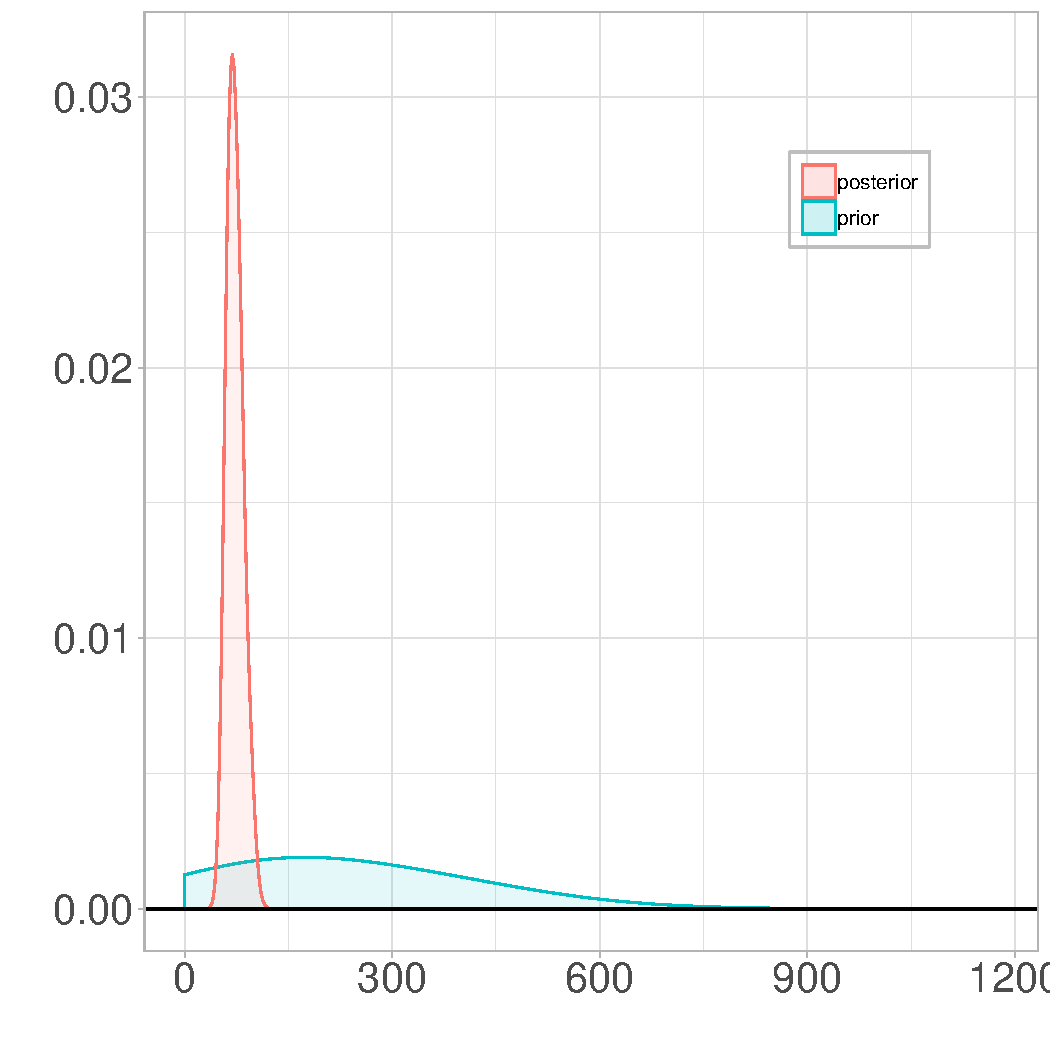
\includegraphics[width=.2\textwidth]{new/Model4sd/Sig.pdf}\\
	&\multicolumn{3}{c}{$\sigma_{\boldsymbol{\delta}}^2$}\\
	&&&\\
    \rotatebox{90}{ \hspace{3em} \small density}
	&  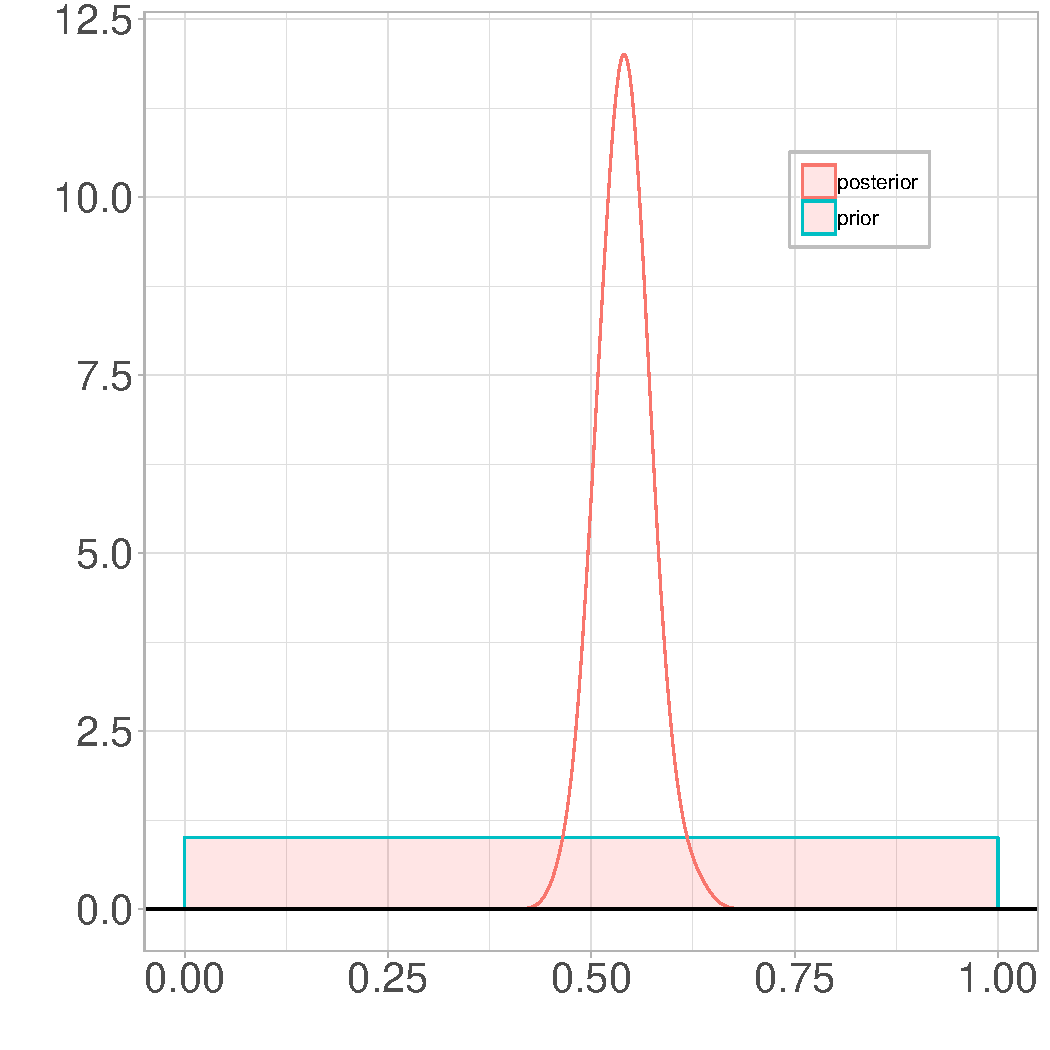
\includegraphics[width=.2\textwidth]{new/Model3/psi.pdf}
	&  \includegraphics[width=.2\textwidth]{new/Model4/psi.pdf}
	&  \includegraphics[width=.2\textwidth]{new/Model4sd/psi.pdf}\\
	&\multicolumn{3}{c}{$\psi_{\boldsymbol{\delta}}$}\\
  \end{tabular}   
\caption{\textit{Prior} (in blue) and posterior (in red) densities of $\sigma_{\boldsymbol{\delta}}^2$ and $\psi_{\boldsymbol{\delta}}$ for $\mathcal{M}_3$, $\mathcal{M}_4$ and $\mathcal{M}_4'$.}
\label{fig:comparisionDensities2}
\end{center}
\end{figure}

Figure \ref{fig:comparisionDensities2} illustrates the estimation of the parameters from the discrepancy term.
As expected, learning from data has improved our \textit{prior} belief by decreasing the \textit{prior} uncertainty of the parameters. 
It shows that in both cases (with and without surrogate) that the convergence seems to be reached at some point. \newline
%The fact that the values may slightly differ from each other is not an issue because the models are intrinsically different. \newpage

\subsection{Comparison}

To compare the prediction ability of the four models,
a cross validation (CV) is performed.
Three days of data (chosen randomly) are taken off the calibration dataset for each of the $100$ repetitions of the CV. 
The power densities, generated from the MCMC samples, allow us to compute, for each model, the $90\%$ predictive credibility intervals. 
The coverage rate at $90\%$ represents the quantity of validation experiments contained in these credibility intervals.
The Root Mean Square Error (RMSE) is also computed for the instantaneous power. The results are displayed Table 
\ref{tab:comparison}.\newline
%A visual check is also done on random MCMC chains to testify the good accuracy of the mixing properties.

\begin{table}[htbp!]
\centering
\caption{Comparison of the RMSEs and coverage rates in prediction of 100 test-sets on three randomly selected days where $\mathcal{M}_2'$ and $\mathcal{M}_4'$ are the models based on the Gaussian process established after the sequential design}
\label{tab:comparison}
\begin{tabular}{c|c|c|c|c|c|c}

& $\mathcal{M}_1$ & $\mathcal{M}_2$ & $\mathcal{M}_3$ & $\mathcal{M}_4$ & $\mathcal{M}_2'$&  $\mathcal{M}_4'$ \\
\hline
\hline
coverage rate at 90\% (in \%) & 91 & 32 & 87 & 23 & 64 & 0 \\
\hline
RMSE of the instantaneous power ($W$) & 5.1 & 21.79 & 10.94 & NANY & 4.56 & NANY \\
\end{tabular}
\end{table}

The coverage rates for $\mathcal{M}_1$ and $\mathcal{M}_3$ corresponds to the chosen credibility level.
However for $\mathcal{M}_2$ and $\mathcal{M}_4$ 
the coverage rates are below this level. As expected the coverage rates of $\mathcal{M}_2'$ and $\mathcal{M}_4'$



This was expected since the coverage rates for the code emulation displayed in Table \ref{tab:comparisonPG} were below the fixed credibility level
especially when the DOE had only $50$ points. We recall that these coverage rates only account for the surrogate error and not for the uncertainty
on $\boldsymbol{\theta}$.
We also notice that the predictive power increases when the discrepancy is added. \newline


%The cover rate seems to be quite good for $\mathcal{M}_1$, $\mathcal{M}_3$ and $\mathcal{M}_4$. However, for $\mathcal{M}_2$, the rate is lower because the Gaussian process which emulates the code had difficulties to reach every points of the outputs of the code (which is due to high fluctuations). The comparison of the RMSE of the instantaneous power leads to a similar conclusion. The different models $\mathcal{M}_1$, $\mathcal{M}_3$ and $\mathcal{M}_4$ reach a good estimation. Even for the integrated energy, the results are similar. It is interesting to note that the discrepancy did improve a little the initial computational code (from $\mathcal{M}_1$ to $\mathcal{M}_3$). When the surrogate only is used, the results are not satisfactory ($\mathcal{M}_2$). However when the discrepancy is added to the surrogate, the prediction is a lot better ($\mathcal{M}_4$).\newline

Overall, the model $\mathcal{M}_3$ has better results than the others. 
This conclusion can be explained twofold. First, the code realizes a better prediction than the surrogate.
Second, a correlation structure remains in the error. Adding the discrepancy in the model allows to catch up the real results.
The fact that the models, encompassing a surrogate, produces worse results is expected. The Gaussian process used for the surrogate had trouble to fill every variation of power. To compensate this lack of information, the posterior credibility interval becomes wide and less informative.\newline


%Overall, the model $\mathcal{M}_4$ has better results than the others. This conclusion can be explained by the fact that the surrogate tries to smooth the response of the code, and each time the surrogate is called, it reproduces an error. The discrepancy trends to counter this error. Very surprisingly, $\mathcal{M}_4$ does a better job than $\mathcal{M}_3$ (although the latter can freely access as many runs of the code as required). This might be explained because the Gaussian process used for simulating the discrepancy has a better matching association with other Gaussian processes. The code encounters a lot of fluctuations and as we can see Table \ref{tab:comparison}, the discrepancy has more trouble to estimate its code error (from $\mathcal{M}_1$ to $\mathcal{M}_3$) than the one from the surrogate (from $\mathcal{M}_1$ to $\mathcal{M}_3$). \newline

%The interest of calibration is to assess, in a better way, the error of a quantity of interest. 
%For example, Figure \ref{fig:ParamError}, we have introduced the $90\%$ \textit{priori} credibility interval. 
%After running calibration for each model, the results illustrate a decrease on this credibility interval (Figure \ref{fig:interestCalibration}).
%In the cases of $\mathcal{M}_3$ and $\mathcal{M}_4$, the \textit{posteriori} credibility interval  is mainly represented by the discrepancy .

%\begin{figure}[htbp!]
%\begin{center}
%   \begin{tabular}{cc}
%   \rotatebox{90}{ \hspace{4em} \small density}
% 	&  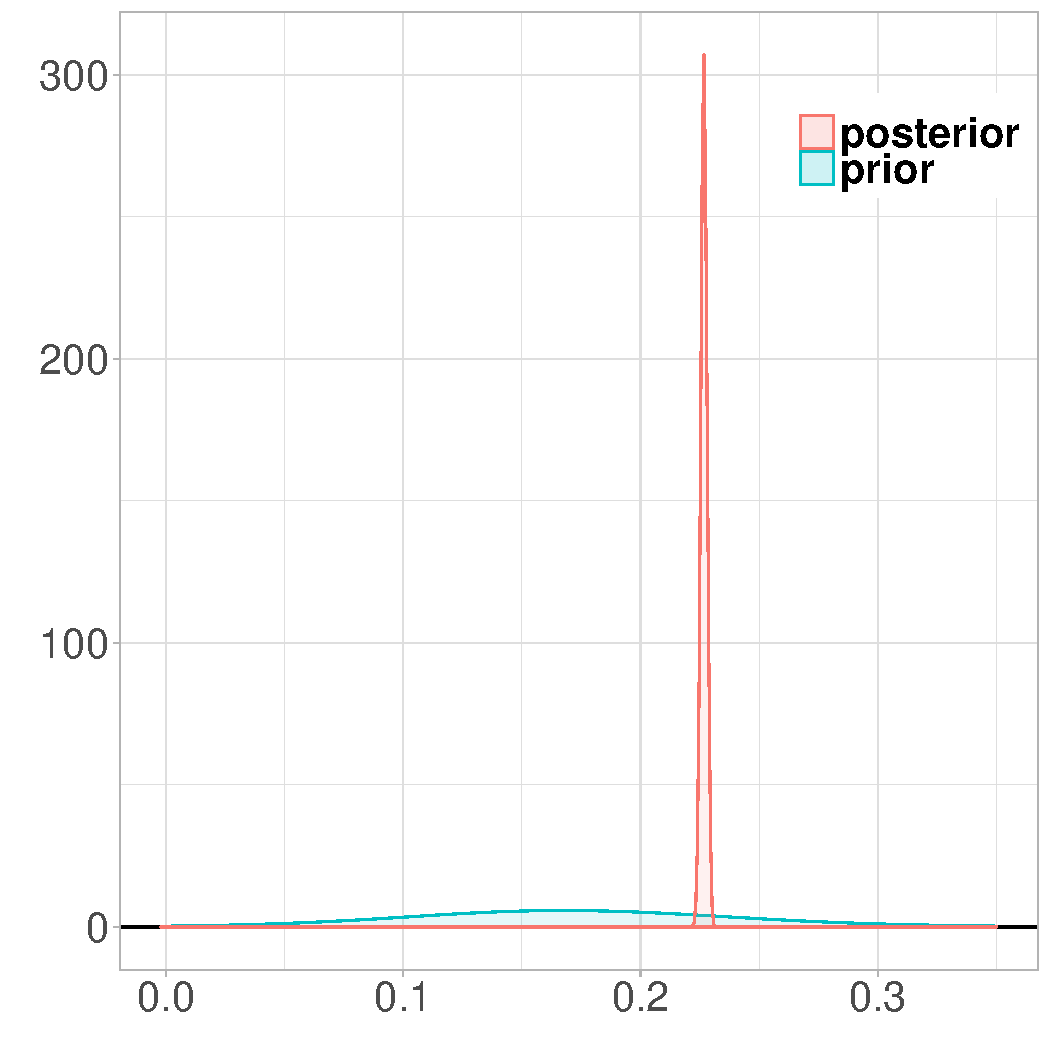
\includegraphics[width=.35\textwidth]{figR/model1/densityAr.pdf}\\
%     \end{tabular}
%    \begin{tabular}{cccccc}
%    & A \textit{priori} & $\mathcal{M}_1$ & $\mathcal{M}_2$ & $\mathcal{M}_3$
%    & $\mathcal{M}_4$\\
%	\rotatebox{90}{ \hspace{0.5em} \small Power in $W$}
%    & 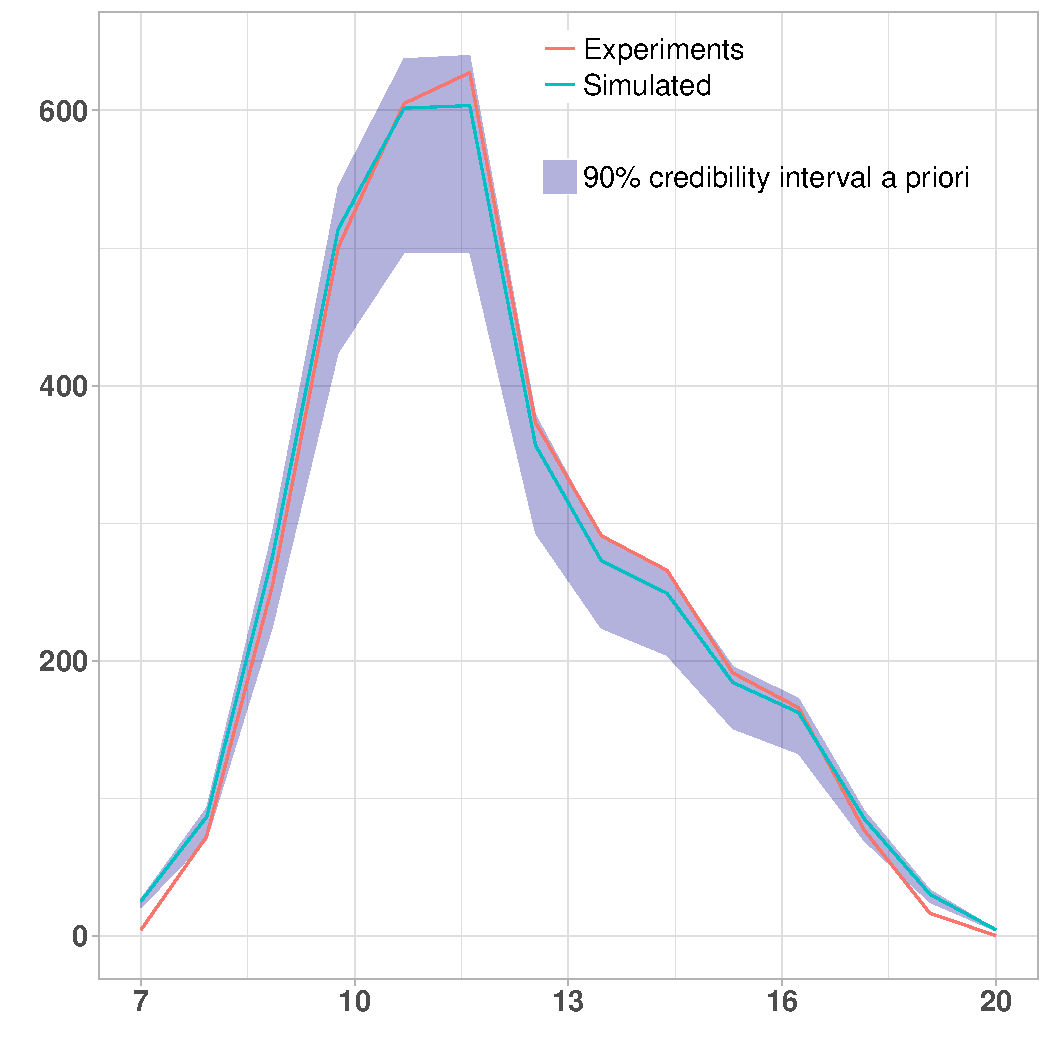
\includegraphics[width=.17\textwidth]{figR/credInterPrior.pdf}
%    & 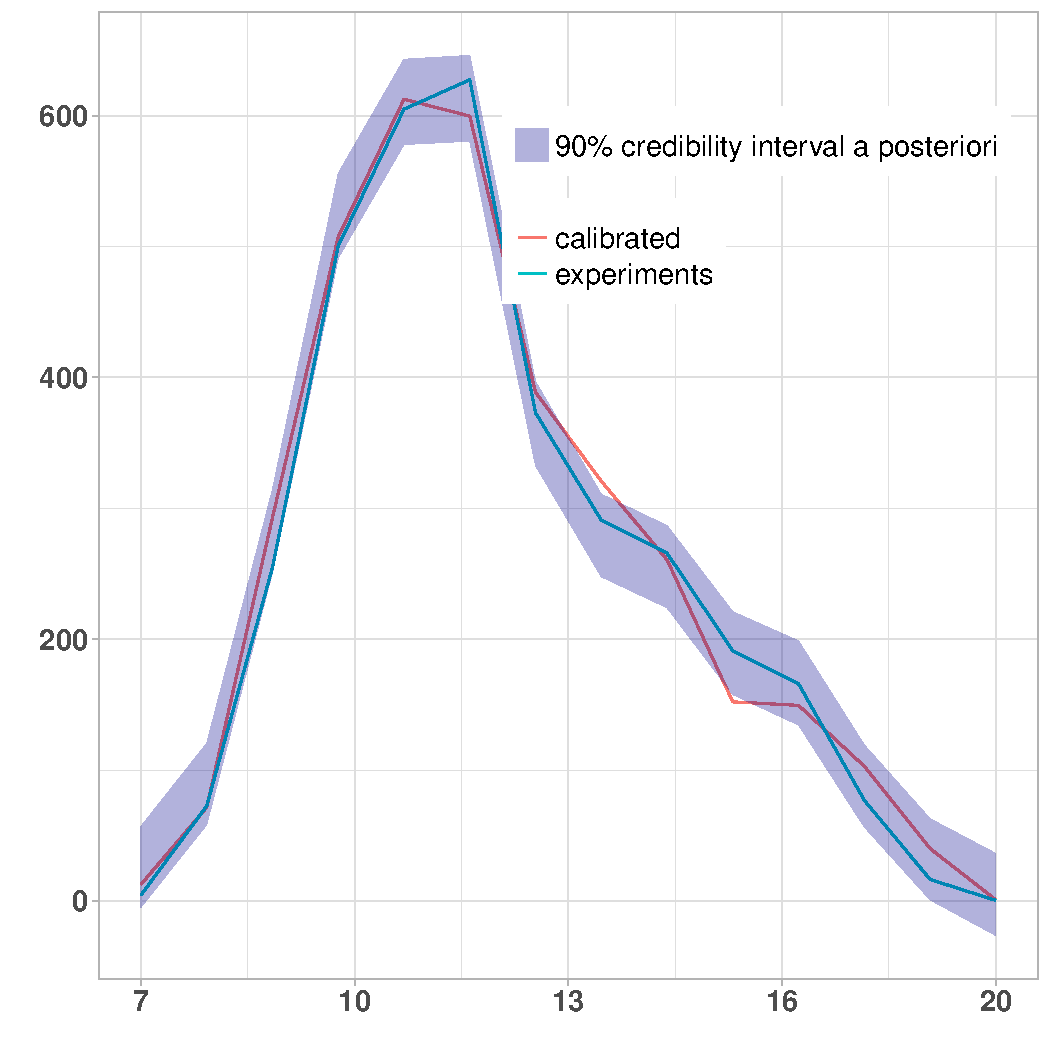
\includegraphics[width=.17\textwidth]{figR/model1Output.pdf}
%    & 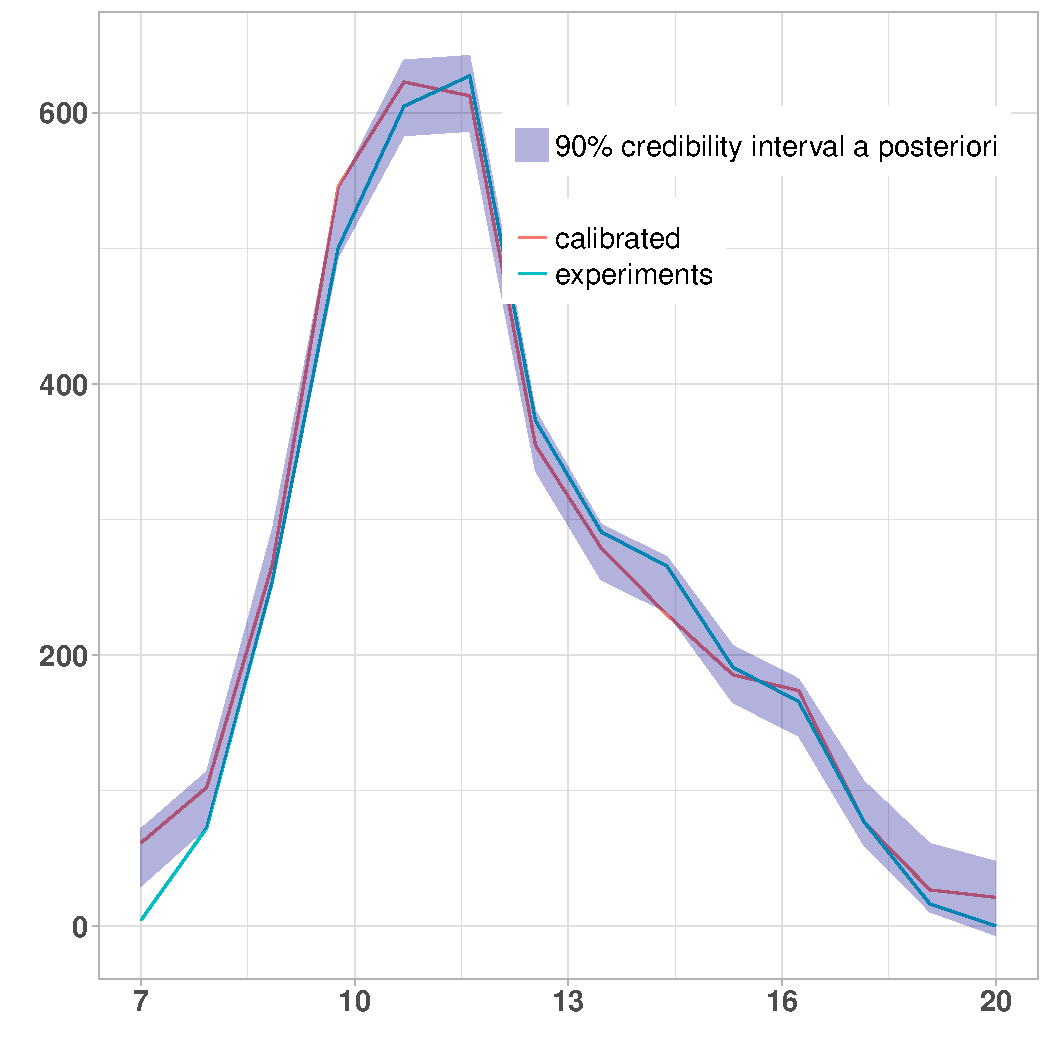
\includegraphics[width=.17\textwidth]{figR/model2Output.pdf}
%   & 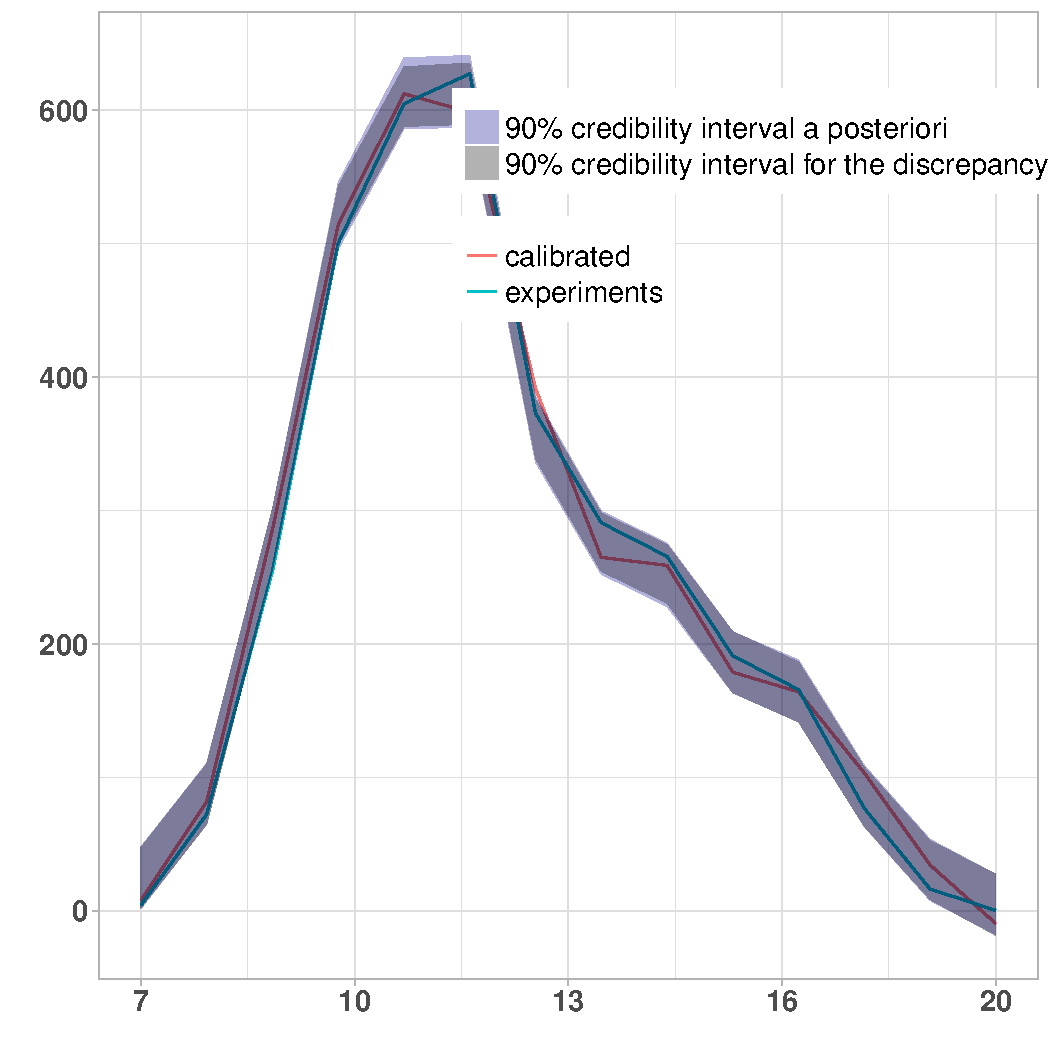
\includegraphics[width=.17\textwidth]{figR/model3Output.pdf}
%    & 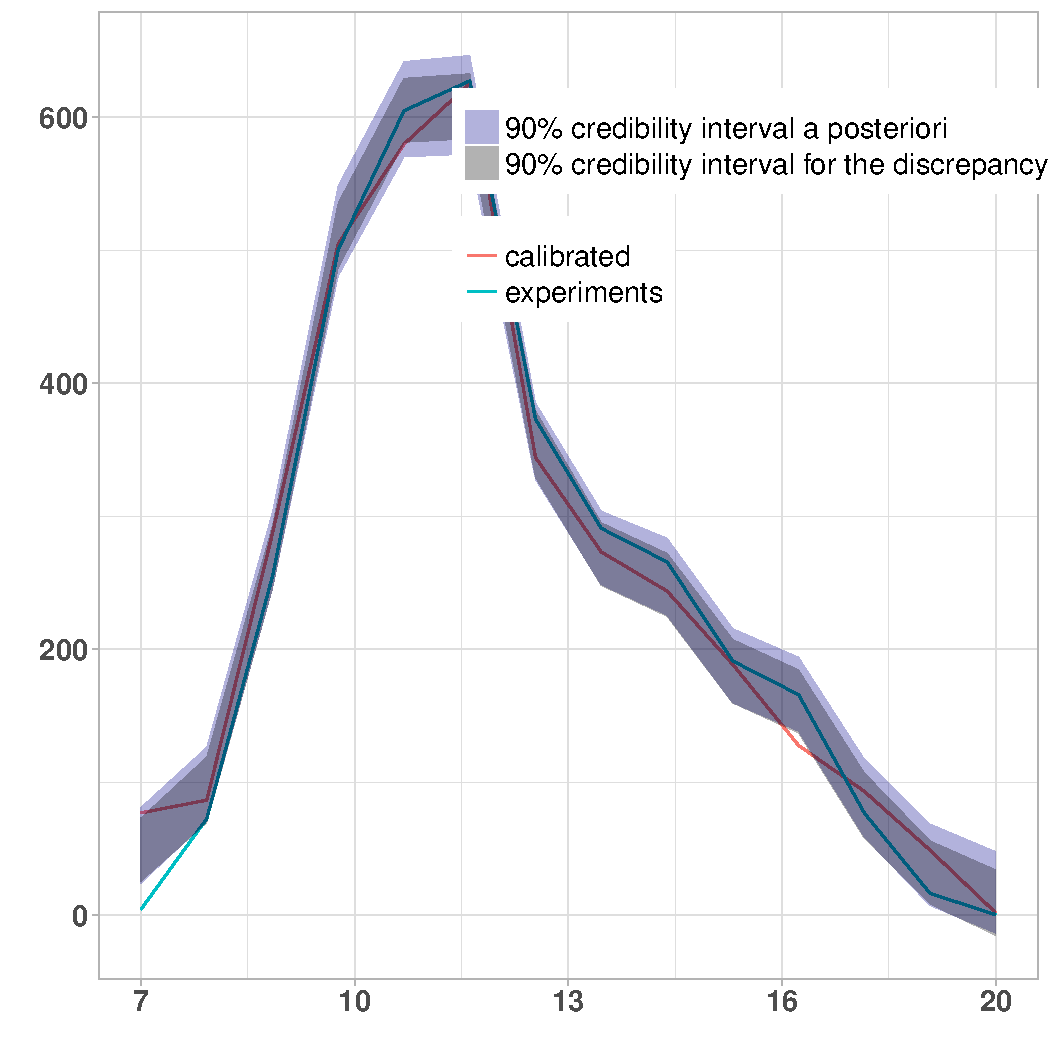
\includegraphics[width=.17\textwidth]{figR/model4Output.pdf}
%    \\
%    & \multicolumn{5}{c}{Time in hour}\\
%	&&\\
%  \end{tabular}   
%\caption{The $90\%$ credibility interval a priori is showed on the first panel against the $90\%$ credibility interval a posteriori for each models.}
%\label{fig:interestCalibration}
%\end{center}
%\end{figure}


\section{Conclusion and discussion}

This article focuses on code calibration which can be a very interesting way to deal with uncertainties in numerical experiments. The code used in the article, to allow comparisons with time consuming codes, is a quick code predicting power from small PV plant. This work can be extended to bigger computational codes in application at larger PV plants. As we are working with a physical code, it is important in this case to keep in mind the reality of the physical boundaries. This aspect had allowed us to confirm the presence of the discrepancy.\newline

In a case where input variables are correlated, additional issues of DOE appear when the surrogate is fitted. To cope with these issues we made recourse to a PCA. The design of numerical experiments could have been enhanced by using adaptive designs proposed by \citet{damblin2018}. \newline

The hypotheses made for the application case can also be discussed. For example setting $\rho$ and $m_{\delta}(.)$ to 1 and 0 is a preliminaty decision which goes along with calibration. We do not want to quantify the bias because the aim of calibration is to find the parameter value to compensate that bias. If one's goal is to check where the uncertainty goes, other hypotheses could have been made. For example, a non zero discrepancy expectation would quantify the mean of the gap between the code and the experiments. In calibration we want this gap to be taken into account in the code through adjusted $\boldsymbol{\theta}$.\newline

%The quantity of interest can also be a discussion point. If we are interested in how much the plant is going to produce over its lifetime, it is maybe more interesting to directly look into the total energy produced. In our case, the code simulates the instantaneous power. It seems unfair to establish a comparison between both quantities. We have seen that with the surrogate and the discrepancy ($\mathcal{M}_4$) the predicted energy is closer to the real value than with the code. The Gaussian processes has smoothen the phenomenons and presents better results after integration. \newline

One can wonder which models to use in a given particular case. There is no obvious answer to this question but it depends first on the numerical code. If it is time consuming, the first model to try on is $\mathcal{M}_2$ and, if it is not, one can use $\mathcal{M}_1$. One may then wonder whether it is worth adding a discrepancy term, going from $\mathcal{M}_1$ to $\mathcal{M}_3$ or from $\mathcal{M}_2$ to $\mathcal{M}_4$. In-depth work on statistical validation had been developed in \citet{damblin2016} in which the comparison between two models (with and without discrepancy) is studied in a simplified context. The Bayes factor helps to decide whether the discrepancy is relevant or not. However, this Bayes factor is burdensome to compute in a general context.




\section{Acknowledgement}
This work was supported by the research contract CIFRE n°2015/0974 between Électricité de France and AgroParisTech.

%This article has reviewed some different statistical models and has intended to clarify the use of each. The application case had shown the interest and the differences between each models. In this example, the instantaneous power represented by the computational code is not what is looked for at the end. The cumulative energy, which represents a mean of the production, is the objective. It might not be necessary to represent all instantaneous power for computing then the energy. It would be interesting to compare a surrogate and a code which compute straightforwardly the energy. \newline
%
%In some case, the interest of the add of the discrepancy remains unclear. It does not bring any improvements and it just make heavier the statistical model. Statistical validation remain a good test to select between two models. Work has be done in \cite{damblin2015} using Bayes Factor and some interesting developments have been introduced when the \textit{prior} is improper.



\newpage


\begin{appendices}
	\addtocontents{toc}{\protect\renewcommand{\protect\cftchappresnum}{Appendix }}
	\renewcommand{\chaptername}{Appendix}
	\section{Gaussian processes \label{ap:GaussianProcesses}}
	Let us consider a probability space $(\Omega,\mathcal{F},\mathbb{P})$ where $\Omega$ stands for a sample space, $\mathcal{F}$ a $\sigma$-algebra on $\Omega$ and $\mathbb{P}$ a probability on $\mathcal{F}$. A stochastic process $X$ is a family as $\{ X_t\ ;\ t\in\mathcal{T}\}$ where $\mathcal{T}\subset\mathbb{R}^d$. It is said that the aleatory process is indexed by the indexes of $\mathcal{T}$. At $t$ fixed, the application $X_t \ : \ \Omega \rightarrow \mathbb{R}$ is an random variable. However at $\omega \in \Omega$ fixed, the application $ t \rightarrow X_t(\omega)$ is a trajectory of the stochastic process.\newline


For $t_1 \in \mathcal{T},\dots, t_n\in\mathcal{T}$, the probability distribution of the random vector $(X_{t_1},\dots,X_{t_n})$ is called finite-dimensional distributions of the stochastic process $\{X_t\}_{t\in\mathcal{T}}$. Hence, the probability distribution of an aleatory process is determined by its finite-dimensional distributions. Kolmogorov's theorem guaranties the existence of such a stochastic process if a suitably collection of coherent finite-dimensional distributions is provided.\newline

An random vector $\boldsymbol{Z}$ such as $\boldsymbol{Z}=(Z_1,\dots,Z_n)$ is Gaussian if $\forall \lambda_1,\dots,\lambda_n \in \mathbb{R}$ the random variable $\sum_{i=1}^n\lambda_iZ_i$ is Gaussian. The distribution of $Z$ is straightforwardly determined by its two first moments \hc the mean $\boldsymbol{\mu}=(\mathbb{E}[Z_1],\dots,\mathbb{E}[Z_n])$ and the variance covariance matrix $\Sigma = cov(Z_i,Z_j)_{1\leq i,\ j\leq n}$. When $\Sigma$ is positive definite, $Z$ has a probability density defined by equation (\ref{eq:densityGaussian}). \newline

\begin{equation}
f(\bm{z})=\frac{|\Sigma|^{-1/2}}{(2\pi)^{n/2}}\exp \Big\{-\frac{1}{2}(\boldsymbol{z}-\boldsymbol{\mu})^T\Sigma^{-1}(\boldsymbol{z}-\boldsymbol{\mu}) \Big\}
\label{eq:densityGaussian}
\end{equation}

Let us consider two Gaussian vectors called $\bm{U_1}$ and $\boldsymbol{U_2}$ such as\hc \newline

\begin{equation*}
\begin{pmatrix}
\bm{U_1}\\
\bm{U_2}
\end{pmatrix} \sim \mathcal{N} \Big( \begin{pmatrix}
\bm{\mu_1}\\
\bm{\mu_2}
\end{pmatrix}, \begin{pmatrix}
\Sigma_{1,1} & \Sigma_{1,2}\\
\Sigma_{2,1} & \Sigma_{2,2}
\end{pmatrix} \Big)
\end{equation*}

The conditional distribution $\bm{U_2}|\bm{U_1}$ is also Gaussian (Equation (\ref{eq:conditionalGaussian})). This property is especially useful when a surrogate model is created from a code. \newline

\begin{equation}
\bm{U_2}|\bm{U_1} \sim \mathcal{N}(\bm{\mu_2}+\Sigma_{2,1}\Sigma_{1,1}^{-1}(\bm{U_1}-\bm{\mu_1}), \Sigma_{2,2}-\Sigma_{2,1}\Sigma_{1,1}^{-1}\Sigma_{1,2})
\label{eq:conditionalGaussian}
\end{equation}


A stochastic process $\{X_t\}_{t\in\mathcal{T}}$ is a Gaussian process if each of its finite-dimensional distributions is Gaussian. Let us introduce the mean function such as $m : t\in\mathcal{T} \rightarrow m(t)=\mathbb{E}[X_t]$ and the correlation function such as $ K : (t,t')\in\mathcal{T}\times \mathcal{T}\rightarrow K(t,t')=corr(X_t,X_{t'})$. A Gaussian process with a scale parameter noted $\sigma^2$ will be defined as the equation (\ref{eq:GaussianDef}).

\begin{equation}
X(.) \sim \mathcal{PG}(m(.),\sigma^2K(.,.))
\label{eq:GaussianDef}
\end{equation}

Gaussian processes are used in this article in two cases. In the fist one, $f$ is a code function long to run and the Gaussian process emulates its behavior. The Gaussian process is called the surrogate of the code. The second case is when we want to estimate the error made by the code (called code error or discrepancy in this article). For the former, we want to create a surrogate $\tilde{f}$ of a deterministic function $f$. In a Bayesian framework, the Gaussian process is a "functional" \textit{a priori} on $f$ \citep{currin1991}.\newline

Let us note\hc
\begin{equation}
f(.) \sim \mathcal{PG}(h(.)^T\boldsymbol{\beta}_f,\sigma_f^2K_{\boldsymbol{\psi}_f}(.,.))
\end{equation}
where $\boldsymbol{\beta}_f$, $\sigma_f^2$, $\boldsymbol{\psi}_f$ are the parameters specifying the mean and the variance-covariance structure of the process and $h(t)=(h_1(t),\dots,h_n(t))$ is a vector of regressors. For $(t,t')\in \mathcal{T}\times\mathcal{T}$\hc
\begin{equation}
cov(f(t),f(t'))=\sigma_f^2K_{\boldsymbol{\psi}_f}(t,t')
\end{equation}

Let us consider the code have been tested on $N$ points \textit{i.e.} on $N$ different vectors $\bm{t}$. The design of experiments (DOE) is noted $D=(t_1,\dots,t_N)^T$ and the outputs of $D$ by $f$ will be defined as $y=(f(t_1),\dots,f(t_N))^T$. The correlation matrix  induced by $y$ can be defined by the correlation function $K_{\boldsymbol{\psi}_f}(.,.)$ and can be written as $\Sigma_{\boldsymbol{\psi}_f}(D)=\Sigma_{\boldsymbol{\psi}_f}(D,D)$ such as $\forall (i,j) \in [1,\dots,n] \  \Sigma_{\boldsymbol{\psi}_f}(D)(i,j)=K_{\boldsymbol{\psi}_f}(t_i,t_j)$.

\begin{equation}
\begin{pmatrix}
f(t)\\
f(D)
\end{pmatrix} \sim \mathcal{N}\Big( \begin{pmatrix}
h(t)^T\boldsymbol{\beta}_f\\
h(D)^T\boldsymbol{\beta}_f
\end{pmatrix}, \sigma_f^2\begin{pmatrix}
\Sigma_{\boldsymbol{\psi}_f}(t) &  \Sigma_{\boldsymbol{\psi}_f}(t,D) \\
\Sigma_{\boldsymbol{\psi}_f}(t,D)^T & \Sigma_{\boldsymbol{\psi}_f}(D)
\end{pmatrix}\Big)
\label{eq:Conditionnal}
\end{equation}

From Equation (\ref{eq:conditionalGaussian}), it comes straightforwardly that $f(t)|f(D)\sim\mathcal{PG}(\mu_p(t),\Sigma_p(t))$. This conditional is called \textit{posterior} distribution with \hc
\begin{equation*}
\mu_p(t)=h(t)^T\boldsymbol{\beta}_f+\Sigma_{\boldsymbol{\psi}_f}(t,D)\Sigma_{\boldsymbol{\psi}_f}(D)^{-1}(f(D)-h(D)^T\boldsymbol{\beta}_f)
\end{equation*} 
\begin{equation*}
\Sigma_p(t,t')=\sigma_f^2\Big(\Sigma_{\boldsymbol{\psi}_f}(t,t')-\Sigma_{\boldsymbol{\psi}_f}(t,D)^T\Sigma_{\boldsymbol{\psi}_f}(D)^{-1}\Sigma_{\boldsymbol{\psi}_f}(t',D)\Big)
\end{equation*}

The mean obtained \textit{a posteriori} is called the Best Linear Unbiased Predictor (BLUP) which the linear predictor without bias $\tilde{f}$ of $f$ which minimize the Mean Square Error (MSE) \hc
\begin{equation}
MSE(\tilde{f})=\mathbb{E}[(f-\tilde{f})^2]
\end{equation}

In this appendix, we will not discuss the choice of $K_{\boldsymbol{\psi}_f}$, the parameter estimation, nor the validation of the Gaussian process.
\newpage

\end{appendices}





\bibliography{biblio}




\end{document}
